\documentclass[twoside]{book}

% Packages required by doxygen
\usepackage{calc}
\usepackage{doxygen}
\usepackage{graphicx}
\usepackage[utf8]{inputenc}
\usepackage{makeidx}
\usepackage{multicol}
\usepackage{multirow}
\usepackage{textcomp}
\usepackage[table]{xcolor}

% Font selection
\usepackage[T1]{fontenc}
\usepackage{mathptmx}
\usepackage[scaled=.90]{helvet}
\usepackage{courier}
\usepackage{amssymb}
\usepackage{sectsty}
\renewcommand{\familydefault}{\sfdefault}
\allsectionsfont{%
  \fontseries{bc}\selectfont%
  \color{darkgray}%
}
\renewcommand{\DoxyLabelFont}{%
  \fontseries{bc}\selectfont%
  \color{darkgray}%
}

% Page & text layout
\usepackage{geometry}
\geometry{%
  letterpaper,%
  top=2.5cm,%
  bottom=2.5cm,%
  left=2.5cm,%
  right=2.5cm%
}
\tolerance=750
\hfuzz=15pt
\hbadness=750
\setlength{\emergencystretch}{15pt}
\setlength{\parindent}{0cm}
\setlength{\parskip}{0.2cm}
\makeatletter
\renewcommand{\paragraph}{%
  \@startsection{paragraph}{4}{0ex}{-1.0ex}{1.0ex}{%
    \normalfont\normalsize\bfseries\SS@parafont%
  }%
}
\renewcommand{\subparagraph}{%
  \@startsection{subparagraph}{5}{0ex}{-1.0ex}{1.0ex}{%
    \normalfont\normalsize\bfseries\SS@subparafont%
  }%
}
\makeatother

% Headers & footers
\usepackage{fancyhdr}
\pagestyle{fancyplain}
\fancyhead[LE]{\fancyplain{}{\bfseries\thepage}}
\fancyhead[CE]{\fancyplain{}{}}
\fancyhead[RE]{\fancyplain{}{\bfseries\leftmark}}
\fancyhead[LO]{\fancyplain{}{\bfseries\rightmark}}
\fancyhead[CO]{\fancyplain{}{}}
\fancyhead[RO]{\fancyplain{}{\bfseries\thepage}}
\fancyfoot[LE]{\fancyplain{}{}}
\fancyfoot[CE]{\fancyplain{}{}}
\fancyfoot[RE]{\fancyplain{}{\bfseries\scriptsize Generated on Sat Apr 11 2015 12\-:43\-:11 for Poly\-D\-A\-Q by Doxygen }}
\fancyfoot[LO]{\fancyplain{}{\bfseries\scriptsize Generated on Sat Apr 11 2015 12\-:43\-:11 for Poly\-D\-A\-Q by Doxygen }}
\fancyfoot[CO]{\fancyplain{}{}}
\fancyfoot[RO]{\fancyplain{}{}}
\renewcommand{\footrulewidth}{0.4pt}
\renewcommand{\chaptermark}[1]{%
  \markboth{#1}{}%
}
\renewcommand{\sectionmark}[1]{%
  \markright{\thesection\ #1}%
}

% Indices & bibliography
\usepackage{natbib}
\usepackage[titles]{tocloft}
\setcounter{tocdepth}{3}
\setcounter{secnumdepth}{5}
\makeindex

% Hyperlinks (required, but should be loaded last)
\usepackage{ifpdf}
\ifpdf
  \usepackage[pdftex,pagebackref=true]{hyperref}
\else
  \usepackage[ps2pdf,pagebackref=true]{hyperref}
\fi
\hypersetup{%
  colorlinks=true,%
  linkcolor=blue,%
  citecolor=blue,%
  unicode%
}

% Custom commands
\newcommand{\clearemptydoublepage}{%
  \newpage{\pagestyle{empty}\cleardoublepage}%
}


%===== C O N T E N T S =====

\begin{document}

% Titlepage & ToC
\hypersetup{pageanchor=false}
\pagenumbering{roman}
\begin{titlepage}
\vspace*{7cm}
\begin{center}%
{\Large Poly\-D\-A\-Q \\[1ex]\large 2.\-1 }\\
\vspace*{1cm}
{\large Generated by Doxygen 1.8.6}\\
\vspace*{0.5cm}
{\small Sat Apr 11 2015 12:43:11}\\
\end{center}
\end{titlepage}
\clearemptydoublepage
\tableofcontents
\clearemptydoublepage
\pagenumbering{arabic}
\hypersetup{pageanchor=true}

%--- Begin generated contents ---
\chapter{Main Page}
\label{index}\hypertarget{index}{}\hypertarget{index_Introduction}{}\section{Introduction}\label{index_Introduction}
Poly\-D\-A\-Q is a customizable, embeddable data acquisition device for educational use. It was originally designed for use in the Cal Poly Mechanical Engineering Thermal Laboratory, but it has been improved with the intention that it will be usable for many different applications. It can function as a data acquisition card for a small computer or a standalone datalogger. All hardware and software is open source.\hypertarget{index_Links}{}\section{Links}\label{index_Links}
\begin{DoxyItemize}
\item \hyperlink{pd_setup}{Power and Data} For Poly\-D\-A\-Q setup of power and data connections \item \hyperlink{pd_sensors}{Connecting Sensors} For information about how to connect various types of sensors \item \hyperlink{pd_channels}{Channel Commands} For tables which show the commands used to access the data channels on each Poly\-D\-A\-Q 2 board version \item \hyperlink{pd_py_gui}{The Python G\-U\-I} For a user guide to operating the Poly\-D\-A\-Q G\-U\-I, which runs on Windows$^{\mbox{T\-M}}$ , Mac$^{\mbox{T\-M}}$ , and Linux$^{\mbox{T\-M}}$  computers.\end{DoxyItemize}
\hypertarget{index_Sensors}{}\section{Sensors}\label{index_Sensors}
Poly\-D\-A\-Q's hardware features include thermocouple, voltage, strain, and acceleration inputs. Although traces are present on the board to accommodate all of these features, some features may be left off an individual board to save money and electric power. In addition, several versions of Poly\-D\-A\-Q have the same processor and run the same software but are equipped with different sets of sensors\-: \begin{DoxyItemize}
\item Four thermocouple inputs, using A\-D8494 or A\-D8495 thermocouple signal conditioners for linear amplification and cold junction compensation. \item Four voltage inputs. Some voltage inputs use a moderately high input resistance voltage divider and an op-\/amp voltage follower with level shifter to allow an input range of -\/10 to +10 volts. This scheme is similar to that used in other low-\/cost D\-A\-Q devices such as the U\-S\-B-\/600\-X series from National Instruments(tm). Other voltage inputs can be set up without voltage dividers to give 0-\/3.\-3\-V full-\/scale measurements. The A/\-D converters use a precision 3.\-3\-V reference for accuracy. \item Up to four strain gauge bridge amplifiers whose I\-N\-A122 instrumentation amplifiers allow resolution down to the microstrain in typical Wheatstone bridge applications.\end{DoxyItemize}
\hypertarget{index_Components}{}\section{Components}\label{index_Components}
Basic components common to all Poly\-D\-A\-Q 2's include the following\-: \begin{DoxyItemize}
\item An S\-T\-M32\-F4 microcontroller which controls the data acquisition process and communicates with a P\-C (if used). \item A U\-S\-B-\/serial interface which can supply power to the board through the U\-S\-B cable as well as communicate between the Poly\-D\-A\-Q and the computer. Power can also be supplied as 5 -\/ 12 volts D\-C through a standard barrel jack. \item A Bluetooth serial modem for wireless communication with laptops, tablets, or phones (if installed). \item A micro-\/\-S\-D card socket. S\-D cards of up to around 32\-G\-B capacity can be used, and data is stored in files using the old D\-O\-S low-\/level format. C\-S\-V text files are the standard file format, but other file formats can be utilized with small changes to the firmware. Using S\-D\-I\-O card access rather than the slower S\-P\-I protocol, data has been saved at up to 36\-K\-B/s in tests so far, and we expect speed improvements as the software is refined. \item Programmability (to flash updated firmware) through a 6-\/pin S\-T\-Link2 connector.\end{DoxyItemize}
\hypertarget{index_Firmware}{}\section{Firmware}\label{index_Firmware}
The Poly\-D\-A\-Q firmware is based on the S\-T\-M32 Standard Peripheral Library and Free\-R\-T\-O\-S. This software was chosen for its compatibility with software used in Cal Poly M\-E mechatronics courses, which was in turn selected as the preferred R\-T\-O\-S environment for educational use. Free\-R\-T\-O\-S isn't known as an especially high performance R\-T\-O\-S, but its internal structure is more easily understood than those of many competing products -\/ multithreading and device access are not as hidden from the application programmer as in many other R\-T\-O\-Ses, so students can learn more about many important fundamentals. Performance is not that much of an issue, especially when we have an S\-T\-M32\-F4 processor which runs at 168 M\-Hz and has hardware floating point support.

G\-U\-I applications are being written for use on major P\-C operating systems (Linux, Mac$^{\mbox{T\-M}}$ , Windows$^{\mbox{T\-M}}$ ) and if we have good luck in porting, Android$^{\mbox{T\-M}}$ . The applications are written in Python and use the Qt G\-U\-I libraries, Num\-Py, and Py\-Qwt.\hypertarget{index_Version}{}\section{Version}\label{index_Version}
This page documents Poly\-D\-A\-Q Version 2.\-1. As of this writing (March 2015), Poly\-D\-A\-Q 2 is a work in progress. Prototypes have been made and are undergoing testing, and a production run of a dozen or so boards is being produced. 
\chapter{Channel Commands}
\label{pd_channels}
\hypertarget{pd_channels}{}
This page contains tables showing which channels are accessed by which channel commands on different versions of the Poly\-D\-A\-Q 2 board. These channel commands can be used in the data logger configuration file and when communicating with a Poly\-D\-A\-Q through the dumb terminal.

All commands are {\bfseries case} {\bfseries sensitive}. For example, typing {\bfseries D} will cause the Poly\-D\-A\-Q to perform an A/\-D conversion on the channel specified by the hexadecimal number D (decimal 13), but typing {\bfseries d} will cause the Poly\-D\-A\-Q to show the results of a memory dump (a programming diagnostic tool).

When a command is not understood by the Poly\-D\-A\-Q, it shows the command which has confused it and asks, \char`\"{}\-What's That Function?\char`\"{}\hypertarget{pd_channels_pd_044}{}\section{Poly\-D\-A\-Q 0-\/4-\/4}\label{pd_channels_pd_044}
This version of the Poly\-D\-A\-Q 2 board is designed for use in the M\-E 410 course, which makes heavy use of strain gauges. It has four strain gauge bridge amplifiers and four voltage inputs. Two of the voltage inputs accept -\/10 to +10\-V inputs and the other two accept 0 to 3.\-3\-V inputs with finer resolution. If present, an onboard M\-M\-A8452\-Q accelerometer provides 3 axes of acceleration data. An external M\-M\-A8452\-Q accelerometer can be connected to the board's I2\-C bus; if present, the external accelerometer is accessed as shown in the table.

The given calibration numbers (slope and offset) are approximate and for convenience only. The user should check all calibrations carefully using a high-\/accuracy voltmeter. In many cases, entering a slope of 1.\-0 and offset of 0.\-0 to cause raw A/\-D output numbers to be recorded is the best option.

\begin{TabularC}{5}
\hline
\rowcolor{lightgray}\PBS\centering {\bf Channel }&\PBS\centering {\bf Command }&\PBS\centering {\bf Slope }&\PBS\centering {\bf Offset }&{\bf Description  }\\\cline{1-5}
\PBS\centering {\ttfamily S1} &\PBS\centering {\ttfamily E} &\PBS\centering 0.\-00806 (1) &\PBS\centering (2) &Strain gauge bridge 1 \\\cline{1-5}
\PBS\centering {\ttfamily S2} &\PBS\centering {\ttfamily F} &\PBS\centering 0.\-00806 (1) &\PBS\centering (2) &Strain gauge bridge 2 \\\cline{1-5}
\PBS\centering {\ttfamily S3} &\PBS\centering {\ttfamily 9} &\PBS\centering 0.\-00806 (1) &\PBS\centering (2) &Strain gauge bridge 3 \\\cline{1-5}
\PBS\centering {\ttfamily S4} &\PBS\centering {\ttfamily 8} &\PBS\centering 0.\-00806 (1) &\PBS\centering (2) &Strain gauge bridge 4 \\\cline{1-5}
\PBS\centering &\PBS\centering &\PBS\centering &\PBS\centering &\\\cline{1-5}
\PBS\centering {\ttfamily V1} &\PBS\centering {\ttfamily A} &\PBS\centering 0.\-00513 &\PBS\centering -\/8.\-8537 &Voltage channel 1 (-\/10 to +10\-V) \\\cline{1-5}
\PBS\centering {\ttfamily V2} &\PBS\centering {\ttfamily B} &\PBS\centering 0.\-00513 &\PBS\centering -\/8.\-8537 &Voltage channel 2 (-\/10 to +10\-V) \\\cline{1-5}
\PBS\centering {\ttfamily V3} &\PBS\centering {\ttfamily C} &\PBS\centering 0.\-000806 &\PBS\centering 0.\-0 &Voltage channel 3 (0 to +3.3\-V) \\\cline{1-5}
\PBS\centering {\ttfamily V4} &\PBS\centering {\ttfamily D} &\PBS\centering 0.\-000806 &\PBS\centering 0.\-0 &Voltage channel 4 (0 to +3.3\-V) \\\cline{1-5}
\PBS\centering &\PBS\centering &\PBS\centering &\PBS\centering &\\\cline{1-5}
\PBS\centering {\ttfamily X} &\PBS\centering {\ttfamily X} &\PBS\centering 0.\-000061 (3) &\PBS\centering 0.\-0 &Onboard accelerometer X axis \\\cline{1-5}
\PBS\centering {\ttfamily Y} &\PBS\centering {\ttfamily Y} &\PBS\centering 0.\-000061 (3) &\PBS\centering 0.\-0 &Onboard accelerometer Y axis \\\cline{1-5}
\PBS\centering {\ttfamily Z} &\PBS\centering {\ttfamily Z} &\PBS\centering 0.\-000061 (3) &\PBS\centering 0.\-0 &Onboard accelerometer Z axis \\\cline{1-5}
\PBS\centering &\PBS\centering &\PBS\centering &\PBS\centering &\\\cline{1-5}
\PBS\centering {\ttfamily x} &\PBS\centering {\ttfamily x} &\PBS\centering 0.\-000061 (3) &\PBS\centering 0.\-0 &External accelerometer X axis \\\cline{1-5}
\PBS\centering {\ttfamily y} &\PBS\centering {\ttfamily y} &\PBS\centering 0.\-000061 (3) &\PBS\centering 0.\-0 &External accelerometer Y axis \\\cline{1-5}
\PBS\centering {\ttfamily z} &\PBS\centering {\ttfamily z} &\PBS\centering 0.\-000061 (3) &\PBS\centering 0.\-0 &External accelerometer Z axis \\\cline{1-5}
\end{TabularC}
Notes\-: \par
 (1) The given slope converts A/\-D output to bridge differential voltage in m\-V. \par
 (2) Bridge amplifier offset varies depending on bridge balance. \par
 (3) When the accelerometer is configured for +/-\/2g range, as is its default. 
\chapter{The Python G\-U\-I}
\label{pd_py_gui}
\hypertarget{pd_py_gui}{}
This page describes how to use the Poly\-D\-A\-Q G\-U\-I application. This application is written in the Python language, is open source to all who dare try to read and deal with it, and runs on many platforms -- at least Windows$^{\mbox{T\-M}}$ , Mac$^{\mbox{T\-M}}$ , and Linux$^{\mbox{T\-M}}$ .

 
\begin{DoxyImageNoCaption}
  \mbox{\includegraphics{gui_screenshot_1.png}}
\end{DoxyImageNoCaption}
\hypertarget{pd_py_gui_gui_steps}{}\section{Running the G\-U\-I}\label{pd_py_gui_gui_steps}
To set up and start data collection, follow the following steps\-:
\begin{DoxyEnumerate}
\item {\bfseries Initilize the communication port\-:} Under Initial Settings, click {\ttfamily C\-H\-O\-O\-S\-E} {\ttfamily P\-O\-R\-T} and select the port corresponding to your hardware (Linux\-: usually {\ttfamily /dev/tty\-U\-S\-B0}; Windows$^{\mbox{T\-M}}$ \-: usually {\ttfamily C\-O\-M3} or {\ttfamily C\-O\-M4}, always {\ttfamily C\-O\-M} {\itshape something}.) The status window will indicate that the hardware has been connected and the rest of the interface will be activated. Note\-: If the interface is not activated, check the status window\-: the hardware may not have been connected, or you may not have permission to access the serial port.
\item {\bfseries Change data filename} (optional)\-: The default filename is the date and time you opened the program. This name is unique and will help you identify your file later; however, you may change the file name if you wish.
\item {\bfseries Select channels} and edit channel names\-: Click the boxes coresponding to the channels you wish to record. You may also customize the names of any channel in order to make data labels more meaningful. These names are what will appear in your data file.
\item {\bfseries Balance strain gauge bridges\-:} Strain gauge Wheatstone bridges require balancing prior to start. To run an auto-\/balance on the strain bridges, go to the main menu bar and select {\ttfamily Hardware} -\/$>$ {\ttfamily Auto-\/balance Strain Gauges...}
\item {\bfseries Choose sample rate} and options\-: Select the desired sample rate using the combo box. The sample rate varies slightly due to how the hardware works, but the data file records actual time of measurements, so accurate signal-\/time plots can still be made.

Some sample rates are only achievable if you select fewer channels; this is noted in the combo box.

You can set the D\-A\-Q to record until a specified time, then automatically stop. By default, data is taken until you manually stop it.
\item {\bfseries Start and Stop\-:} These two buttons do exactly what one would expect. Note that after the D\-A\-Q is started, the control panel is inactivated; you cannot change data acquisition parameters while collecting data.
\end{DoxyEnumerate}\hypertarget{pd_py_gui_gui_nav}{}\section{Live Data Navigation}\label{pd_py_gui_gui_nav}
You can explore the data while it is being collected. The latest numerical value for each channel is displayed in the plot legend. The live plot can be navigated in the following ways\-:
\begin{DoxyItemize}
\item {\bfseries y-\/axis controls\-:} Right-\/clicking on the y axis opens a menu where you can
\begin{DoxyItemize}
\item Zoom all y\-: expands the y axis to include the entire range of y values collected {\itshape so} {\itshape far} 
\item Manually set axis limits
\item Turn Auto\-Scale on/off\-: automatically adjust the y-\/axis limits as data is being collected
\end{DoxyItemize}
\item {\bfseries time axis controls\-:} Right-\/clicking the time axis opens a menu where you can
\begin{DoxyItemize}
\item Zoom all time\-: zooms out to display the entire time data has been collected
\item Manually set axis limits
\item Synchronize time axes\-: When more than one plot is displayed, this function updates all plots to the same time range when you pan or zoom in another plot
\end{DoxyItemize}
\item {\bfseries Line display controls\-:} Right-\/clicking on any signal in the plot legend to the right of the plot allows you to
\begin{DoxyItemize}
\item Turn the curve off, to make viewing other channels' data easier. Making the line invisible from the plot does not affect the data being recorded to the data file
\item Change the line properties like color and line thickness
\end{DoxyItemize}
\item {\bfseries Mouse controls\-:} allow panning and zooming
\begin{DoxyItemize}
\item Zoom Window\-: left click-\/and-\/drag draws a rectangle on the plot, then the view zooms in to that rectangle
\item Scroll-\/wheel Zoom\-: using the scroll wheel on your mouse also zooms in or out
\item Pan\-: clicking and dragging on the scroll wheel (middle mouse button) allows you to pan within the plot
\item Undo zoom\-: right-\/clicking anywhere within the plot returns the plot to the previous zoom state 
\end{DoxyItemize}
\end{DoxyItemize}
\chapter{Power and Data}
\label{pd_setup}
\hypertarget{pd_setup}{}
This page describes how to connect a Poly\-D\-A\-Q to power and communication circuits.\hypertarget{pd_setup_pds_power}{}\section{Power}\label{pd_setup_pds_power}
The Poly\-D\-A\-Q 2 has two power connections; either may be used\-:
\begin{DoxyItemize}
\item A mini-\/\-U\-S\-B connector supplies power and enables communication to a P\-C. If communication is not needed, a U\-S\-B charger can be used to power the board for data logging. Note that this is {\itshape not} a micro-\/\-U\-S\-B as is used by many cell phones and e-\/readers but a slightly larger \char`\"{}\-Mini B\char`\"{} plug.
\item A standard \char`\"{}barrel jack\char`\"{} connector allows the Poly\-D\-A\-Q 2 to be supplied from a battery or a \char`\"{}wall wart\char`\"{} type plug-\/in power supply. Such an external power supply must be rated at 5 volts to 12 volts with at least 250m\-A of current capacity. Batteries should supply a voltage between 5 volts and 9 volts. A direct connection to an automotive electrical circuit should {\bfseries not} be used because most automotive circuits produce voltage spikes that can destroy a Poly\-D\-A\-Q. Use a separate battery or plug-\/in U\-S\-B charger for automotive applications.
\end{DoxyItemize}\hypertarget{pd_setup_pds_serial}{}\section{Serial Communications}\label{pd_setup_pds_serial}
The mini-\/\-U\-S\-B connector on the Poly\-D\-A\-Q 2 can be used for serial communication between the Poly\-D\-A\-Q and a desktop or laptop computer. When a Poly\-D\-A\-Q is connected via U\-S\-B to a properly configured P\-C, a U\-S\-B serial port connection is automatically made.
\begin{DoxyItemize}
\item {\bfseries Linux} computers are configured to communicate with a Poly\-D\-A\-Q out of the box -- no additional drivers are needed. The U\-S\-B serial port will be named {\ttfamily /dev/tty\-U\-S\-B0} if no other similar U\-S\-B serial device is connected. If other U\-S\-B serial devices are connected, the Poly\-D\-A\-Q can be named {\ttfamily /dev/tty\-U\-S\-B1}, or {\ttfamily /dev/tty\-U\-S\-B2}, {\itshape etc}.
\item {\bfseries Windows(tm)} computers often need to have drivers installed for the U\-S\-B serial chip on the Poly\-D\-A\-Q. Windows(tm) often recognizes the U\-S\-B serial chip when it's plugged into the U\-S\-B port and automatically installs the correct drivers. When it does not, drivers for the F\-T232\-R\-L chip are available at {\ttfamily \href{http://www.ftdichip.com}{\tt http\-://www.\-ftdichip.\-com}}. When the drivers are working, the Poly\-D\-A\-Q's serial port will then be named {\ttfamily C\-O\-M3} or {\ttfamily C\-O\-M4} or {\ttfamily C\-O\-M5} or something similar, depending on how many virtual serial port devices have been plugged into the computer before.
\item {\bfseries Mac(tm)} computers do something really cool and shiny but we're not sure what because we can't afford one. This section will be updated after we've had a chance to borrow a Mac(tm) from one of the Cool Kids and try it.
\end{DoxyItemize}

The U\-S\-B serial port can be accessed from a desktop or laptop computer using the Poly\-D\-A\-Q 2 G\-U\-I (see the \hyperlink{pd_py_gui}{Poly\-D\-A\-Q G\-U\-I} page for details) or through a dumb terminal emulator program. A \char`\"{}dumb terminal\char`\"{} is a program which allows the user to type characters which are immediately sent to the Poly\-D\-A\-Q and to see characters which the Poly\-D\-A\-Q has sent back; the terminal is called \char`\"{}dumb\char`\"{} because it does little or no processing of the characters -- it just sends and receives them unthinkingly. There are many dumb terminal programs available for free\-:
\begin{DoxyItemize}
\item {\bfseries Linux} computers can use Pu\-T\-T\-Y, G\-T\-Kterm, Screen, or Minicom.
\item {\bfseries Windows(tm)} computers can use Pu\-T\-T\-Y; some older Windows computers have a program called \char`\"{}\-Hyperterminal\char`\"{} installed by default.
\item {\bfseries Mac(tm)} computers can use Pu\-T\-T\-Y through Mac\-Ports, but this seems to be a lot of hassle to set up. One can also use the terminal program {\ttfamily screen} to talk to a serial port; see {\ttfamily \href{http://apple.stackexchange.com/questions/32834/is-there-an-os-x-terminal-program-that-can-access-serial-ports}{\tt http\-://apple.\-stackexchange.\-com/questions/32834/is-\/there-\/an-\/os-\/x-\/terminal-\/program-\/that-\/can-\/access-\/serial-\/ports}} for more details. Terminal emulators must be set to the correct communication mode and rate in order to successfully communicate with the Poly\-D\-A\-Q. The following settings must be used\-: \begin{TabularC}{2}
\hline
\rowcolor{lightgray}{\bf }&\PBS\centering {\bf }\\\cline{1-2}
Baud rate &\PBS\centering 115200 \\\cline{1-2}
Parity &\PBS\centering None \\\cline{1-2}
Data bits &\PBS\centering 8 \\\cline{1-2}
Stop bits &\PBS\centering 1 \\\cline{1-2}
Flow control &\PBS\centering None \\\cline{1-2}
\end{TabularC}
The Poly\-D\-A\-Q 2 has a simple terminal interface which allows the user to see status and data through the dumb terminal. Most commands are single letters. Tables of the commands that return measurement data are given on the \hyperlink{pd_channels}{Channel Commands} page. Example commands are\-:
\item {\bfseries 0} through {\bfseries 9} -\/ Display the results of A/\-D conversions from the A/\-D converter's cannels 0 through 9. Many of these channels aren't connected to anything, so the results won't have meaning.
\item {\bfseries A} through {\bfseries F} -\/ These are interpreted by the Poly\-D\-A\-Q as hexadecimal numbers from 10 (A) through 15 (F), and the Poly\-D\-A\-Q returns the results of A/\-D conversions from those channels.
\item {\bfseries X}, {\bfseries Y}, and {\bfseries Z} -\/ The Poly\-D\-A\-Q returns a raw reading from one of the built-\/in accelerometer's axes (if an accelerometer is on the board).
\item {\bfseries O} (uppercase letter O) -\/ Turn on oversampling. If on, all readings from all channels will be taken the given number of times and the average value returned. The {\bfseries O} must be followed by a number between 0 and 250, then a carriage return. Typed characters may not be echoed, so type carefully.
\item {\bfseries h} or {\bfseries }? -\/ Show a help screen listing commands that can be used.
\end{DoxyItemize}\hypertarget{pd_setup_pds_sd_card}{}\section{The Micro-\/\-S\-D Card for Data Logging}\label{pd_setup_pds_sd_card}
The Poly\-D\-A\-Q 2 can log data to a Micro-\/\-S\-D card continuously at up to about 500 samples per second. Data is saved to comma-\/separated-\/variable (C\-S\-V) files which can be read easily by spreadsheet programs such as Open\-Office Calc and M\-S-\/\-Excel(tm) or imported into mathematical programs such as Matlab(tm) and G\-N\-U Octave. Inexpensive 8 G\-B cards have been used for testing. Logging is started automatically when a card is detected in the Poly\-D\-A\-Q and stopped when the card is removed. Data is written to files which are automatically named in sequence\-: {\ttfamily D\-A\-T\-A\-\_\-000.\-C\-S\-V}, {\ttfamily D\-A\-T\-A\-\_\-001.\-C\-S\-V}, {\ttfamily D\-A\-T\-A\-\_\-002.\-C\-S\-V}, and so on. It is not recommended to delete a file during a project because the Poly\-D\-A\-Q will re-\/use its file name, and there is no useful time and date information stored with a file, so it can become difficult to determine which data was taken into which file when.\hypertarget{pd_setup_pds_sd_led}{}\subsection{The Orange L\-E\-D}\label{pd_setup_pds_sd_led}
When not logging data, the Poly\-D\-A\-Q's orange S\-D indicator L\-E\-D pulses smoothly on and off as a \char`\"{}heartbeat\char`\"{} indicator to show that the software is working properly. When data is being logged, the heartbeat signal is turned off, and the user should see a series of brief flashes from the orange L\-E\-D. Each flash indicates data being written to the S\-D card. Data which is taken after a flash from the L\-E\-D is not saved to the card until the next flash, and if the card is removed from its socket before the light flashes, that data will be lost. Therefore, the user should wait until seeing the S\-D indicator L\-E\-D flash at least once {\itshape after} having taken important data to remove the card or cut power to the Poly\-D\-A\-Q.\hypertarget{pd_setup_pds_sd_rate}{}\subsection{Data Rates}\label{pd_setup_pds_sd_rate}
The rate at which data can be logged is limited by the speed at which it can be reliably written to the S\-D card. The larger the number of channels whose data is being logged, the more slowly each channel must be taken. If only one channel of data (plus time stamps) is being recorded, around 500 points per second can be saved. If four channels are being stored, the maximum rate is about 200 channels per second. These rates allow data to be taken continuously for hours, and the data files can grow to many megabytes in size. For large files, using scripts in a mathematical programming language such as Matlab(tm) or Octave is usually much more efficient than using a spreadsheet program for analysis. For small files, spreadsheets are very convenient.

If one attempts to take data faster than the Poly\-D\-A\-Q can handle it, the results are not necessarily completely disastrous because the time at which each set of data is taken is written in the data file. This allows garbage data to be removed and whatever good data is available to be used. However, keeping safely within the speed limits of the Poly\-D\-A\-Q makes data analysis and filtering {\itshape much} easier.\hypertarget{pd_setup_pds_sd_config}{}\subsection{The Configuration File}\label{pd_setup_pds_sd_config}
In order for data logging to work, there must be a file on the S\-D card called {\ttfamily polydaq2.\-cfg} containing information about which data is to be collected and how often. This file must contain at least the following lines\-:
\begin{DoxyItemize}
\item A time per data row line. This line begins with an uppercase {\ttfamily T} followed by a colon, space, and number of milliseconds per data line. To take data once every 20 milliseconds\-: 
\begin{DoxyCode}
T: 20
\end{DoxyCode}

\item One or more channel configuration lines. Each of these lines begins with an uppercase {\ttfamily C}, then has a channel command (see the \hyperlink{pd_channels}{Channel Commands} page) and numbers specifying calibration slope and offset. Last comes the channel's name in quotes. To measure strain from the {\ttfamily S1} channel (whose channel command is \char`\"{}9\char`\"{}), writing the A/\-D output without changing its scale or offset, one would put the following line into {\ttfamily polydaq2.\-cfg\-:} 
\begin{DoxyCode}
C: 9, 1.0, 0.0, \textcolor{stringliteral}{"Strain 1"}
\end{DoxyCode}
 An example configuration file follows. In this file, the angle potentiometer and accelerometer data are saved as calibrated data in physical units, while the strain data is saved as raw A/\-D bits, not changed into physical units before saving on the S\-D card\-: 
\begin{DoxyCode}
\textcolor{preprocessor}{# PolyDAQ2 Logger Configuration File}
\textcolor{preprocessor}{}\textcolor{preprocessor}{# Header contains information about configuration of PolyDAQ card.}
\textcolor{preprocessor}{}\textcolor{preprocessor}{# The number X-Y-Z shows (Thermocouple channels)-(Voltage channels)-(strain channels)}
\textcolor{preprocessor}{}
H: PolyDAQ 2 0-4-4

\textcolor{preprocessor}{# Time per sample set, in milliseconds.}
\textcolor{preprocessor}{}\textcolor{preprocessor}{# All configured channels will be measured at this rate}
\textcolor{preprocessor}{}
T: 5

\textcolor{preprocessor}{# Channel configurations.  Each channel is configured with the following}
\textcolor{preprocessor}{}\textcolor{preprocessor}{# columns, which must be in this order and separated by commas:}
\textcolor{preprocessor}{}\textcolor{preprocessor}{#}
\textcolor{preprocessor}{}\textcolor{preprocessor}{# C:                The tag for a channel configuration line}
\textcolor{preprocessor}{}\textcolor{preprocessor}{# Channel command:  Command which reads the given channel}
\textcolor{preprocessor}{}\textcolor{preprocessor}{# Gain:             Raw data is multiplied by this before saving}
\textcolor{preprocessor}{}\textcolor{preprocessor}{# Offset:           This is added to data after multiplication}
\textcolor{preprocessor}{}\textcolor{preprocessor}{# Name:             Name of channel, put into column header in file}
\textcolor{preprocessor}{}\textcolor{preprocessor}{#}
\textcolor{preprocessor}{}\textcolor{preprocessor}{# Channels will be saved in columns in the data file in the order in}
\textcolor{preprocessor}{}\textcolor{preprocessor}{# which channel configuration commands are put in the configuration file.}
\textcolor{preprocessor}{}\textcolor{preprocessor}{#}
\textcolor{preprocessor}{}\textcolor{preprocessor}{# Example:}
\textcolor{preprocessor}{}\textcolor{preprocessor}{#   C: 9, 1.0, 0.0, "Cow Strain"}
\textcolor{preprocessor}{}
C: 0, 0.2176, 170.0, \textcolor{stringliteral}{"Angle Pot (deg)"}
C: 9, 1.0, 0.0, \textcolor{stringliteral}{"Strain 1 (bits)"}
C: X, 0.0000610, 0.0, \textcolor{stringliteral}{"Accel X (g)"}
C: Y, 0.0000610, 0.0, \textcolor{stringliteral}{"Accel Y (g)"}
\end{DoxyCode}

\end{DoxyItemize}\hypertarget{pd_setup_pds_blue}{}\section{Bluetooth Connections}\label{pd_setup_pds_blue}
Come Poly\-D\-A\-Q2 boards may be equipped with a Bluetooth serial module. Bluetooth capability is still being worked on at the time of this writing. When the wireless capability has been fully developed and tested, this section will be updated with instructions. 
\chapter{Connecting Sensors}
\label{pd_sensors}
\hypertarget{pd_sensors}{}
This page describes how to connect a Poly\-D\-A\-Q to various types of sensors.\hypertarget{pd_sensors_sec_sg}{}\section{Strain Gauges}\label{pd_sensors_sec_sg}
\hypertarget{pd_sensors_sg_steps}{}\subsection{Steps}\label{pd_sensors_sg_steps}

\begin{DoxyEnumerate}
\item Wire up a full, four-\/resistance Wheatstone bridge. If using a half-\/bridge or quarter-\/bridge circuit, connect dummy gauges or passive resistors at this time.
\item Before connecting the bridge to the Poly\-D\-A\-Q, check the resistances between all the corners of the bridge. These should be {\ttfamily R} between opposite corners and {\ttfamily 3/4} {\ttfamily R} between adjacent corners.
\item Connect the bridge to the {\ttfamily V\-E\-X}, {\ttfamily Sn+}, {\ttfamily Sn-\/}, and {\ttfamily G\-N\-D} terminals of one bridge amplifier.
\item Balance the strain gauge bridge so that it gives a known reading, usually half the maximum full-\/scale output, at zero strain.
\begin{DoxyItemize}
\item {\bfseries Auto-\/balanced} (strain channels 1 and 2)\-:
\begin{DoxyItemize}
\item Using a dumb terminal, issue the {\bfseries L} command for channel {\ttfamily S1} or the {\bfseries M} command for channel {\ttfamily S2}. This runs the auto-\/balancer.
\item You should receive a message saying "{\ttfamily Strain} {\ttfamily bridge} {\itshape ch} {\ttfamily balanced} {\ttfamily to} {\itshape number"} where {\itshape ch} is channel 1 or 2 and {\itshape n} is the A/\-D output for zero strain, usually set to about 2048 (any number near 2000 is fine).
\item If you receive a message saying the bridge could {\itshape not} be balanced, disconnect the entire Wheatstone bridge from the Poly\-D\-A\-Q and re-\/check the resistances with an ohmmeter. Note that using old, inexpensive 5\% tolerance resistors to complete a quarter-\/bridge or half-\/bridge may cause the bridge to be too far out of balance to use with the auto-\/balancer; using a manually balanced channel 3 or 4 may solve this problem (or better yet, get more precisely toleranced resistors).
\end{DoxyItemize}
\item {\bfseries Manually} {\bfseries balanced} (strain channels 3 and 4)\-:
\begin{DoxyItemize}
\item Connect a voltmeter to measure the voltage between test point {\bfseries S3} or {\bfseries S4}, at the edge of the circuit board, and {\bfseries G\-N\-D}. Use a tiny screwdriver to slowly rotate the adjustment screw on top of the bridge balancing potentiometer (a blue rectangular box) labeled {\ttfamily B\-A\-L\-\_\-3} or {\ttfamily B\-A\-L\-\_\-4} on the board. Adjust the potentiometer until the voltage between {\bfseries S3} or {\bfseries S4} and {\bfseries G\-N\-D} is about 1.\-67 volts. These are 15-\/turn trim potentiometers, so it may take several turns of the screwdriver.
\end{DoxyItemize}
\end{DoxyItemize}
\item Calibrate the bridge as necessary for your application. This may be done by applying known loads and examining the resulting output, or by performing the appropriate calculations using the known gauge, amplifier, and A/\-D converter properties.
\end{DoxyEnumerate}

 
\begin{DoxyImageNoCaption}
  \mbox{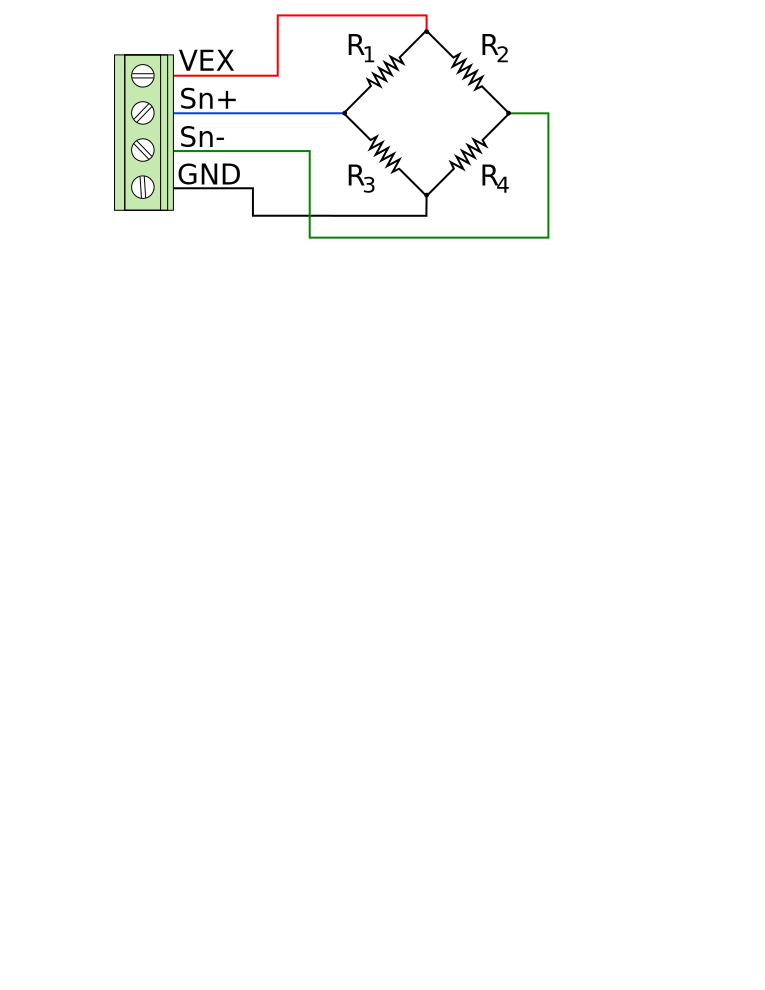
\includegraphics{strain_bridge_connections.png}}
\end{DoxyImageNoCaption}
\hypertarget{pd_sensors_sg_details}{}\subsection{Details}\label{pd_sensors_sg_details}
Strain gauges must be connected in a Wheatstone bridge circuit, and the bridge must be built entirely by the user. There are no brige completion resistors on the Poly\-D\-A\-Q board. Strain gauges and resistors of any resistance from 120 ohms to 1000 ohms may be used, as long as all the resistances are the same within a given bridge. 350 ohm gauges are preferred, as they give a good balance between low power usage (for which higher resistance gauges are better) and low noise (for which lower resistance gauges are better). If plain resistors are used to complete a quarter-\/ or half-\/bridge, precision resistors of 1\% or better tolerance are recommended.

Before connecting a strain gauge bridge to the Poly\-D\-A\-Q 2, connect all four resistances in the bridge (be they active gauges, dummy gauges, or resistors) and use an ohmmeter to check the resistances between the corners of the bridge. The resistance between opposite bridge corners should be equal to the resistance of each gauge or resistor. The resistance between adjacent corners (across each one resistance) should be 3/4 of the resistance of one resistor when that resistor was out of the bridge. If the bridge resistances are not within 1\% of the values they should have, {\ttfamily do} {\ttfamily not} connect the bridge to the Poly\-D\-A\-Q; it will be impossible to balance and won't work. Fix the bridge and {\itshape then} connect it. {\bfseries Note\-:} Do not attempt to measure bridge resistances after connecting the bridge to the Poly\-D\-A\-Q board; always disconnect the bridge from the board before measuring resistances.

The four \char`\"{}corners\char`\"{} of the bridge are connected to a set of four adjacent terminals {\ttfamily V\-E\-X}, {\ttfamily Sn+}, {\ttfamily Sn-\/}, and {\ttfamily G\-N\-D} on the Poly\-D\-A\-Q. The {\ttfamily V\-E\-X} terminal is the excitation voltage, which is controlled by the board's onboard regulator at 3.\-3\-V. The {\ttfamily Sn+} and {\ttfamily Sn-\/} terminals (replace the letter {\ttfamily n} with the bridge number) connect to the Wheatstone bridge's outputs, which are sometimes referred to as the bridge's {\ttfamily A} and {\ttfamily B} outputs on documentation. The {\ttfamily G\-N\-D} connection is of course ground.\hypertarget{pd_sensors_sss_sg_bal}{}\subsubsection{Balancing Strain Gauge Bridges}\label{pd_sensors_sss_sg_bal}
Each Poly\-D\-A\-Q 2 has two strain gauge bridges which can be automatically balanced. There are two auto-\/balanced bridges because the S\-T\-M32\-F405\-V\-G microcontroller has two D/\-A converters which are used for the balancing. On boards with four bridge amplifiers, two of the bridges use manual balancing potentiometers which are discussed below.

The {\bfseries auto-\/balancer} can be operated from the Poly\-D\-A\-Q G\-U\-I or a terminal. The G\-U\-I is documented in its own section of this manual. When communicating with a Poly\-D\-A\-Q 2 through a dumb terminal, the strain bridge auto-\/balancer is invoked by the commands {\bfseries L} and {\bfseries M} for the first and second bridges respectively. A message will be shown in the terminal telling if the auto-\/balancing was successful. If there is a problem with the bridge resistances (usually, one resistance is missing or a connection is bad) the bridge cannot be balanced. The bridge must be disconnected from the Poly\-D\-A\-Q and re-\/checked with an ohmmeter. When the problem has been solved, reconnect the bridge and auto-\/balancing should be successful.

The {\bfseries manual} {\bfseries balancer} is operated by turning the adjustment screws on each of the two bridge balancing potentiometers marked {\ttfamily B\-A\-L\-\_\-3} and {\ttfamily B\-A\-L\-\_\-4}. The potentiometers are blue colored rectangular boxes near the {\ttfamily S3} and {\ttfamily S4} inputs on the terminal blocks. Use a voltmeter ({\bfseries not} an oscilloscope) to measure the voltage at the {\ttfamily S3} or {\ttfamily S4} test point near the edge of the Poly\-D\-A\-Q board. With the strain gauge at its zero-\/strain or equilibrium position, turn the potentiometer screw for the appropriate channel so that the voltage at the {\ttfamily S3} or {\ttfamily S4} test point becomes about 1.\-67 volts. This will set the A/\-D output to about half its full scale so that both positive and negative strains can be measured. If you need the maximum range and resolution possible from the bridge amplifier, you can adjust the potentiometer so that the amplifier output voltage at the {\ttfamily S3} or {\ttfamily S4} test point is close to zero, though a zero-\/strain reading of exactly zero volts is not recommended because it will make a drift of the zero point to voltages below zero undetectable. After you've adjusted the gain potentiometer, apply some positive load to the device being tested (if possible) and verify that the amplifier output voltage is going in the right direction. If it is going the wrong way, reversing the Wheatstone bridge output connections to the {\ttfamily Sn+} and {\ttfamily Sn-\/} terminals and re-\/zeroing the bridge will cause positive strains to register as positive voltages.\hypertarget{pd_sensors_sg_calib}{}\subsubsection{Calibration}\label{pd_sensors_sg_calib}
The excitation voltage for the strain gauges is nominally 3.\-3 volts. For the best accuracy, you can measure the excitation voltage when all your strain gauges are connected and the Poly\-D\-A\-Q 2 is using the same power supply (such as a particular laptop's U\-S\-B connection) that is used during your tests. Make sure to use an accurate voltmeter set to the range which gives the most resolution. Each strain gauge bridge amplifier has a gain of 100.\-2 $\pm$ 0.\-5\%. The bridge output goes directly to the 12-\/bit A/\-D converter's input, and the A/\-D converter's reference voltage is supplied by a high-\/accuracy 3.\-3 volt reference source (L\-T1460) whose accuracy rating is better than 0.\-1\%.\hypertarget{pd_sensors_sec_vin}{}\section{Voltage Inputs}\label{pd_sensors_sec_vin}
\hypertarget{pd_sensors_ss_vin_steps}{}\subsection{Steps}\label{pd_sensors_ss_vin_steps}

\begin{DoxyEnumerate}
\item Ensure that your voltage source produces at least 0.\-5 volts or so of output when your maximum signal is being measured and that it has a negative output or common ground that can be connected to the Poly\-D\-A\-Q's ground.
\item Ensure that you can power the sensor from the Poly\-D\-A\-Q's 3.\-3 volt excitation voltage ({\ttfamily V\-E\-X} terminals). If not, find an appropriate power supply for your sensor. The power supply's ground must be attached to the Poly\-D\-A\-Q's ground. In any case, sensors whose output is greater than $\pm$ 10 volts should not be used.
\item If the sensor's output will always be in the range of 0 -- 3.\-3 volts, connect the sensor's output to the board's {\ttfamily V\-\_\-3} or {\ttfamily V\-\_\-4} input if you have a Poly\-D\-A\-Q 0-\/4-\/4 board, or any voltage input for a Poly\-D\-A\-Q 4-\/4-\/2 board.
\item If the sensor's output is larger but in the range of -\/10 to +10 volts, connect it to the {\ttfamily V\-\_\-1} or {\ttfamily V\-\_\-2} input of a Poly\-D\-A\-Q 0-\/4-\/4 board or any voltage input of a Poly\-D\-A\-Q 4-\/4-\/2 board.
\item Check that the calibration of voltage inputs is correct using a high accuracy voltmeter (not the \$4.\-00 kind).
\end{DoxyEnumerate}\hypertarget{pd_sensors_ss_vin_det}{}\subsection{Details}\label{pd_sensors_ss_vin_det}
The Poly\-D\-A\-Q 2 has two types of voltage inputs, with different configurations of the board using different combinations thereof\-:
\begin{DoxyItemize}
\item  $\pm$ 10 volt inputs. These inputs use a voltage divider and level shifter circuit to convert signals in the range of approximately -\/10 to 10 volts into signals in the range 0 -- 3.\-3 volts, which are measured by the A/\-D converter. If the inputs are disconnected, the A/\-D converter will return a reading of about 2048, or halfway between the minimum and maximum. Connecting these inputs to ground should produce an A/\-D output of about 1726.
\item 0 -- 3.\-3 volt inputs. These inputs All the voltage inputs are single-\/ended; that is, all are referenced to ground. Differential voltage measurements must be made using an external differential amplifier or, for small enough differences, the strain gauge bridge amplifiers as described in the \hyperlink{pd_sensors_sec_mV}{Millivolt Inputs} section.
\end{DoxyItemize}

For best accuracy, voltage inputs should be calibrated against a high-\/accuracy voltmeter. The resistors used to divide and shift $\pm$ 10 volt signals into the 0 -- 3.\-3 volt signals read by the analog to digital converter are not especially high accuracy resistors, so the gains of individual Poly\-D\-A\-Q boards may vary by up to about 3\%. The 0 -- 3.\-3\-V inputs should be accurate to within better than 0.\-5\% as long as input impedance is not a problem.

 $\pm$ 10 volt inputs have an input impedance of approximately 220\-K $\Omega$. This means that they can be used to measure signals from amplified transducers without loading the measured signals, but low-\/energy signals such as those from piezoelectric, capacitive, thermocouple, and biological sensors must be amplified by proper signal conditioning amplifiers before being sent to the Poly\-D\-A\-Q's voltage inputs.

0 -- 3.\-3 volt inputs have an input impedance of approximately 300\-K $\Omega$ and are subject to the same considerations of source impedance as the $\pm$ 10 volt inputs. Although these inputs are somewhat protected from excessive voltages by series resistors at their inputs, care must be taken to prevent voltages outside the range 0 -- 3.\-3 volts from being connected to these inputs.\hypertarget{pd_sensors_sec_pot}{}\subsubsection{Potentiometers}\label{pd_sensors_sec_pot}
Using a potentiometer as a position transducer is especially easy.
\begin{DoxyEnumerate}
\item Choose a potentiometer whose resistance is 1\-K $\Omega$ to 10\-K $\Omega$, and make sure it has a \char`\"{}linear taper\char`\"{} (linear relationship between angle or distance and resistance change).
\item Connect one end of the potentiometer to the +3.3\-V source at a terminal marked {\ttfamily V\-E\-X}.
\item Connect the other end of the potentiometer to a ground terminal.
\item Connect the potentiometer's center terminal, the one for the moving \char`\"{}wiper\char`\"{}, to a voltage input (on a Poly\-D\-A\-Q 0-\/4-\/4, inputs {\ttfamily V\-\_\-3} and {\ttfamily V\-\_\-4} will give the best resolution).
\item Run the Poly\-D\-A\-Q G\-U\-I or a dumb terminal to test and calibrate the position to voltage transducer. See \hyperlink{pd_channels}{Channel Commands} for a list of commands to get data from each A/\-D channel.
\end{DoxyEnumerate}\hypertarget{pd_sensors_sec_mV}{}\subsubsection{Millivolt Inputs}\label{pd_sensors_sec_mV}
If you need to measure a small difference between voltages which are both in the range 0 -\/ 3.\-3\-V from ground, you can use a strain gauge bridge amplifier as a differential amplifier with a gain of about 100. It is best to protect the amplifier's inputs by placing 100 $\Omega$ resistors in series with the voltage source, unless the excitation voltage and ground are used to power the sensors (as they are with strain gauge bridges). If both inputs \char`\"{}float\char`\"{} with respect to ground (such as with self-\/powering sensors such as thermocouples), use a 100\-K $\Omega$ to 1\-M $\Omega$ resistor between the {\ttfamily Sn-\/} input and ground to ensure that the signals both remain within the measurable range of 0 to 3.\-3 volts.\hypertarget{pd_sensors_sec_accel}{}\section{Accelerometers}\label{pd_sensors_sec_accel}
\hypertarget{pd_sensors_ss_onb_accel}{}\subsection{The Onboard Accelerometer}\label{pd_sensors_ss_onb_accel}
The Poly\-D\-A\-Q 0-\/4-\/4 has an accelerometer on the board. This accelerometer, a Freescale M\-M\-A8452\-Q, is a modern micromachined electromechanical system (M\-E\-M\-S) device. It sends data in digital form over an I2\-C bus. It can measure 3 axes of accelerations with 12-\/bit resolution and a full-\/scale reading of  $\pm$ 2 g, $\pm$ 4 g, or $\pm$ 8 g; the accelerometer is normally set to read $\pm$ 2 g. There are white printed arrows on the board showing the directions of the X, Y, and Z axes as measured. There are no connections needed to use the onboard accelerometer. Set the Python G\-U\-I to read the accelerometer, or use channel commands {\ttfamily X}, {\ttfamily Y}, and/or {\ttfamily Z} (note that these are {\itshape uppercase} letters) in the data logger configuration file (see section \hyperlink{pd_setup_pds_sd_config}{The Configuration File}). Accelerometer data can be taken at up to 200 samples per second.\hypertarget{pd_sensors_ss_ext_accel}{}\subsection{An External Accelerometer}\label{pd_sensors_ss_ext_accel}
An external accelerometer, also a M\-M\-A8452\-Q, can be connected to the I2\-C connector which is located next to the black power jack near one corner of the board. The external accelerometer will be mounted to a \char`\"{}breakout board\char`\"{}, a small circuit board with connections that are labeled {\ttfamily 3.\-3\-V}, {\ttfamily S\-C\-L}, {\ttfamily S\-D\-A}, and {\ttfamily G\-N\-D}. The four pins of the I2\-C connector are labeled {\ttfamily 3\-V3}, {\ttfamily S\-C\-L}, {\ttfamily S\-D\-A}, and {\ttfamily G\-N\-D}, going from farthest to closest to the power jack. (Connections {\ttfamily I1} and {\ttfamily I2} on the breakout board need not be connected.) Turn the Poly\-D\-A\-Q's power off; connect the matching connections on the breakout board to those on the Poly\-D\-A\-Q's connector; turn power back on, and the external accelerometer will be ready to use. The external accelerometer responds to lowercase versions of the internal accelerometer's commands, returning data when queried with {\ttfamily x}, {\ttfamily y}, and {\ttfamily z}.

 
\begin{DoxyImageNoCaption}
  \mbox{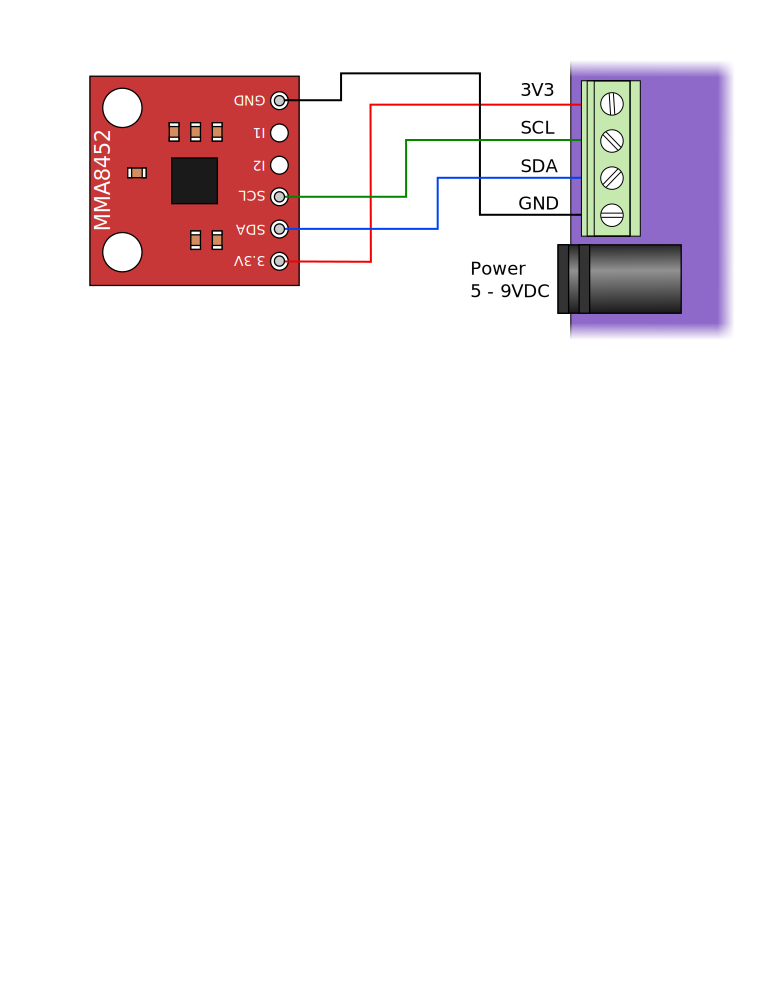
\includegraphics{ext_accel_connections_small.png}}
\end{DoxyImageNoCaption}
\hypertarget{pd_sensors_ss_ana_accel}{}\subsection{Analog Accelerometers}\label{pd_sensors_ss_ana_accel}
Other types of external accelerometers which use analog signals rather than digital ones can be connected directly to the voltage inputs of the Poly\-D\-A\-Q. No special considerations need necessarily be applied when using such accelerometers, except that the accelerometers should be compatible with the 3.\-3 volt power supplied by the Poly\-D\-A\-Q 2 board, and that power can be connected to the accelerometers by using the {\ttfamily V\-E\-X} connections for the strain gauges and the {\ttfamily G\-N\-D} connections next to the voltage inputs.\hypertarget{pd_sensors_sec_thorno}{}\section{Thermocouple Inputs}\label{pd_sensors_sec_thorno}
Who uses {\itshape those} things? 
\chapter{Hierarchical Index}
\section{Class Hierarchy}
This inheritance list is sorted roughly, but not completely, alphabetically\-:\begin{DoxyCompactList}
\item \contentsline{section}{config\-\_\-file}{\pageref{classconfig__file}}{}
\item \contentsline{section}{logger\-\_\-col\-\_\-cfg}{\pageref{classlogger__col__cfg}}{}
\item \contentsline{section}{logger\-\_\-config}{\pageref{classlogger__config}}{}
\item \contentsline{section}{polydaq2}{\pageref{classpolydaq2}}{}
\item Task\-Base\begin{DoxyCompactList}
\item \contentsline{section}{task\-\_\-data\-\_\-acq}{\pageref{classtask__data__acq}}{}
\item \contentsline{section}{task\-\_\-leds}{\pageref{classtask__leds}}{}
\item \contentsline{section}{task\-\_\-pc}{\pageref{classtask__pc}}{}
\item \contentsline{section}{task\-\_\-print}{\pageref{classtask__print}}{}
\item \contentsline{section}{task\-\_\-sd\-\_\-card}{\pageref{classtask__sd__card}}{}
\item \contentsline{section}{task\-\_\-sd\-\_\-daq}{\pageref{classtask__sd__daq}}{}
\item \contentsline{section}{task\-\_\-user}{\pageref{classtask__user}}{}
\end{DoxyCompactList}
\end{DoxyCompactList}

\chapter{Class Index}
\section{Class List}
Here are the classes, structs, unions and interfaces with brief descriptions\-:\begin{DoxyCompactList}
\item\contentsline{section}{\hyperlink{classconfig__file}{config\-\_\-file} \\*Base class for a configuration file reader and parser }{\pageref{classconfig__file}}{}
\item\contentsline{section}{\hyperlink{classlogger__col__cfg}{logger\-\_\-col\-\_\-cfg} \\*Data for one sensor line in the logger configuration file }{\pageref{classlogger__col__cfg}}{}
\item\contentsline{section}{\hyperlink{classlogger__config}{logger\-\_\-config} \\*Parser for simple data logger configuration files }{\pageref{classlogger__config}}{}
\item\contentsline{section}{\hyperlink{classpolydaq2}{polydaq2} \\*Class which interacts with Poly\-D\-A\-Q 2 hardware }{\pageref{classpolydaq2}}{}
\item\contentsline{section}{\hyperlink{classtask__data__acq}{task\-\_\-data\-\_\-acq} \\*Task which acquires Poly\-D\-A\-Q data at precise time intervals }{\pageref{classtask__data__acq}}{}
\item\contentsline{section}{\hyperlink{classtask__leds}{task\-\_\-leds} \\*Task which pulses an L\-E\-D on and off as another responds to a button }{\pageref{classtask__leds}}{}
\item\contentsline{section}{\hyperlink{classtask__pc}{task\-\_\-pc} \\*Task for communication with the user or a P\-C based user interface }{\pageref{classtask__pc}}{}
\item\contentsline{section}{\hyperlink{classtask__print}{task\-\_\-print} \\*Task which prints out characters in the main print queue }{\pageref{classtask__print}}{}
\item\contentsline{section}{\hyperlink{classtask__sd__card}{task\-\_\-sd\-\_\-card} \\*Task which saves data to an S\-D card }{\pageref{classtask__sd__card}}{}
\item\contentsline{section}{\hyperlink{classtask__sd__daq}{task\-\_\-sd\-\_\-daq} \\*Task which acquires Poly\-D\-A\-Q data for the S\-D card }{\pageref{classtask__sd__daq}}{}
\item\contentsline{section}{\hyperlink{classtask__user}{task\-\_\-user} \\*Task for communication with the user or a P\-C based user interface }{\pageref{classtask__user}}{}
\end{DoxyCompactList}

\chapter{File Index}
\section{File List}
Here is a list of all documented files with brief descriptions\-:\begin{DoxyCompactList}
\item\contentsline{section}{\hyperlink{appconfig_8h}{appconfig.\-h} }{\pageref{appconfig_8h}}{}
\item\contentsline{section}{\hyperlink{config__file_8cpp}{config\-\_\-file.\-cpp} \\*Source code for a base class for small program configuration files }{\pageref{config__file_8cpp}}{}
\item\contentsline{section}{\hyperlink{config__file_8h}{config\-\_\-file.\-h} \\*Header for a base class for small program configuration files }{\pageref{config__file_8h}}{}
\item\contentsline{section}{\hyperlink{FreeRTOSConfig_8h}{Free\-R\-T\-O\-S\-Config.\-h} \\*Configuration settings for Free\-R\-T\-O\-S as it's used in this project }{\pageref{FreeRTOSConfig_8h}}{}
\item\contentsline{section}{\hyperlink{logger__config_8cpp}{logger\-\_\-config.\-cpp} \\*Source code for a parser for data logging configuration files }{\pageref{logger__config_8cpp}}{}
\item\contentsline{section}{\hyperlink{logger__config_8h}{logger\-\_\-config.\-h} \\*Headers for a parser for data logging configuration files }{\pageref{logger__config_8h}}{}
\item\contentsline{section}{\hyperlink{main_8cpp}{main.\-cpp} \\*The main file for the Poly\-D\-A\-Q 2 firmware }{\pageref{main_8cpp}}{}
\item\contentsline{section}{\hyperlink{polydaq2_8cpp}{polydaq2.\-cpp} }{\pageref{polydaq2_8cpp}}{}
\item\contentsline{section}{\hyperlink{polydaq2_8h}{polydaq2.\-h} \\*Headers for a class that drives the Poly\-D\-A\-Q 2 board's hardware }{\pageref{polydaq2_8h}}{}
\item\contentsline{section}{\hyperlink{shares_8h}{shares.\-h} \\*Declarations for inter-\/task data communication items (shares and queues) }{\pageref{shares_8h}}{}
\item\contentsline{section}{\hyperlink{task__data__acq_8cpp}{task\-\_\-data\-\_\-acq.\-cpp} }{\pageref{task__data__acq_8cpp}}{}
\item\contentsline{section}{\hyperlink{task__data__acq_8h}{task\-\_\-data\-\_\-acq.\-h} }{\pageref{task__data__acq_8h}}{}
\item\contentsline{section}{\hyperlink{task__leds_8cpp}{task\-\_\-leds.\-cpp} }{\pageref{task__leds_8cpp}}{}
\item\contentsline{section}{\hyperlink{task__leds_8h}{task\-\_\-leds.\-h} }{\pageref{task__leds_8h}}{}
\item\contentsline{section}{\hyperlink{task__pc_8cpp}{task\-\_\-pc.\-cpp} }{\pageref{task__pc_8cpp}}{}
\item\contentsline{section}{\hyperlink{task__pc_8h}{task\-\_\-pc.\-h} }{\pageref{task__pc_8h}}{}
\item\contentsline{section}{\hyperlink{task__sd__card_8cpp}{task\-\_\-sd\-\_\-card.\-cpp} \\*Source code for a task which saves data to an S\-D card }{\pageref{task__sd__card_8cpp}}{}
\item\contentsline{section}{\hyperlink{task__sd__card_8h}{task\-\_\-sd\-\_\-card.\-h} \\*Headers for a task which saves data to an S\-D card }{\pageref{task__sd__card_8h}}{}
\item\contentsline{section}{\hyperlink{task__sd__daq_8cpp}{task\-\_\-sd\-\_\-daq.\-cpp} }{\pageref{task__sd__daq_8cpp}}{}
\item\contentsline{section}{\hyperlink{task__sd__daq_8h}{task\-\_\-sd\-\_\-daq.\-h} }{\pageref{task__sd__daq_8h}}{}
\item\contentsline{section}{\hyperlink{task__user_8cpp}{task\-\_\-user.\-cpp} }{\pageref{task__user_8cpp}}{}
\item\contentsline{section}{\hyperlink{task__user_8h}{task\-\_\-user.\-h} }{\pageref{task__user_8h}}{}
\end{DoxyCompactList}

\chapter{Class Documentation}
\hypertarget{classconfig__file}{\section{config\-\_\-file Class Reference}
\label{classconfig__file}\index{config\-\_\-file@{config\-\_\-file}}
}


Base class for a configuration file reader and parser.  




{\ttfamily \#include $<$config\-\_\-file.\-h$>$}

\subsection*{Public Member Functions}
\begin{DoxyCompactItemize}
\item 
\hyperlink{classconfig__file_ac2724c3ca140fd2932cb956d0f06e315}{config\-\_\-file} (sd\-\_\-card $\ast$p\-\_\-sd\-\_\-card, emstream $\ast$p\-\_\-ser\-\_\-dev)
\begin{DoxyCompactList}\small\item\em Constructor for a base configuration file parser. \end{DoxyCompactList}\item 
virtual void \hyperlink{classconfig__file_a55798c93bc529cfa7d79e199f1ad7925}{read} (char const $\ast$)
\begin{DoxyCompactList}\small\item\em Read a configuration file, parsing each line to find settings. \end{DoxyCompactList}\item 
int16\-\_\-t \hyperlink{classconfig__file_aa0c5fee1c2a104dd501f4499b526b184}{skip\-\_\-to\-\_\-next\-\_\-line} (void)
\begin{DoxyCompactList}\small\item\em Skip whitespace characters and comments until data is found. \end{DoxyCompactList}\item 
void \hyperlink{classconfig__file_a05bfc7892289bec6441710bf7f2c092b}{skip\-\_\-to\-\_\-\-E\-O\-L} (void)
\begin{DoxyCompactList}\small\item\em Skip from a comment delimiter character to the end of a line. \end{DoxyCompactList}\item 
uint8\-\_\-t \hyperlink{classconfig__file_a672af5504446db5f89896aada5980468}{read\-\_\-bool} (uint16\-\_\-t)
\begin{DoxyCompactList}\small\item\em Read one boolean value from a configuration file. \end{DoxyCompactList}\end{DoxyCompactItemize}
\subsection*{Protected Attributes}
\begin{DoxyCompactItemize}
\item 
sd\-\_\-card $\ast$ \hyperlink{classconfig__file_a7f5e8d1a7a4b760531853d43857fc527}{p\-\_\-card}
\begin{DoxyCompactList}\small\item\em A pointer to the S\-D card driver. \end{DoxyCompactList}\item 
emstream $\ast$ \hyperlink{classconfig__file_a529cb0760d01190b93076cb9e7da4746}{p\-\_\-serial}
\begin{DoxyCompactList}\small\item\em Pointer to a serial device used for debugging messages. \end{DoxyCompactList}\end{DoxyCompactItemize}


\subsection{Detailed Description}
Base class for a configuration file reader and parser. 

This class parses a configuration file which is kept on some type of serially accessed device such as an S\-D card. The configuration file is made up in sections, with sections being indicated by a text header in brackets; the file contains items which map to variables that will be kept in the configuration, generally numbers and flags (boolean values) and, in the future, perhaps text strings and comments. The items are distinguished as follows\-: \begin{DoxyItemize}
\item Comments are put in the file line by line; they begin with a number sign ({\ttfamily \#}). When a number sign is found, the rest of the line is ignored. A comment may be on a line after a data item. \item Numbers are expected to be integers (floats may be supported in the future). They are given one per line. It's O\-K to have comments after the numbers. \item Boolean values can be given as text which begins with {\ttfamily Y}, {\ttfamily y}, {\ttfamily T}, {\ttfamily t}, or {\ttfamily On} for values which are true; {\ttfamily N}, {\ttfamily n}, {\ttfamily F}, {\ttfamily f}, and {\ttfamily Off} represent false values.\end{DoxyItemize}
An example file looks like the following\-: 
\begin{DoxyCode}
\textcolor{preprocessor}{# Sample configuration file}
\textcolor{preprocessor}{}\textcolor{preprocessor}{# This comment explains something really important.}
\textcolor{preprocessor}{}157            # Numerator
100            # Denominator
-13            # Offset

\textcolor{preprocessor}{# End of file}
\end{DoxyCode}
 

Definition at line 94 of file config\-\_\-file.\-h.



\subsection{Constructor \& Destructor Documentation}
\hypertarget{classconfig__file_ac2724c3ca140fd2932cb956d0f06e315}{\index{config\-\_\-file@{config\-\_\-file}!config\-\_\-file@{config\-\_\-file}}
\index{config\-\_\-file@{config\-\_\-file}!config_file@{config\-\_\-file}}
\subsubsection[{config\-\_\-file}]{\setlength{\rightskip}{0pt plus 5cm}config\-\_\-file\-::config\-\_\-file (
\begin{DoxyParamCaption}
\item[{sd\-\_\-card $\ast$}]{p\-\_\-sd\-\_\-card, }
\item[{emstream $\ast$}]{p\-\_\-ser\-\_\-dev}
\end{DoxyParamCaption}
)}}\label{classconfig__file_ac2724c3ca140fd2932cb956d0f06e315}


Constructor for a base configuration file parser. 

This constructor creates the base class portion of a configuration file parser which reads files on a given serial decice. 
\begin{DoxyParams}{Parameters}
{\em p\-\_\-sd\-\_\-card} & Pointer to a device such as an S\-D card on which the file is kept \\
\hline
{\em p\-\_\-ser\-\_\-dev} & Serial device (such as a port) on which to show debugging information \\
\hline
\end{DoxyParams}


Definition at line 45 of file config\-\_\-file.\-cpp.



References p\-\_\-card, and p\-\_\-serial.



\subsection{Member Function Documentation}
\hypertarget{classconfig__file_a55798c93bc529cfa7d79e199f1ad7925}{\index{config\-\_\-file@{config\-\_\-file}!read@{read}}
\index{read@{read}!config_file@{config\-\_\-file}}
\subsubsection[{read}]{\setlength{\rightskip}{0pt plus 5cm}void config\-\_\-file\-::read (
\begin{DoxyParamCaption}
\item[{char const $\ast$}]{file\-\_\-name}
\end{DoxyParamCaption}
)\hspace{0.3cm}{\ttfamily [virtual]}}}\label{classconfig__file_a55798c93bc529cfa7d79e199f1ad7925}


Read a configuration file, parsing each line to find settings. 

This is a base class method to read a configuration file. It only reads and prints out the file, if debugging is properly enabled. Descendent classes need to implement their own versions of {\ttfamily \hyperlink{classconfig__file_a55798c93bc529cfa7d79e199f1ad7925}{read()}} which are appropriate for configurations of specific systems. 
\begin{DoxyParams}{Parameters}
{\em file\-\_\-name} & Pointer to a string containing the name of the file to be read \\
\hline
\end{DoxyParams}


Definition at line 64 of file config\-\_\-file.\-cpp.



References C\-F\-G\-F\-\_\-\-D\-B\-G, and p\-\_\-card.

\hypertarget{classconfig__file_a672af5504446db5f89896aada5980468}{\index{config\-\_\-file@{config\-\_\-file}!read\-\_\-bool@{read\-\_\-bool}}
\index{read\-\_\-bool@{read\-\_\-bool}!config_file@{config\-\_\-file}}
\subsubsection[{read\-\_\-bool}]{\setlength{\rightskip}{0pt plus 5cm}uint8\-\_\-t config\-\_\-file\-::read\-\_\-bool (
\begin{DoxyParamCaption}
\item[{uint16\-\_\-t}]{a\-\_\-char}
\end{DoxyParamCaption}
)}}\label{classconfig__file_a672af5504446db5f89896aada5980468}


Read one boolean value from a configuration file. 

This method reads a Boolean value from the configuration file. The value may be represented by various symbols; anything beginning with {\ttfamily }\mbox{[}Yy\-Tt\mbox{]} is taken as meaning true; anything beginning with {\ttfamily }\mbox{[}Nn\-Ff\mbox{]} is taken as false; if the first letter is {\ttfamily }\mbox{[}Oo\mbox{]} then the second letter is checked, as we've probably got {\ttfamily On} or {\ttfamily Off}. 
\begin{DoxyParams}{Parameters}
{\em a\-\_\-char} & The first character of the item, often found by \hyperlink{classconfig__file_aa0c5fee1c2a104dd501f4499b526b184}{skip\-\_\-to\-\_\-next\-\_\-line()} \\
\hline
\end{DoxyParams}
\begin{DoxyReturn}{Returns}
0 for false, 1 for true, and 0x\-F\-F for undetermined (not a valid Boolean) 
\end{DoxyReturn}


Definition at line 171 of file config\-\_\-file.\-cpp.



References p\-\_\-card.

\hypertarget{classconfig__file_a05bfc7892289bec6441710bf7f2c092b}{\index{config\-\_\-file@{config\-\_\-file}!skip\-\_\-to\-\_\-\-E\-O\-L@{skip\-\_\-to\-\_\-\-E\-O\-L}}
\index{skip\-\_\-to\-\_\-\-E\-O\-L@{skip\-\_\-to\-\_\-\-E\-O\-L}!config_file@{config\-\_\-file}}
\subsubsection[{skip\-\_\-to\-\_\-\-E\-O\-L}]{\setlength{\rightskip}{0pt plus 5cm}void config\-\_\-file\-::skip\-\_\-to\-\_\-\-E\-O\-L (
\begin{DoxyParamCaption}
\item[{void}]{}
\end{DoxyParamCaption}
)}}\label{classconfig__file_a05bfc7892289bec6441710bf7f2c092b}


Skip from a comment delimiter character to the end of a line. 

This method is called when a comment character has been found. It reads and ignores all characters up to the end of the current line. The file pointer is moved forward in the file, but nothing else is changed. 

Definition at line 151 of file config\-\_\-file.\-cpp.



References C\-F\-G\-\_\-\-E\-N\-D\-\_\-\-O\-F\-\_\-\-L\-I\-N\-E, and p\-\_\-card.



Referenced by skip\-\_\-to\-\_\-next\-\_\-line().

\hypertarget{classconfig__file_aa0c5fee1c2a104dd501f4499b526b184}{\index{config\-\_\-file@{config\-\_\-file}!skip\-\_\-to\-\_\-next\-\_\-line@{skip\-\_\-to\-\_\-next\-\_\-line}}
\index{skip\-\_\-to\-\_\-next\-\_\-line@{skip\-\_\-to\-\_\-next\-\_\-line}!config_file@{config\-\_\-file}}
\subsubsection[{skip\-\_\-to\-\_\-next\-\_\-line}]{\setlength{\rightskip}{0pt plus 5cm}int16\-\_\-t config\-\_\-file\-::skip\-\_\-to\-\_\-next\-\_\-line (
\begin{DoxyParamCaption}
\item[{void}]{}
\end{DoxyParamCaption}
)}}\label{classconfig__file_aa0c5fee1c2a104dd501f4499b526b184}


Skip whitespace characters and comments until data is found. 

This method reads characters, skipping whitespace (spaces and returns) and ignoring lines which are comments, until it has found the first character on the next active (non-\/comment) line. That first character is returned, and the file pointer is left pointing to the character after that first character. \begin{DoxyReturn}{Returns}
The first non-\/comment character found, or (-\/1) if error or end of file 
\end{DoxyReturn}


Definition at line 102 of file config\-\_\-file.\-cpp.



References C\-F\-G\-\_\-\-C\-O\-M\-M\-E\-N\-T\-\_\-\-C\-H\-A\-R, C\-F\-G\-\_\-\-E\-N\-D\-\_\-\-O\-F\-\_\-\-L\-I\-N\-E, p\-\_\-card, and skip\-\_\-to\-\_\-\-E\-O\-L().



\subsection{Member Data Documentation}
\hypertarget{classconfig__file_a7f5e8d1a7a4b760531853d43857fc527}{\index{config\-\_\-file@{config\-\_\-file}!p\-\_\-card@{p\-\_\-card}}
\index{p\-\_\-card@{p\-\_\-card}!config_file@{config\-\_\-file}}
\subsubsection[{p\-\_\-card}]{\setlength{\rightskip}{0pt plus 5cm}sd\-\_\-card$\ast$ config\-\_\-file\-::p\-\_\-card\hspace{0.3cm}{\ttfamily [protected]}}}\label{classconfig__file_a7f5e8d1a7a4b760531853d43857fc527}


A pointer to the S\-D card driver. 

This pointer points to the S\-D card driver which is used to access the configuration file. 

Definition at line 101 of file config\-\_\-file.\-h.



Referenced by config\-\_\-file(), read(), read\-\_\-bool(), skip\-\_\-to\-\_\-\-E\-O\-L(), and skip\-\_\-to\-\_\-next\-\_\-line().

\hypertarget{classconfig__file_a529cb0760d01190b93076cb9e7da4746}{\index{config\-\_\-file@{config\-\_\-file}!p\-\_\-serial@{p\-\_\-serial}}
\index{p\-\_\-serial@{p\-\_\-serial}!config_file@{config\-\_\-file}}
\subsubsection[{p\-\_\-serial}]{\setlength{\rightskip}{0pt plus 5cm}emstream$\ast$ config\-\_\-file\-::p\-\_\-serial\hspace{0.3cm}{\ttfamily [protected]}}}\label{classconfig__file_a529cb0760d01190b93076cb9e7da4746}


Pointer to a serial device used for debugging messages. 

This pointer points to a serial port which can be used for debugging. If left at {\ttfamily N\-U\-L\-L}, debugging printouts won't take place. 

Definition at line 108 of file config\-\_\-file.\-h.



Referenced by config\-\_\-file().



The documentation for this class was generated from the following files\-:\begin{DoxyCompactItemize}
\item 
\hyperlink{config__file_8h}{config\-\_\-file.\-h}\item 
\hyperlink{config__file_8cpp}{config\-\_\-file.\-cpp}\end{DoxyCompactItemize}

\hypertarget{classlogger__col__cfg}{\section{logger\-\_\-col\-\_\-cfg Class Reference}
\label{classlogger__col__cfg}\index{logger\-\_\-col\-\_\-cfg@{logger\-\_\-col\-\_\-cfg}}
}


Data for one sensor line in the logger configuration file.  




{\ttfamily \#include $<$logger\-\_\-config.\-h$>$}

\subsection*{Public Member Functions}
\begin{DoxyCompactItemize}
\item 
\hypertarget{classlogger__col__cfg_a6e7d9e299aee792b6914dcde5868ebe4}{\hyperlink{classlogger__col__cfg_a6e7d9e299aee792b6914dcde5868ebe4}{logger\-\_\-col\-\_\-cfg} (void)}\label{classlogger__col__cfg_a6e7d9e299aee792b6914dcde5868ebe4}

\begin{DoxyCompactList}\small\item\em The constructor sets default values for everything. \end{DoxyCompactList}\end{DoxyCompactItemize}
\subsection*{Public Attributes}
\begin{DoxyCompactItemize}
\item 
\hypertarget{classlogger__col__cfg_a6e82dca8f3cc2f5ad53c3596f37dee25}{char \hyperlink{classlogger__col__cfg_a6e82dca8f3cc2f5ad53c3596f37dee25}{command}}\label{classlogger__col__cfg_a6e82dca8f3cc2f5ad53c3596f37dee25}

\begin{DoxyCompactList}\small\item\em The command character which causes the Poly\-D\-A\-Q to read the channel. \end{DoxyCompactList}\item 
\hypertarget{classlogger__col__cfg_ae4b90337e551749b1be1ab3a967f8a73}{float \hyperlink{classlogger__col__cfg_ae4b90337e551749b1be1ab3a967f8a73}{slope}}\label{classlogger__col__cfg_ae4b90337e551749b1be1ab3a967f8a73}

\begin{DoxyCompactList}\small\item\em The slope for converting raw data to what is saved. \end{DoxyCompactList}\item 
\hypertarget{classlogger__col__cfg_a386fa258ee9c035dcd67bebc44789899}{float \hyperlink{classlogger__col__cfg_a386fa258ee9c035dcd67bebc44789899}{offset}}\label{classlogger__col__cfg_a386fa258ee9c035dcd67bebc44789899}

\begin{DoxyCompactList}\small\item\em The offset for converting the scaled data to what is saved. \end{DoxyCompactList}\item 
\hypertarget{classlogger__col__cfg_af82115d776b995020e0afd8061fcfa5a}{char $\ast$ \hyperlink{classlogger__col__cfg_af82115d776b995020e0afd8061fcfa5a}{p\-\_\-label}}\label{classlogger__col__cfg_af82115d776b995020e0afd8061fcfa5a}

\begin{DoxyCompactList}\small\item\em The label (name) of the given column of data. \end{DoxyCompactList}\item 
\hypertarget{classlogger__col__cfg_adec0e9660a87545cefd316a0c99b9bc5}{\hyperlink{classlogger__col__cfg}{logger\-\_\-col\-\_\-cfg} $\ast$ \hyperlink{classlogger__col__cfg_adec0e9660a87545cefd316a0c99b9bc5}{p\-\_\-next}}\label{classlogger__col__cfg_adec0e9660a87545cefd316a0c99b9bc5}

\begin{DoxyCompactList}\small\item\em Pointer to the next configuration, or {\ttfamily N\-U\-L\-L} if this is the last one. \end{DoxyCompactList}\end{DoxyCompactItemize}


\subsection{Detailed Description}
Data for one sensor line in the logger configuration file. 

This structure holds the data which is read from a single line of the logger configuration file. Each line configures one sensor with the following data\-:

\begin{TabularC}{2}
\hline
\rowcolor{lightgray}{\bf Item }&{\bf Description  }\\\cline{1-2}
Command &A one-\/character command that causes logging of this channel \\\cline{1-2}
Slope &The slope for conversions from raw data to what is saved \\\cline{1-2}
Offset &The number added to the scaled (by slope) data before saving \\\cline{1-2}
\end{TabularC}
This class is used as a simple data structure, so its data is public and methods aren't needed. 

Definition at line 82 of file logger\-\_\-config.\-h.



The documentation for this class was generated from the following file\-:\begin{DoxyCompactItemize}
\item 
\hyperlink{logger__config_8h}{logger\-\_\-config.\-h}\end{DoxyCompactItemize}

\hypertarget{classlogger__config}{\section{logger\-\_\-config Class Reference}
\label{classlogger__config}\index{logger\-\_\-config@{logger\-\_\-config}}
}


Parser for simple data logger configuration files.  




{\ttfamily \#include $<$logger\-\_\-config.\-h$>$}

\subsection*{Public Member Functions}
\begin{DoxyCompactItemize}
\item 
\hyperlink{classlogger__config_acd6780a9ad347c4adedf2fe2ceb22757}{logger\-\_\-config} (sd\-\_\-card $\ast$p\-\_\-sdc, emstream $\ast$p\-\_\-ser\-\_\-dev)
\begin{DoxyCompactList}\small\item\em Construct a logger configuration file reader object. \end{DoxyCompactList}\item 
void \hyperlink{classlogger__config_a79c7dfd8b1fc2058724e0e0cb4b22ddb}{read} (char const $\ast$file\-\_\-name)
\begin{DoxyCompactList}\small\item\em Read a data logger configuration file and figure out what it means. \end{DoxyCompactList}\item 
bool \hyperlink{classlogger__config_a6bc93719808abe5135dc4abf8656f4b7}{read\-\_\-line} (void)
\begin{DoxyCompactList}\small\item\em Read one line from the configuration file and respond to it. \end{DoxyCompactList}\item 
void \hyperlink{classlogger__config_aeb468fb4654befe3e07c993760ed5d74}{read\-\_\-channel\-\_\-config} (void)
\begin{DoxyCompactList}\small\item\em Read a channel configuration line from the configuration file. \end{DoxyCompactList}\item 
void \hyperlink{classlogger__config_a30f5e9607e7207984ab80ecba9ffcdf4}{clear} (void)
\begin{DoxyCompactList}\small\item\em Clear the logger configuration so that it can be re-\/read from scratch. \end{DoxyCompactList}\item 
uint16\-\_\-t \hyperlink{classlogger__config_a00ecb0198a63a6821bc3b22ab71707dc}{get\-\_\-ticks\-\_\-per\-\_\-sample} (void)
\begin{DoxyCompactList}\small\item\em Get the number of R\-T\-O\-S ticks per sample set. \end{DoxyCompactList}\item 
uint16\-\_\-t \hyperlink{classlogger__config_ac23329790efe715df4951a7efae8c47a}{get\-\_\-ms\-\_\-per\-\_\-sample} (void)
\begin{DoxyCompactList}\small\item\em Get the number of milliseconds per sample set. \end{DoxyCompactList}\item 
bool \hyperlink{classlogger__config_ab5a799255ee75c91aedf52132ba538df}{is\-\_\-valid} (void)
\begin{DoxyCompactList}\small\item\em Find out whether a valid configuration has been read. \end{DoxyCompactList}\item 
\hypertarget{classlogger__config_a82b78e3c8e3d361555f94aeb0ee602f2}{\hyperlink{classlogger__col__cfg}{logger\-\_\-col\-\_\-cfg} $\ast$ \hyperlink{classlogger__config_a82b78e3c8e3d361555f94aeb0ee602f2}{get\-\_\-first\-\_\-channel} (void)}\label{classlogger__config_a82b78e3c8e3d361555f94aeb0ee602f2}

\begin{DoxyCompactList}\small\item\em Return a pointer to the first channel configuration. \end{DoxyCompactList}\item 
\hypertarget{classlogger__config_a1690a900cb93b0254085ef9eb76ddc45}{\hyperlink{classlogger__col__cfg}{logger\-\_\-col\-\_\-cfg} $\ast$ \hyperlink{classlogger__config_a1690a900cb93b0254085ef9eb76ddc45}{get\-\_\-next\-\_\-channel} (void)}\label{classlogger__config_a1690a900cb93b0254085ef9eb76ddc45}

\begin{DoxyCompactList}\small\item\em Return a pointer to the next channel configuration in the list. \end{DoxyCompactList}\end{DoxyCompactItemize}
\subsection*{Protected Attributes}
\begin{DoxyCompactItemize}
\item 
sd\-\_\-card $\ast$ \hyperlink{classlogger__config_ab9beda58d9d147e75ce85b3b8024cc20}{p\-\_\-card}
\begin{DoxyCompactList}\small\item\em A pointer to the S\-D card driver. \end{DoxyCompactList}\item 
emstream $\ast$ \hyperlink{classlogger__config_ab21ca3930913e75c8e4c6cc2163f4bd7}{p\-\_\-serial}
\begin{DoxyCompactList}\small\item\em Pointer to a serial device used for debugging messages. \end{DoxyCompactList}\item 
uint16\-\_\-t \hyperlink{classlogger__config_a24d69cc1f5e9cea4f0d0b3cda10a0fd8}{ticks\-\_\-per\-\_\-reading}
\begin{DoxyCompactList}\small\item\em Number of R\-T\-O\-S ticks per sample set. \end{DoxyCompactList}\item 
uint16\-\_\-t \hyperlink{classlogger__config_aced003cf2337160be6d8288f10f116d2}{ms\-\_\-per\-\_\-reading}
\begin{DoxyCompactList}\small\item\em Number of milliseconds per sample set. \end{DoxyCompactList}\item 
\hyperlink{classlogger__col__cfg}{logger\-\_\-col\-\_\-cfg} $\ast$ \hyperlink{classlogger__config_aa522d8c1a166234b677909cea6580cf5}{p\-\_\-first\-\_\-config\-\_\-data}
\begin{DoxyCompactList}\small\item\em Pointer to the first structure of channel configuration data. \end{DoxyCompactList}\item 
\hyperlink{classlogger__col__cfg}{logger\-\_\-col\-\_\-cfg} $\ast$ \hyperlink{classlogger__config_aaf8a326ecea11b1f24a574f96fb5e52f}{p\-\_\-current\-\_\-config\-\_\-data}
\begin{DoxyCompactList}\small\item\em Pointer to the channel configuration currently being used. \end{DoxyCompactList}\item 
\hypertarget{classlogger__config_a1b17eb2e849a07d44c2846b2599d57a5}{bool \hyperlink{classlogger__config_a1b17eb2e849a07d44c2846b2599d57a5}{config\-\_\-valid}}\label{classlogger__config_a1b17eb2e849a07d44c2846b2599d57a5}

\begin{DoxyCompactList}\small\item\em This boolean is true only if a valid configuration has been read. \end{DoxyCompactList}\end{DoxyCompactItemize}
\subsection*{Friends}
\begin{DoxyCompactItemize}
\item 
\hypertarget{classlogger__config_ac45c71eed6e2714623a9ab5badf2e9e4}{emstream \& \hyperlink{classlogger__config_ac45c71eed6e2714623a9ab5badf2e9e4}{operator$<$$<$} (emstream \&str, \hyperlink{classlogger__config}{logger\-\_\-config} \&log\-\_\-cfg)}\label{classlogger__config_ac45c71eed6e2714623a9ab5badf2e9e4}

\begin{DoxyCompactList}\small\item\em Diagnostic printout of all the data from a logger configuration. \end{DoxyCompactList}\end{DoxyCompactItemize}


\subsection{Detailed Description}
Parser for simple data logger configuration files. 

This class parses simple configuration files, kept on S\-D cards, for Swoop or Poly\-D\-A\-Q 2 data loggers. Data is recorded by taking measurements from the specified channels, at the given rate in milliseconds per sample. The data is scaled by a simple linear gain and offset, then written onto the S\-D card.

The configuration file can contain the following\-: \begin{DoxyItemize}
\item Comments which describe what's in the file. A comment begins with a {\ttfamily \char`\"{}\#\char`\"{}} and lasts to the end of a line. \item Empty lines, which are ignored. \item Data lines which begin with a single letter followed by a colon. Valid data lines include\-:\end{DoxyItemize}
\begin{TabularC}{2}
\hline
\rowcolor{lightgray}\PBS\centering {\bf Letter }&{\bf Meaning  }\\\cline{1-2}
\PBS\centering H &Header line showing type of Poly\-D\-A\-Q (not used) \\\cline{1-2}
\PBS\centering B &Baud rate for serial interface to G\-U\-I (not used) \\\cline{1-2}
\PBS\centering T &Time per data sample, in milliseconds \\\cline{1-2}
\PBS\centering C &Channel configuration line, as detailed below \\\cline{1-2}
\end{TabularC}
Channel configuration lines look like the following\-: 
\begin{DoxyCode}
C: 9, 1.0, 0.0, \textcolor{stringliteral}{"Cow Strain"}
\end{DoxyCode}
 The items in the channel configuration line are as follows\-:

\begin{TabularC}{2}
\hline
\rowcolor{lightgray}\PBS\centering {\bf }&{\bf }\\\cline{1-2}
\PBS\centering {\ttfamily 9} &The single-\/letter command to read data, such as {\ttfamily 5} or {\ttfamily X} \\\cline{1-2}
\PBS\centering {\ttfamily 1.\-0} &Gain by which raw data is multiplied before being saved \\\cline{1-2}
\PBS\centering {\ttfamily 0.\-0} &Offset added to data after gain and before data is saved \\\cline{1-2}
\PBS\centering {\ttfamily \char`\"{}\-Cow Strain\char`\"{}} &Channel name written to data file as column header \\\cline{1-2}
\end{TabularC}


Definition at line 151 of file logger\-\_\-config.\-h.



\subsection{Constructor \& Destructor Documentation}
\hypertarget{classlogger__config_acd6780a9ad347c4adedf2fe2ceb22757}{\index{logger\-\_\-config@{logger\-\_\-config}!logger\-\_\-config@{logger\-\_\-config}}
\index{logger\-\_\-config@{logger\-\_\-config}!logger_config@{logger\-\_\-config}}
\subsubsection[{logger\-\_\-config}]{\setlength{\rightskip}{0pt plus 5cm}logger\-\_\-config\-::logger\-\_\-config (
\begin{DoxyParamCaption}
\item[{sd\-\_\-card $\ast$}]{p\-\_\-sd\-\_\-card, }
\item[{emstream $\ast$}]{p\-\_\-ser\-\_\-dev}
\end{DoxyParamCaption}
)}}\label{classlogger__config_acd6780a9ad347c4adedf2fe2ceb22757}


Construct a logger configuration file reader object. 

This constructor creates a strain logger configuration file reader but does not yet read the configuration file. That's done in {\ttfamily \hyperlink{classlogger__config_a79c7dfd8b1fc2058724e0e0cb4b22ddb}{read()}}, so please be patient and scroll down to that function, and quit complaining. 
\begin{DoxyParams}{Parameters}
{\em p\-\_\-sd\-\_\-card} & A pointer to the S\-D card on which the configuration is stored \\
\hline
{\em p\-\_\-ser\-\_\-dev} & Serial device (such as a port) on which to show debugging information \\
\hline
\end{DoxyParams}


Definition at line 42 of file logger\-\_\-config.\-cpp.



References config\-\_\-valid, p\-\_\-card, p\-\_\-current\-\_\-config\-\_\-data, p\-\_\-first\-\_\-config\-\_\-data, p\-\_\-serial, and ticks\-\_\-per\-\_\-reading.



\subsection{Member Function Documentation}
\hypertarget{classlogger__config_a30f5e9607e7207984ab80ecba9ffcdf4}{\index{logger\-\_\-config@{logger\-\_\-config}!clear@{clear}}
\index{clear@{clear}!logger_config@{logger\-\_\-config}}
\subsubsection[{clear}]{\setlength{\rightskip}{0pt plus 5cm}void logger\-\_\-config\-::clear (
\begin{DoxyParamCaption}
\item[{void}]{}
\end{DoxyParamCaption}
)}}\label{classlogger__config_a30f5e9607e7207984ab80ecba9ffcdf4}


Clear the logger configuration so that it can be re-\/read from scratch. 

This method clears out all the logger configuration data. It deletes the memory used by the channel configurations if deletion is permitted by the memory model being used. 

Definition at line 258 of file logger\-\_\-config.\-cpp.



References config\-\_\-valid, p\-\_\-current\-\_\-config\-\_\-data, p\-\_\-first\-\_\-config\-\_\-data, logger\-\_\-col\-\_\-cfg\-::p\-\_\-next, and ticks\-\_\-per\-\_\-reading.



Referenced by read().

\hypertarget{classlogger__config_ac23329790efe715df4951a7efae8c47a}{\index{logger\-\_\-config@{logger\-\_\-config}!get\-\_\-ms\-\_\-per\-\_\-sample@{get\-\_\-ms\-\_\-per\-\_\-sample}}
\index{get\-\_\-ms\-\_\-per\-\_\-sample@{get\-\_\-ms\-\_\-per\-\_\-sample}!logger_config@{logger\-\_\-config}}
\subsubsection[{get\-\_\-ms\-\_\-per\-\_\-sample}]{\setlength{\rightskip}{0pt plus 5cm}uint16\-\_\-t logger\-\_\-config\-::get\-\_\-ms\-\_\-per\-\_\-sample (
\begin{DoxyParamCaption}
\item[{void}]{}
\end{DoxyParamCaption}
)\hspace{0.3cm}{\ttfamily [inline]}}}\label{classlogger__config_ac23329790efe715df4951a7efae8c47a}


Get the number of milliseconds per sample set. 

This method returns the number of milliseconds per data row specified in the configuration file. Each data row typically has several readings. \begin{DoxyReturn}{Returns}
The number of milliseconds per sample set 
\end{DoxyReturn}


Definition at line 233 of file logger\-\_\-config.\-h.



References ms\-\_\-per\-\_\-reading.

\hypertarget{classlogger__config_a00ecb0198a63a6821bc3b22ab71707dc}{\index{logger\-\_\-config@{logger\-\_\-config}!get\-\_\-ticks\-\_\-per\-\_\-sample@{get\-\_\-ticks\-\_\-per\-\_\-sample}}
\index{get\-\_\-ticks\-\_\-per\-\_\-sample@{get\-\_\-ticks\-\_\-per\-\_\-sample}!logger_config@{logger\-\_\-config}}
\subsubsection[{get\-\_\-ticks\-\_\-per\-\_\-sample}]{\setlength{\rightskip}{0pt plus 5cm}uint16\-\_\-t logger\-\_\-config\-::get\-\_\-ticks\-\_\-per\-\_\-sample (
\begin{DoxyParamCaption}
\item[{void}]{}
\end{DoxyParamCaption}
)\hspace{0.3cm}{\ttfamily [inline]}}}\label{classlogger__config_a00ecb0198a63a6821bc3b22ab71707dc}


Get the number of R\-T\-O\-S ticks per sample set. 

This method returns the number of R\-T\-O\-S ticks per data row specified in the configuration file. \begin{DoxyReturn}{Returns}
The number of R\-T\-O\-S ticks per sample set 
\end{DoxyReturn}


Definition at line 222 of file logger\-\_\-config.\-h.



References ticks\-\_\-per\-\_\-reading.



Referenced by task\-\_\-sd\-\_\-daq\-::run(), and task\-\_\-sd\-\_\-card\-::run().

\hypertarget{classlogger__config_ab5a799255ee75c91aedf52132ba538df}{\index{logger\-\_\-config@{logger\-\_\-config}!is\-\_\-valid@{is\-\_\-valid}}
\index{is\-\_\-valid@{is\-\_\-valid}!logger_config@{logger\-\_\-config}}
\subsubsection[{is\-\_\-valid}]{\setlength{\rightskip}{0pt plus 5cm}bool logger\-\_\-config\-::is\-\_\-valid (
\begin{DoxyParamCaption}
\item[{void}]{}
\end{DoxyParamCaption}
)\hspace{0.3cm}{\ttfamily [inline]}}}\label{classlogger__config_ab5a799255ee75c91aedf52132ba538df}


Find out whether a valid configuration has been read. 

This method returns a Boolean that indicates if a valid and complete configuration has been successfully read from the configuration file. \begin{DoxyReturn}{Returns}
{\bfseries true} if the configuration data is valid, {\bfseries false} if not 
\end{DoxyReturn}


Definition at line 244 of file logger\-\_\-config.\-h.



References config\-\_\-valid.



Referenced by task\-\_\-sd\-\_\-card\-::run().

\hypertarget{classlogger__config_a79c7dfd8b1fc2058724e0e0cb4b22ddb}{\index{logger\-\_\-config@{logger\-\_\-config}!read@{read}}
\index{read@{read}!logger_config@{logger\-\_\-config}}
\subsubsection[{read}]{\setlength{\rightskip}{0pt plus 5cm}void logger\-\_\-config\-::read (
\begin{DoxyParamCaption}
\item[{char const $\ast$}]{file\-\_\-name}
\end{DoxyParamCaption}
)}}\label{classlogger__config_a79c7dfd8b1fc2058724e0e0cb4b22ddb}


Read a data logger configuration file and figure out what it means. 

This method reads configuration data from a file of the given name and stores the configuration data in member variables belonging to this class. 
\begin{DoxyParams}{Parameters}
{\em file\-\_\-name} & The name of the file in which the configuration is stored \\
\hline
\end{DoxyParams}


Definition at line 63 of file logger\-\_\-config.\-cpp.



References C\-F\-G\-F\-\_\-\-D\-B\-G, clear(), config\-\_\-valid, p\-\_\-card, and read\-\_\-line().



Referenced by task\-\_\-sd\-\_\-card\-::run().

\hypertarget{classlogger__config_aeb468fb4654befe3e07c993760ed5d74}{\index{logger\-\_\-config@{logger\-\_\-config}!read\-\_\-channel\-\_\-config@{read\-\_\-channel\-\_\-config}}
\index{read\-\_\-channel\-\_\-config@{read\-\_\-channel\-\_\-config}!logger_config@{logger\-\_\-config}}
\subsubsection[{read\-\_\-channel\-\_\-config}]{\setlength{\rightskip}{0pt plus 5cm}void logger\-\_\-config\-::read\-\_\-channel\-\_\-config (
\begin{DoxyParamCaption}
\item[{void}]{}
\end{DoxyParamCaption}
)}}\label{classlogger__config_aeb468fb4654befe3e07c993760ed5d74}


Read a channel configuration line from the configuration file. 

This method reads a single active line from the Poly\-D\-A\-Q 2 configuration file. It looks at the first non-\/whitespace character and calls the appropriate other method to deal with that character. 

Definition at line 190 of file logger\-\_\-config.\-cpp.



References logger\-\_\-col\-\_\-cfg\-::command, M\-A\-X\-\_\-\-C\-O\-L\-\_\-\-L\-A\-B\-E\-L\-\_\-\-L\-E\-N, logger\-\_\-col\-\_\-cfg\-::offset, p\-\_\-card, p\-\_\-current\-\_\-config\-\_\-data, p\-\_\-first\-\_\-config\-\_\-data, logger\-\_\-col\-\_\-cfg\-::p\-\_\-label, logger\-\_\-col\-\_\-cfg\-::p\-\_\-next, and logger\-\_\-col\-\_\-cfg\-::slope.



Referenced by read\-\_\-line().

\hypertarget{classlogger__config_a6bc93719808abe5135dc4abf8656f4b7}{\index{logger\-\_\-config@{logger\-\_\-config}!read\-\_\-line@{read\-\_\-line}}
\index{read\-\_\-line@{read\-\_\-line}!logger_config@{logger\-\_\-config}}
\subsubsection[{read\-\_\-line}]{\setlength{\rightskip}{0pt plus 5cm}bool logger\-\_\-config\-::read\-\_\-line (
\begin{DoxyParamCaption}
\item[{void}]{}
\end{DoxyParamCaption}
)}}\label{classlogger__config_a6bc93719808abe5135dc4abf8656f4b7}


Read one line from the configuration file and respond to it. 

This method reads a active line from the Poly\-D\-A\-Q 2 configuration file. It runs a state machine to handle the various different types of characters that might be found on any given line. \begin{DoxyReturn}{Returns}
{\ttfamily true} if there's more data to be read in the file, {\ttfamily false} if not 
\end{DoxyReturn}


Definition at line 102 of file logger\-\_\-config.\-cpp.



References C\-F\-G\-F\-\_\-\-D\-B\-G, config\-T\-I\-C\-K\-\_\-\-R\-A\-T\-E\-\_\-\-H\-Z, ms\-\_\-per\-\_\-reading, p\-\_\-card, read\-\_\-channel\-\_\-config(), and ticks\-\_\-per\-\_\-reading.



Referenced by read().



\subsection{Member Data Documentation}
\hypertarget{classlogger__config_aced003cf2337160be6d8288f10f116d2}{\index{logger\-\_\-config@{logger\-\_\-config}!ms\-\_\-per\-\_\-reading@{ms\-\_\-per\-\_\-reading}}
\index{ms\-\_\-per\-\_\-reading@{ms\-\_\-per\-\_\-reading}!logger_config@{logger\-\_\-config}}
\subsubsection[{ms\-\_\-per\-\_\-reading}]{\setlength{\rightskip}{0pt plus 5cm}uint16\-\_\-t logger\-\_\-config\-::ms\-\_\-per\-\_\-reading\hspace{0.3cm}{\ttfamily [protected]}}}\label{classlogger__config_aced003cf2337160be6d8288f10f116d2}


Number of milliseconds per sample set. 

The number of milliseconds per sample set is what's read from the configuration file; it's converted into R\-T\-O\-S ticks to be used by the data acquisition task and kept in {\ttfamily ticks\-\_\-per\-\_\-reading}. 

Definition at line 181 of file logger\-\_\-config.\-h.



Referenced by get\-\_\-ms\-\_\-per\-\_\-sample(), operator$<$$<$(), and read\-\_\-line().

\hypertarget{classlogger__config_ab9beda58d9d147e75ce85b3b8024cc20}{\index{logger\-\_\-config@{logger\-\_\-config}!p\-\_\-card@{p\-\_\-card}}
\index{p\-\_\-card@{p\-\_\-card}!logger_config@{logger\-\_\-config}}
\subsubsection[{p\-\_\-card}]{\setlength{\rightskip}{0pt plus 5cm}sd\-\_\-card$\ast$ logger\-\_\-config\-::p\-\_\-card\hspace{0.3cm}{\ttfamily [protected]}}}\label{classlogger__config_ab9beda58d9d147e75ce85b3b8024cc20}


A pointer to the S\-D card driver. 

This pointer points to the S\-D card driver which is used to access the configuration file. 

Definition at line 158 of file logger\-\_\-config.\-h.



Referenced by logger\-\_\-config(), read(), read\-\_\-channel\-\_\-config(), and read\-\_\-line().

\hypertarget{classlogger__config_aaf8a326ecea11b1f24a574f96fb5e52f}{\index{logger\-\_\-config@{logger\-\_\-config}!p\-\_\-current\-\_\-config\-\_\-data@{p\-\_\-current\-\_\-config\-\_\-data}}
\index{p\-\_\-current\-\_\-config\-\_\-data@{p\-\_\-current\-\_\-config\-\_\-data}!logger_config@{logger\-\_\-config}}
\subsubsection[{p\-\_\-current\-\_\-config\-\_\-data}]{\setlength{\rightskip}{0pt plus 5cm}{\bf logger\-\_\-col\-\_\-cfg}$\ast$ logger\-\_\-config\-::p\-\_\-current\-\_\-config\-\_\-data\hspace{0.3cm}{\ttfamily [protected]}}}\label{classlogger__config_aaf8a326ecea11b1f24a574f96fb5e52f}


Pointer to the channel configuration currently being used. 

This pointer is used to move through the list of channel configurations as a line of data is being saved to a file. 

Definition at line 195 of file logger\-\_\-config.\-h.



Referenced by clear(), get\-\_\-first\-\_\-channel(), get\-\_\-next\-\_\-channel(), logger\-\_\-config(), and read\-\_\-channel\-\_\-config().

\hypertarget{classlogger__config_aa522d8c1a166234b677909cea6580cf5}{\index{logger\-\_\-config@{logger\-\_\-config}!p\-\_\-first\-\_\-config\-\_\-data@{p\-\_\-first\-\_\-config\-\_\-data}}
\index{p\-\_\-first\-\_\-config\-\_\-data@{p\-\_\-first\-\_\-config\-\_\-data}!logger_config@{logger\-\_\-config}}
\subsubsection[{p\-\_\-first\-\_\-config\-\_\-data}]{\setlength{\rightskip}{0pt plus 5cm}{\bf logger\-\_\-col\-\_\-cfg}$\ast$ logger\-\_\-config\-::p\-\_\-first\-\_\-config\-\_\-data\hspace{0.3cm}{\ttfamily [protected]}}}\label{classlogger__config_aa522d8c1a166234b677909cea6580cf5}


Pointer to the first structure of channel configuration data. 

This pointer points to the first of the channel settings\-: which data channels are to be measured using what commands, and the calibrations for each channel. A linked list of channel configuration structures will hold the channel data to be taken. 

Definition at line 189 of file logger\-\_\-config.\-h.



Referenced by clear(), get\-\_\-first\-\_\-channel(), logger\-\_\-config(), operator$<$$<$(), and read\-\_\-channel\-\_\-config().

\hypertarget{classlogger__config_ab21ca3930913e75c8e4c6cc2163f4bd7}{\index{logger\-\_\-config@{logger\-\_\-config}!p\-\_\-serial@{p\-\_\-serial}}
\index{p\-\_\-serial@{p\-\_\-serial}!logger_config@{logger\-\_\-config}}
\subsubsection[{p\-\_\-serial}]{\setlength{\rightskip}{0pt plus 5cm}emstream$\ast$ logger\-\_\-config\-::p\-\_\-serial\hspace{0.3cm}{\ttfamily [protected]}}}\label{classlogger__config_ab21ca3930913e75c8e4c6cc2163f4bd7}


Pointer to a serial device used for debugging messages. 

This pointer points to a serial port which can be used for debugging. If left at {\ttfamily N\-U\-L\-L}, debugging printouts won't take place. 

Definition at line 165 of file logger\-\_\-config.\-h.



Referenced by logger\-\_\-config().

\hypertarget{classlogger__config_a24d69cc1f5e9cea4f0d0b3cda10a0fd8}{\index{logger\-\_\-config@{logger\-\_\-config}!ticks\-\_\-per\-\_\-reading@{ticks\-\_\-per\-\_\-reading}}
\index{ticks\-\_\-per\-\_\-reading@{ticks\-\_\-per\-\_\-reading}!logger_config@{logger\-\_\-config}}
\subsubsection[{ticks\-\_\-per\-\_\-reading}]{\setlength{\rightskip}{0pt plus 5cm}uint16\-\_\-t logger\-\_\-config\-::ticks\-\_\-per\-\_\-reading\hspace{0.3cm}{\ttfamily [protected]}}}\label{classlogger__config_a24d69cc1f5e9cea4f0d0b3cda10a0fd8}


Number of R\-T\-O\-S ticks per sample set. 

The R\-T\-O\-S timer which controls data recording runs much faster than we usually save data; data is only saved once in every this-\/many R\-T\-O\-S timer ticks. With an ordinary R\-T\-O\-S timer setting of one tick per millisecond, data is taken once in every this many milliseconds. 

Definition at line 174 of file logger\-\_\-config.\-h.



Referenced by clear(), get\-\_\-ticks\-\_\-per\-\_\-sample(), logger\-\_\-config(), operator$<$$<$(), and read\-\_\-line().



The documentation for this class was generated from the following files\-:\begin{DoxyCompactItemize}
\item 
\hyperlink{logger__config_8h}{logger\-\_\-config.\-h}\item 
\hyperlink{logger__config_8cpp}{logger\-\_\-config.\-cpp}\end{DoxyCompactItemize}

\hypertarget{classpolydaq2}{\section{polydaq2 Class Reference}
\label{classpolydaq2}\index{polydaq2@{polydaq2}}
}


Class which interacts with Poly\-D\-A\-Q 2 hardware.  




{\ttfamily \#include $<$polydaq2.\-h$>$}

\subsection*{Public Member Functions}
\begin{DoxyCompactItemize}
\item 
\hyperlink{classpolydaq2_ada78fa081faee4408043ed501b533805}{polydaq2} (emstream $\ast$serpt)
\begin{DoxyCompactList}\small\item\em Create a Poly\-D\-A\-Q 2 interface object. \end{DoxyCompactList}\item 
void \hyperlink{classpolydaq2_ae38297802b53115b68a219ee90a51397}{initialize} (void)
\begin{DoxyCompactList}\small\item\em Initialize components which need to be set up after the R\-T\-O\-S is started. \end{DoxyCompactList}\item 
int16\-\_\-t \hyperlink{classpolydaq2_ad2b04215b8b00e05595c14e74b6c203c}{get\-\_\-data} (char command)
\begin{DoxyCompactList}\small\item\em Get and return raw data from one data channel. \end{DoxyCompactList}\item 
int16\-\_\-t \hyperlink{classpolydaq2_ab2525448837ee98187b453c31b2bd266}{get\-\_\-data\-\_\-oversampled} (char command, uint8\-\_\-t samples)
\begin{DoxyCompactList}\small\item\em Get and return oversampled raw data from one data channel. \end{DoxyCompactList}\item 
int16\-\_\-t \hyperlink{classpolydaq2_a957565a13f1ac71238b0c13ba7b107f9}{strain\-\_\-raw} (uint8\-\_\-t channel)
\begin{DoxyCompactList}\small\item\em Get a raw A/\-D reading from a strain gauge amplifier. \end{DoxyCompactList}\item 
int16\-\_\-t \hyperlink{classpolydaq2_ac35eb45623984ca51e96c805975824d0}{strain\-\_\-raw\-\_\-oversampled} (uint8\-\_\-t channel, uint8\-\_\-t samples)
\begin{DoxyCompactList}\small\item\em Get an oversampled raw A/\-D reading from a strain gauge amplifier. \end{DoxyCompactList}\item 
int16\-\_\-t \hyperlink{classpolydaq2_a22fa21af6fa0be4017619f645d8ca8db}{strain\-\_\-auto\-\_\-balance} (uint8\-\_\-t channel, uint16\-\_\-t desired\-\_\-set=(A\-D\-C\-\_\-\-M\-A\-X\-\_\-\-O\-U\-T\-P\-U\-T/2))
\begin{DoxyCompactList}\small\item\em Automatically zero a strain gauge bridge using the D/\-A converter. \end{DoxyCompactList}\item 
void \hyperlink{classpolydaq2_a745e78c13d4fa3d7e9a8b2c54a80c34b}{strain\-\_\-balancer\-\_\-off} (void)
\begin{DoxyCompactList}\small\item\em Turn the D/\-A's which are used to balance the strain gauge bridges off. \end{DoxyCompactList}\item 
void \hyperlink{classpolydaq2_afd57303eaefe880c0eeff769ab109f44}{strain\-\_\-balancer\-\_\-on} (void)
\begin{DoxyCompactList}\small\item\em Turn the D/\-A's which are used to balance the strain gauge bridges on. \end{DoxyCompactList}\item 
int16\-\_\-t \hyperlink{classpolydaq2_ace01e1bcf0895f63052c2914b3965c50}{voltage\-\_\-raw} (uint8\-\_\-t channel)
\begin{DoxyCompactList}\small\item\em Get a raw voltage reading from the voltage amplifier. \end{DoxyCompactList}\item 
int16\-\_\-t \hyperlink{classpolydaq2_a624826a08c0819b15e2c3f37a1864e53}{temperature\-\_\-raw} (uint8\-\_\-t channel)
\begin{DoxyCompactList}\small\item\em Get a raw temperature reading from a thermocouple amplifier. \end{DoxyCompactList}\item 
int16\-\_\-t \hyperlink{classpolydaq2_a087f1bcb158fa058560ff55d8defa039}{read\-\_\-\-A\-D\-C} (uint8\-\_\-t channel)
\begin{DoxyCompactList}\small\item\em Read the given channel from the A/\-D converter. \end{DoxyCompactList}\item 
void \hyperlink{classpolydaq2_a89a98fa2fbc6959b4c9cfd828623d803}{set\-\_\-\-D\-A\-C} (uint8\-\_\-t channel, uint16\-\_\-t value)
\begin{DoxyCompactList}\small\item\em Set the output of the given D/\-A channel to the given value. \end{DoxyCompactList}\item 
uint16\-\_\-t \hyperlink{classpolydaq2_aee8448f01c2acd373be480492e99a214}{get\-\_\-prev\-\_\-\-D\-A\-C\-\_\-output} (uint8\-\_\-t channel)
\begin{DoxyCompactList}\small\item\em Get the value most recently sent to the given D/\-A channel. \end{DoxyCompactList}\item 
void \hyperlink{classpolydaq2_a6431374db64f3bee17c417ce1904cd65}{init\-\_\-\-S\-D\-\_\-card\-\_\-\-L\-E\-D} (void)
\begin{DoxyCompactList}\small\item\em Initialize the S\-D card's L\-E\-D to be used with P\-W\-M for fancy effects. \end{DoxyCompactList}\item 
void \hyperlink{classpolydaq2_a562843837eb728576876cfb4224b6b39}{set\-\_\-\-S\-D\-\_\-card\-\_\-\-L\-E\-D\-\_\-brightness} (uint16\-\_\-t brightness)
\begin{DoxyCompactList}\small\item\em Set the brightness of the S\-D card indicator L\-E\-D. \end{DoxyCompactList}\item 
int16\-\_\-t \hyperlink{classpolydaq2_aedf6a4bb904fe3e0dc8ad9b89c3cdc33}{get\-\_\-accel} (uint8\-\_\-t axis)
\begin{DoxyCompactList}\small\item\em Read one channel of the Poly\-D\-A\-Q's accelerometer. \end{DoxyCompactList}\item 
int16\-\_\-t \hyperlink{classpolydaq2_a4a7381f5d992f03cfaff21c5b88bb30c}{get\-\_\-ext\-\_\-accel} (uint8\-\_\-t channel)
\begin{DoxyCompactList}\small\item\em Read one channel of an externally attached M\-M\-A8452\-Q accelerometer. \end{DoxyCompactList}\item 
\hypertarget{classpolydaq2_ada5828197e8746b385b6461d0a924d42}{void \hyperlink{classpolydaq2_ada5828197e8746b385b6461d0a924d42}{set\-\_\-accel\-\_\-range} (mma8452q\-\_\-range\-\_\-t range)}\label{classpolydaq2_ada5828197e8746b385b6461d0a924d42}

\begin{DoxyCompactList}\small\item\em Set the accelerometer's range to +/-\/2, +/-\/4, or +/-\/8 g's. \end{DoxyCompactList}\item 
uint16\-\_\-t \hyperlink{classpolydaq2_afac7f21b84a613f3aac3cd9f11a08654}{get\-\_\-\-I\-R\-\_\-temperature} (void)
\begin{DoxyCompactList}\small\item\em Query the M\-L\-X90614 infrared thermometer for a temperature reading. \end{DoxyCompactList}\item 
void \hyperlink{classpolydaq2_a42de5e039a7715870237630a2d7ba608}{scan\-\_\-\-I2\-C\-\_\-bus} (emstream $\ast$p\-\_\-ser\-\_\-pt)
\begin{DoxyCompactList}\small\item\em Check all possible addresses on the I2\-C bus for sensors. \end{DoxyCompactList}\end{DoxyCompactItemize}
\subsection*{Protected Attributes}
\begin{DoxyCompactItemize}
\item 
simple\-\_\-\-D\-A\-C $\ast$ \hyperlink{classpolydaq2_a073eef7409f849444cecfdfd862be831}{p\-\_\-dac}
\item 
adc\-\_\-driver $\ast$ \hyperlink{classpolydaq2_a3b12ada80e0c2fbf7608e6b804c4bb2b}{p\-\_\-adc}
\item 
emstream $\ast$ \hyperlink{classpolydaq2_a08c9b43abd6589c0981eddd3d8a87ba9}{p\-\_\-serial}
\item 
\hypertarget{classpolydaq2_a29d5cd87fbe8d5f5092225260cbefe9c}{uint16\-\_\-t \hyperlink{classpolydaq2_a29d5cd87fbe8d5f5092225260cbefe9c}{previous\-\_\-\-D\-A\-C\-\_\-output} \mbox{[}2\mbox{]}}\label{classpolydaq2_a29d5cd87fbe8d5f5092225260cbefe9c}

\begin{DoxyCompactList}\small\item\em The value most recently sent to each digital to analog channel. \end{DoxyCompactList}\item 
\hypertarget{classpolydaq2_abf5920486e0d72f42506220a5ba38082}{i2c\-\_\-master $\ast$ \hyperlink{classpolydaq2_abf5920486e0d72f42506220a5ba38082}{p\-\_\-i2c}}\label{classpolydaq2_abf5920486e0d72f42506220a5ba38082}

\begin{DoxyCompactList}\small\item\em A pointer to the I2\-C bus on the Poly\-D\-A\-Q board. \end{DoxyCompactList}\item 
\hypertarget{classpolydaq2_a85ba73b5f25017de468d41790dc78579}{mma8452q $\ast$ \hyperlink{classpolydaq2_a85ba73b5f25017de468d41790dc78579}{p\-\_\-accel}}\label{classpolydaq2_a85ba73b5f25017de468d41790dc78579}

\begin{DoxyCompactList}\small\item\em A pointer to the M\-M\-A8452\-Q accelerometer on the board, if there is one. \end{DoxyCompactList}\item 
\hypertarget{classpolydaq2_a2e71a76cf6b209fa6abcf0a3d984ce41}{mma8452q $\ast$ \hyperlink{classpolydaq2_a2e71a76cf6b209fa6abcf0a3d984ce41}{p\-\_\-ext\-\_\-accel}}\label{classpolydaq2_a2e71a76cf6b209fa6abcf0a3d984ce41}

\begin{DoxyCompactList}\small\item\em A pointer to the extra external M\-M\-A8452\-Q accelerometer, if present. \end{DoxyCompactList}\end{DoxyCompactItemize}


\subsection{Detailed Description}
Class which interacts with Poly\-D\-A\-Q 2 hardware. 

This class contains a set of utility functions which interact with the hardware on a Poly\-D\-A\-Q 2 board. This includes taking readings of voltage, temperature and strain; balancing the strain gauge bridges using the D/\-A converters; saving data on a Micro\-S\-D card; and other things which haven't been written yet. 

Definition at line 145 of file polydaq2.\-h.



\subsection{Constructor \& Destructor Documentation}
\hypertarget{classpolydaq2_ada78fa081faee4408043ed501b533805}{\index{polydaq2@{polydaq2}!polydaq2@{polydaq2}}
\index{polydaq2@{polydaq2}!polydaq2@{polydaq2}}
\subsubsection[{polydaq2}]{\setlength{\rightskip}{0pt plus 5cm}polydaq2\-::polydaq2 (
\begin{DoxyParamCaption}
\item[{emstream $\ast$}]{serpt = {\ttfamily NULL}}
\end{DoxyParamCaption}
)}}\label{classpolydaq2_ada78fa081faee4408043ed501b533805}


Create a Poly\-D\-A\-Q 2 interface object. 

This constructor creates a new Poly\-D\-A\-Q 2 driver object. It saves pointers and creates new analog to digital and digital to analog converter driver objects. 
\begin{DoxyParams}{Parameters}
{\em serpt} & A pointer to a serial port that can be used for debugging (default\-: N\-U\-L\-L, meaning no debugging messages will be sent). \\
\hline
\end{DoxyParams}


Definition at line 38 of file polydaq2.\-cpp.



References p\-\_\-accel, p\-\_\-adc, p\-\_\-dac, p\-\_\-ext\-\_\-accel, p\-\_\-i2c, p\-\_\-serial, P\-D\-Q\-\_\-\-E\-X\-T\-\_\-\-M\-M\-A8452\-Q\-\_\-\-A\-D\-D\-R, P\-D\-Q\-\_\-\-M\-M\-A8452\-Q\-\_\-\-A\-D\-D\-R, and set\-\_\-\-D\-A\-C().



\subsection{Member Function Documentation}
\hypertarget{classpolydaq2_aedf6a4bb904fe3e0dc8ad9b89c3cdc33}{\index{polydaq2@{polydaq2}!get\-\_\-accel@{get\-\_\-accel}}
\index{get\-\_\-accel@{get\-\_\-accel}!polydaq2@{polydaq2}}
\subsubsection[{get\-\_\-accel}]{\setlength{\rightskip}{0pt plus 5cm}int16\-\_\-t polydaq2\-::get\-\_\-accel (
\begin{DoxyParamCaption}
\item[{uint8\-\_\-t}]{channel}
\end{DoxyParamCaption}
)}}\label{classpolydaq2_aedf6a4bb904fe3e0dc8ad9b89c3cdc33}


Read one channel of the Poly\-D\-A\-Q's accelerometer. 

This function reads one channel of the accelerometer, if one is present. If the Poly\-D\-A\-Q is configured not to use an accelerometer, this method returns zero. 
\begin{DoxyParams}{Parameters}
{\em channel} & The accelerometer channel to read\-: X = 0, Y = 1, and Z = 2 \\
\hline
\end{DoxyParams}
\begin{DoxyReturn}{Returns}
The accelerometer reading from the given channel or 0 if there's no accelerometer 
\end{DoxyReturn}


Definition at line 504 of file polydaq2.\-cpp.



References p\-\_\-accel.



Referenced by get\-\_\-data(), and task\-\_\-data\-\_\-acq\-::run\-\_\-daq\-\_\-command().

\hypertarget{classpolydaq2_ad2b04215b8b00e05595c14e74b6c203c}{\index{polydaq2@{polydaq2}!get\-\_\-data@{get\-\_\-data}}
\index{get\-\_\-data@{get\-\_\-data}!polydaq2@{polydaq2}}
\subsubsection[{get\-\_\-data}]{\setlength{\rightskip}{0pt plus 5cm}int16\-\_\-t polydaq2\-::get\-\_\-data (
\begin{DoxyParamCaption}
\item[{char}]{command}
\end{DoxyParamCaption}
)}}\label{classpolydaq2_ad2b04215b8b00e05595c14e74b6c203c}


Get and return raw data from one data channel. 

This method acquires data from one of the available data channels and returns it. Channels may include an A/\-D converter, an accelerometer axis, or whatever other data source may be configured here. 
\begin{DoxyParams}{Parameters}
{\em command} & A one-\/character command such as {\ttfamily '6'} to get A/\-D channel 6 data \\
\hline
\end{DoxyParams}
\begin{DoxyReturn}{Returns}
The raw data read from the given channel 
\end{DoxyReturn}


Definition at line 105 of file polydaq2.\-cpp.



References get\-\_\-accel(), get\-\_\-ext\-\_\-accel(), and read\-\_\-\-A\-D\-C().



Referenced by task\-\_\-sd\-\_\-daq\-::acquire\-\_\-sd\-\_\-data(), get\-\_\-data\-\_\-oversampled(), task\-\_\-user\-::run(), and task\-\_\-data\-\_\-acq\-::run\-\_\-daq\-\_\-command().

\hypertarget{classpolydaq2_ab2525448837ee98187b453c31b2bd266}{\index{polydaq2@{polydaq2}!get\-\_\-data\-\_\-oversampled@{get\-\_\-data\-\_\-oversampled}}
\index{get\-\_\-data\-\_\-oversampled@{get\-\_\-data\-\_\-oversampled}!polydaq2@{polydaq2}}
\subsubsection[{get\-\_\-data\-\_\-oversampled}]{\setlength{\rightskip}{0pt plus 5cm}int16\-\_\-t polydaq2\-::get\-\_\-data\-\_\-oversampled (
\begin{DoxyParamCaption}
\item[{char}]{command, }
\item[{uint8\-\_\-t}]{samples}
\end{DoxyParamCaption}
)}}\label{classpolydaq2_ab2525448837ee98187b453c31b2bd266}


Get and return oversampled raw data from one data channel. 

Get and return raw data from one data channel.

This method acquires data from one of the available data channels and returns it. Channels may include an A/\-D converter, an accelerometer axis, or whatever other data source may be configured here. 
\begin{DoxyParams}{Parameters}
{\em command} & A one-\/character command such as {\ttfamily '6'} to get A/\-D channel 6 data \\
\hline
{\em samples} & The number of readings to average in the oversampling process \\
\hline
\end{DoxyParams}
\begin{DoxyReturn}{Returns}
The raw data read from the given channel 
\end{DoxyReturn}


Definition at line 147 of file polydaq2.\-cpp.



References get\-\_\-data().



Referenced by task\-\_\-user\-::run().

\hypertarget{classpolydaq2_a4a7381f5d992f03cfaff21c5b88bb30c}{\index{polydaq2@{polydaq2}!get\-\_\-ext\-\_\-accel@{get\-\_\-ext\-\_\-accel}}
\index{get\-\_\-ext\-\_\-accel@{get\-\_\-ext\-\_\-accel}!polydaq2@{polydaq2}}
\subsubsection[{get\-\_\-ext\-\_\-accel}]{\setlength{\rightskip}{0pt plus 5cm}int16\-\_\-t polydaq2\-::get\-\_\-ext\-\_\-accel (
\begin{DoxyParamCaption}
\item[{uint8\-\_\-t}]{channel}
\end{DoxyParamCaption}
)}}\label{classpolydaq2_a4a7381f5d992f03cfaff21c5b88bb30c}


Read one channel of an externally attached M\-M\-A8452\-Q accelerometer. 

This function reads one channel of the external accelerometer, if one is present. If the Poly\-D\-A\-Q is configured not to use an accelerometer or there is no external accelerometer connected, this method returns zero. 
\begin{DoxyParams}{Parameters}
{\em channel} & The accelerometer channel to read\-: x = 0, y = 1, and z = 2 \\
\hline
\end{DoxyParams}
\begin{DoxyReturn}{Returns}
The accelerometer reading from the given channel or 0 if there's no accelerometer there 
\end{DoxyReturn}


Definition at line 524 of file polydaq2.\-cpp.



References p\-\_\-accel, and p\-\_\-ext\-\_\-accel.



Referenced by get\-\_\-data().

\hypertarget{classpolydaq2_afac7f21b84a613f3aac3cd9f11a08654}{\index{polydaq2@{polydaq2}!get\-\_\-\-I\-R\-\_\-temperature@{get\-\_\-\-I\-R\-\_\-temperature}}
\index{get\-\_\-\-I\-R\-\_\-temperature@{get\-\_\-\-I\-R\-\_\-temperature}!polydaq2@{polydaq2}}
\subsubsection[{get\-\_\-\-I\-R\-\_\-temperature}]{\setlength{\rightskip}{0pt plus 5cm}uint16\-\_\-t polydaq2\-::get\-\_\-\-I\-R\-\_\-temperature (
\begin{DoxyParamCaption}
\item[{void}]{}
\end{DoxyParamCaption}
)}}\label{classpolydaq2_afac7f21b84a613f3aac3cd9f11a08654}


Query the M\-L\-X90614 infrared thermometer for a temperature reading. 

If a Melexis M\-L\-X90614 infrared thermometer is present, this method will ask the sensor for a reading. \begin{DoxyReturn}{Returns}
The temperature measured by the I\-R sensor in the M\-L\-X90614. 
\end{DoxyReturn}


Definition at line 541 of file polydaq2.\-cpp.



References p\-\_\-i2c, and P\-D\-Q\-\_\-\-M\-L\-X90614\-\_\-\-A\-D\-D\-R.



Referenced by task\-\_\-user\-::run().

\hypertarget{classpolydaq2_aee8448f01c2acd373be480492e99a214}{\index{polydaq2@{polydaq2}!get\-\_\-prev\-\_\-\-D\-A\-C\-\_\-output@{get\-\_\-prev\-\_\-\-D\-A\-C\-\_\-output}}
\index{get\-\_\-prev\-\_\-\-D\-A\-C\-\_\-output@{get\-\_\-prev\-\_\-\-D\-A\-C\-\_\-output}!polydaq2@{polydaq2}}
\subsubsection[{get\-\_\-prev\-\_\-\-D\-A\-C\-\_\-output}]{\setlength{\rightskip}{0pt plus 5cm}uint16\-\_\-t polydaq2\-::get\-\_\-prev\-\_\-\-D\-A\-C\-\_\-output (
\begin{DoxyParamCaption}
\item[{uint8\-\_\-t}]{channel}
\end{DoxyParamCaption}
)\hspace{0.3cm}{\ttfamily [inline]}}}\label{classpolydaq2_aee8448f01c2acd373be480492e99a214}


Get the value most recently sent to the given D/\-A channel. 


\begin{DoxyParams}{Parameters}
{\em channel} & The channel, 1 or 2, whose output is to be returned \\
\hline
\end{DoxyParams}


Definition at line 238 of file polydaq2.\-h.



References previous\-\_\-\-D\-A\-C\-\_\-output.

\hypertarget{classpolydaq2_a6431374db64f3bee17c417ce1904cd65}{\index{polydaq2@{polydaq2}!init\-\_\-\-S\-D\-\_\-card\-\_\-\-L\-E\-D@{init\-\_\-\-S\-D\-\_\-card\-\_\-\-L\-E\-D}}
\index{init\-\_\-\-S\-D\-\_\-card\-\_\-\-L\-E\-D@{init\-\_\-\-S\-D\-\_\-card\-\_\-\-L\-E\-D}!polydaq2@{polydaq2}}
\subsubsection[{init\-\_\-\-S\-D\-\_\-card\-\_\-\-L\-E\-D}]{\setlength{\rightskip}{0pt plus 5cm}void polydaq2\-::init\-\_\-\-S\-D\-\_\-card\-\_\-\-L\-E\-D (
\begin{DoxyParamCaption}
\item[{void}]{}
\end{DoxyParamCaption}
)}}\label{classpolydaq2_a6431374db64f3bee17c417ce1904cd65}


Initialize the S\-D card's L\-E\-D to be used with P\-W\-M for fancy effects. 

This method initializes the L\-E\-D which is used to indicate S\-D card status (or to indicate something else if desired). The L\-E\-D is connected to a timer and G\-P\-I\-O pin specified in constants that are given in {\ttfamily \hyperlink{polydaq2_8h}{polydaq2.\-h}}. 

Definition at line 423 of file polydaq2.\-cpp.



References S\-D\-\_\-\-C\-A\-R\-D\-\_\-\-L\-E\-D\-\_\-\-M\-A\-X\-\_\-\-P\-W\-M, S\-D\-\_\-\-L\-E\-D\-\_\-\-C\-L\-O\-C\-K, S\-D\-\_\-\-L\-E\-D\-\_\-\-O\-C\-\_\-\-I\-N\-I\-T\-\_\-\-F\-N, S\-D\-\_\-\-L\-E\-D\-\_\-\-O\-C\-\_\-\-P\-R\-N\-F, S\-D\-\_\-\-L\-E\-D\-\_\-\-P\-I\-N, S\-D\-\_\-\-L\-E\-D\-\_\-\-P\-O\-R\-T, S\-D\-\_\-\-L\-E\-D\-\_\-\-S\-E\-T\-\_\-\-D\-U\-T\-Y, S\-D\-\_\-\-L\-E\-D\-\_\-\-S\-O\-U\-R\-C\-E, S\-D\-\_\-\-L\-E\-D\-\_\-\-T\-I\-M\-E\-R, and S\-D\-\_\-\-L\-E\-D\-\_\-\-T\-I\-M\-E\-R\-\_\-\-C\-L\-O\-C\-K.



Referenced by task\-\_\-leds\-::run().

\hypertarget{classpolydaq2_ae38297802b53115b68a219ee90a51397}{\index{polydaq2@{polydaq2}!initialize@{initialize}}
\index{initialize@{initialize}!polydaq2@{polydaq2}}
\subsubsection[{initialize}]{\setlength{\rightskip}{0pt plus 5cm}void polydaq2\-::initialize (
\begin{DoxyParamCaption}
\item[{void}]{}
\end{DoxyParamCaption}
)}}\label{classpolydaq2_ae38297802b53115b68a219ee90a51397}


Initialize components which need to be set up after the R\-T\-O\-S is started. 

This method sets up Poly\-D\-A\-Q 2 components which cannot be set up until the R\-T\-O\-S has been started. For example, and A/\-D converter and anything on the I2\-C bus can only be accessed with the R\-T\-O\-S running because a mutex is used to protect each such component and R\-T\-O\-S delays may be used in some code. 

Definition at line 78 of file polydaq2.\-cpp.



References p\-\_\-accel, p\-\_\-ext\-\_\-accel, p\-\_\-i2c, and p\-\_\-serial.



Referenced by task\-\_\-sd\-\_\-daq\-::run().

\hypertarget{classpolydaq2_a087f1bcb158fa058560ff55d8defa039}{\index{polydaq2@{polydaq2}!read\-\_\-\-A\-D\-C@{read\-\_\-\-A\-D\-C}}
\index{read\-\_\-\-A\-D\-C@{read\-\_\-\-A\-D\-C}!polydaq2@{polydaq2}}
\subsubsection[{read\-\_\-\-A\-D\-C}]{\setlength{\rightskip}{0pt plus 5cm}int16\-\_\-t polydaq2\-::read\-\_\-\-A\-D\-C (
\begin{DoxyParamCaption}
\item[{uint8\-\_\-t}]{channel}
\end{DoxyParamCaption}
)\hspace{0.3cm}{\ttfamily [inline]}}}\label{classpolydaq2_a087f1bcb158fa058560ff55d8defa039}


Read the given channel from the A/\-D converter. 

This method performs an A/\-D conversion on the given channel of the A/\-D converter, returning the raw binary number given by the A/\-D. 
\begin{DoxyParams}{Parameters}
{\em channel} & The A/\-D channel to be read, from 0 to 15 (internal S\-T\-M32 voltage and temperature channels are not supported) \\
\hline
\end{DoxyParams}
\begin{DoxyReturn}{Returns}
The raw binary number returned by the A/\-D when it read the voltage on the given channel 
\end{DoxyReturn}


Definition at line 218 of file polydaq2.\-h.



References p\-\_\-adc.



Referenced by get\-\_\-data().

\hypertarget{classpolydaq2_a42de5e039a7715870237630a2d7ba608}{\index{polydaq2@{polydaq2}!scan\-\_\-\-I2\-C\-\_\-bus@{scan\-\_\-\-I2\-C\-\_\-bus}}
\index{scan\-\_\-\-I2\-C\-\_\-bus@{scan\-\_\-\-I2\-C\-\_\-bus}!polydaq2@{polydaq2}}
\subsubsection[{scan\-\_\-\-I2\-C\-\_\-bus}]{\setlength{\rightskip}{0pt plus 5cm}void polydaq2\-::scan\-\_\-\-I2\-C\-\_\-bus (
\begin{DoxyParamCaption}
\item[{emstream $\ast$}]{p\-\_\-ser\-\_\-pt}
\end{DoxyParamCaption}
)\hspace{0.3cm}{\ttfamily [inline]}}}\label{classpolydaq2_a42de5e039a7715870237630a2d7ba608}


Check all possible addresses on the I2\-C bus for sensors. 

This method calls the I2\-C's scan method, which prints a table of I2\-C bus addresses and whether a sensor has been found at each one. 

Definition at line 269 of file polydaq2.\-h.



References p\-\_\-i2c.



Referenced by task\-\_\-user\-::run().

\hypertarget{classpolydaq2_a89a98fa2fbc6959b4c9cfd828623d803}{\index{polydaq2@{polydaq2}!set\-\_\-\-D\-A\-C@{set\-\_\-\-D\-A\-C}}
\index{set\-\_\-\-D\-A\-C@{set\-\_\-\-D\-A\-C}!polydaq2@{polydaq2}}
\subsubsection[{set\-\_\-\-D\-A\-C}]{\setlength{\rightskip}{0pt plus 5cm}void polydaq2\-::set\-\_\-\-D\-A\-C (
\begin{DoxyParamCaption}
\item[{uint8\-\_\-t}]{channel, }
\item[{uint16\-\_\-t}]{value}
\end{DoxyParamCaption}
)\hspace{0.3cm}{\ttfamily [inline]}}}\label{classpolydaq2_a89a98fa2fbc6959b4c9cfd828623d803}


Set the output of the given D/\-A channel to the given value. 

This method calls the Poly\-D\-A\-Q 2's D/\-A converter driver, telling it to set the output of one of its channels to the requested value. 
\begin{DoxyParams}{Parameters}
{\em channel} & The D/\-A channel whose output is to be set, 1 or 2 \\
\hline
{\em value} & The value to be put in the D/\-A's output buffer \\
\hline
\end{DoxyParams}


Definition at line 229 of file polydaq2.\-h.



References p\-\_\-dac, and previous\-\_\-\-D\-A\-C\-\_\-output.



Referenced by polydaq2(), task\-\_\-user\-::run(), and strain\-\_\-auto\-\_\-balance().

\hypertarget{classpolydaq2_a562843837eb728576876cfb4224b6b39}{\index{polydaq2@{polydaq2}!set\-\_\-\-S\-D\-\_\-card\-\_\-\-L\-E\-D\-\_\-brightness@{set\-\_\-\-S\-D\-\_\-card\-\_\-\-L\-E\-D\-\_\-brightness}}
\index{set\-\_\-\-S\-D\-\_\-card\-\_\-\-L\-E\-D\-\_\-brightness@{set\-\_\-\-S\-D\-\_\-card\-\_\-\-L\-E\-D\-\_\-brightness}!polydaq2@{polydaq2}}
\subsubsection[{set\-\_\-\-S\-D\-\_\-card\-\_\-\-L\-E\-D\-\_\-brightness}]{\setlength{\rightskip}{0pt plus 5cm}void polydaq2\-::set\-\_\-\-S\-D\-\_\-card\-\_\-\-L\-E\-D\-\_\-brightness (
\begin{DoxyParamCaption}
\item[{uint16\-\_\-t}]{brightness}
\end{DoxyParamCaption}
)}}\label{classpolydaq2_a562843837eb728576876cfb4224b6b39}


Set the brightness of the S\-D card indicator L\-E\-D. 

This method sets the brightness of the L\-E\-D which is used as an indicator of S\-D card activity. This L\-E\-D may be used as a general purpose indicator if the S\-D card is not used. 
\begin{DoxyParams}{Parameters}
{\em brightness} & The brightness at which the L\-E\-D will shine, from {\ttfamily 0} to {\ttfamily S\-D\-\_\-\-C\-A\-R\-D\-\_\-\-L\-E\-D\-\_\-\-M\-A\-X\-\_\-\-P\-W\-M} (which is usually 1000) \\
\hline
\end{DoxyParams}


Definition at line 482 of file polydaq2.\-cpp.



References S\-D\-\_\-\-C\-A\-R\-D\-\_\-\-L\-E\-D\-\_\-\-M\-A\-X\-\_\-\-P\-W\-M, and S\-D\-\_\-\-L\-E\-D\-\_\-\-S\-E\-T\-\_\-\-D\-U\-T\-Y.



Referenced by task\-\_\-leds\-::off(), task\-\_\-leds\-::on(), and task\-\_\-leds\-::run().

\hypertarget{classpolydaq2_a22fa21af6fa0be4017619f645d8ca8db}{\index{polydaq2@{polydaq2}!strain\-\_\-auto\-\_\-balance@{strain\-\_\-auto\-\_\-balance}}
\index{strain\-\_\-auto\-\_\-balance@{strain\-\_\-auto\-\_\-balance}!polydaq2@{polydaq2}}
\subsubsection[{strain\-\_\-auto\-\_\-balance}]{\setlength{\rightskip}{0pt plus 5cm}int16\-\_\-t polydaq2\-::strain\-\_\-auto\-\_\-balance (
\begin{DoxyParamCaption}
\item[{uint8\-\_\-t}]{channel, }
\item[{uint16\-\_\-t}]{desired\-\_\-set = {\ttfamily (ADC\-\_\-MAX\-\_\-OUTPUT~/~2)}}
\end{DoxyParamCaption}
)}}\label{classpolydaq2_a22fa21af6fa0be4017619f645d8ca8db}


Automatically zero a strain gauge bridge using the D/\-A converter. 

This method uses the D/\-A converter in the S\-T\-M32 to balance (\char`\"{}zero\char`\"{}) a strain gauge bridge. Each strain gauge bridge has a D/\-A converter output connected to one side through a large (20\-K nominal) resistor; the voltage from the D/\-A is used to tweak the bridge output so that the zero-\/strain reading is as specified in {\ttfamily desired\-\_\-set}. A typical value for {\ttfamily desired\-\_\-set} is 2047, which is half the full scale for a 12-\/bit A/\-D converter; such a zero setting allows positive and negative strains to be measured. It is assumed that strain is zero when this method is called. 
\begin{DoxyParams}{Parameters}
{\em channel} & The strain bridge channel to balance (\char`\"{}zero\char`\"{}), either 1 or 2 \\
\hline
{\em desired\-\_\-set} & The A/\-D reading which is desired from the bridge amplifier when strain is zero (default value\-: A\-D\-C\-\_\-\-M\-A\-X\-\_\-\-O\-U\-T\-P\-U\-T / 2) \\
\hline
\end{DoxyParams}
\begin{DoxyReturn}{Returns}
The zero-\/strain reading which was actually achieved; this may be slightly off the desired value if the system is noisy. If it isn't possible to balance the bridge, (-\/1) is returned 
\end{DoxyReturn}


Definition at line 288 of file polydaq2.\-cpp.



References p\-\_\-serial, set\-\_\-\-D\-A\-C(), strain\-\_\-balance\-\_\-retries, strain\-\_\-balance\-\_\-tolerance, and strain\-\_\-raw\-\_\-oversampled().



Referenced by task\-\_\-user\-::run(), and task\-\_\-data\-\_\-acq\-::run\-\_\-daq\-\_\-command().

\hypertarget{classpolydaq2_a745e78c13d4fa3d7e9a8b2c54a80c34b}{\index{polydaq2@{polydaq2}!strain\-\_\-balancer\-\_\-off@{strain\-\_\-balancer\-\_\-off}}
\index{strain\-\_\-balancer\-\_\-off@{strain\-\_\-balancer\-\_\-off}!polydaq2@{polydaq2}}
\subsubsection[{strain\-\_\-balancer\-\_\-off}]{\setlength{\rightskip}{0pt plus 5cm}void polydaq2\-::strain\-\_\-balancer\-\_\-off (
\begin{DoxyParamCaption}
\item[{void}]{}
\end{DoxyParamCaption}
)}}\label{classpolydaq2_a745e78c13d4fa3d7e9a8b2c54a80c34b}


Turn the D/\-A's which are used to balance the strain gauge bridges off. 

This method deactivates the D/\-A converters attached to the strain gauge bridge and leaves the D/\-A pins set as analog inputs. This means that the pins float; they will not affect the voltage on the corners of the bridge. This setting saves a little bit of power. 

Definition at line 231 of file polydaq2.\-cpp.



References p\-\_\-dac.

\hypertarget{classpolydaq2_afd57303eaefe880c0eeff769ab109f44}{\index{polydaq2@{polydaq2}!strain\-\_\-balancer\-\_\-on@{strain\-\_\-balancer\-\_\-on}}
\index{strain\-\_\-balancer\-\_\-on@{strain\-\_\-balancer\-\_\-on}!polydaq2@{polydaq2}}
\subsubsection[{strain\-\_\-balancer\-\_\-on}]{\setlength{\rightskip}{0pt plus 5cm}void polydaq2\-::strain\-\_\-balancer\-\_\-on (
\begin{DoxyParamCaption}
\item[{void}]{}
\end{DoxyParamCaption}
)}}\label{classpolydaq2_afd57303eaefe880c0eeff769ab109f44}


Turn the D/\-A's which are used to balance the strain gauge bridges on. 

This method reactivates the D/\-A;s attached to a strain gauge bridge after the D/\-A's were deactivated by a call to {\ttfamily \hyperlink{classpolydaq2_a745e78c13d4fa3d7e9a8b2c54a80c34b}{strain\-\_\-balancer\-\_\-off()}}. 

Definition at line 243 of file polydaq2.\-cpp.



References p\-\_\-dac.

\hypertarget{classpolydaq2_a957565a13f1ac71238b0c13ba7b107f9}{\index{polydaq2@{polydaq2}!strain\-\_\-raw@{strain\-\_\-raw}}
\index{strain\-\_\-raw@{strain\-\_\-raw}!polydaq2@{polydaq2}}
\subsubsection[{strain\-\_\-raw}]{\setlength{\rightskip}{0pt plus 5cm}int16\-\_\-t polydaq2\-::strain\-\_\-raw (
\begin{DoxyParamCaption}
\item[{uint8\-\_\-t}]{channel}
\end{DoxyParamCaption}
)}}\label{classpolydaq2_a957565a13f1ac71238b0c13ba7b107f9}


Get a raw A/\-D reading from a strain gauge amplifier. 

This method gets an A/\-D reading from a channel connected to a strain gauge bridge amplifier on a Poly\-D\-A\-Q 2. The channels are connected as follows\-: \begin{DoxyItemize}
\item Strain gauge bridge 1 -\/ A/\-D channel 14, pin P\-C4 \item Strain gauge bridge 2 -\/ A/\-D channel 15, pin P\-C5 
\begin{DoxyParams}{Parameters}
{\em channel} & The strain bridge channel to read, either 1 or 2 \\
\hline
\end{DoxyParams}
\begin{DoxyReturn}{Returns}
The unscaled, uncalibrated A/\-D converter output for the given reading, or (-\/1) if the channel requested was invalid 
\end{DoxyReturn}
\end{DoxyItemize}


Definition at line 171 of file polydaq2.\-cpp.



References p\-\_\-adc, and p\-\_\-serial.

\hypertarget{classpolydaq2_ac35eb45623984ca51e96c805975824d0}{\index{polydaq2@{polydaq2}!strain\-\_\-raw\-\_\-oversampled@{strain\-\_\-raw\-\_\-oversampled}}
\index{strain\-\_\-raw\-\_\-oversampled@{strain\-\_\-raw\-\_\-oversampled}!polydaq2@{polydaq2}}
\subsubsection[{strain\-\_\-raw\-\_\-oversampled}]{\setlength{\rightskip}{0pt plus 5cm}int16\-\_\-t polydaq2\-::strain\-\_\-raw\-\_\-oversampled (
\begin{DoxyParamCaption}
\item[{uint8\-\_\-t}]{channel, }
\item[{uint8\-\_\-t}]{samples}
\end{DoxyParamCaption}
)}}\label{classpolydaq2_ac35eb45623984ca51e96c805975824d0}


Get an oversampled raw A/\-D reading from a strain gauge amplifier. 

This method takes a bunch of A/\-D readings from a channel connected to a strain gauge bridge amplifier on a Poly\-D\-A\-Q 2, then computes the average reading and returns it. The channels are connected as follows\-: \begin{DoxyItemize}
\item Strain gauge bridge 1 -\/ A/\-D channel 14, pin P\-C4 \item Strain gauge bridge 2 -\/ A/\-D channel 15, pin P\-C5 Oversampling is a conceptually simple way to provide low-\/pass filtering, usually used to reduce noise in measurements. 
\begin{DoxyParams}{Parameters}
{\em channel} & The strain bridge channel to read, either 1 or 2 \\
\hline
{\em samples} & The number of samples to take before computing the average. A maximum of \\
\hline
\end{DoxyParams}
\begin{DoxyReturn}{Returns}
The unscaled, uncalibrated A/\-D converter output for the given reading, or (-\/1) if the channel requested was invalid 
\end{DoxyReturn}
\end{DoxyItemize}


Definition at line 202 of file polydaq2.\-cpp.



References p\-\_\-adc, and p\-\_\-serial.



Referenced by strain\-\_\-auto\-\_\-balance().

\hypertarget{classpolydaq2_a624826a08c0819b15e2c3f37a1864e53}{\index{polydaq2@{polydaq2}!temperature\-\_\-raw@{temperature\-\_\-raw}}
\index{temperature\-\_\-raw@{temperature\-\_\-raw}!polydaq2@{polydaq2}}
\subsubsection[{temperature\-\_\-raw}]{\setlength{\rightskip}{0pt plus 5cm}int16\-\_\-t polydaq2\-::temperature\-\_\-raw (
\begin{DoxyParamCaption}
\item[{uint8\-\_\-t}]{channel}
\end{DoxyParamCaption}
)}}\label{classpolydaq2_a624826a08c0819b15e2c3f37a1864e53}


Get a raw temperature reading from a thermocouple amplifier. 

This method returns the A/\-D output when the given thermocouple amplifier channel is read. 
\begin{DoxyParams}{Parameters}
{\em channel} & The thermocouple channel to be read, 1 or 2 \\
\hline
\end{DoxyParams}
\begin{DoxyReturn}{Returns}
The unscaled, uncalibrated A/\-D converter output for the given reading 
\end{DoxyReturn}


Definition at line 402 of file polydaq2.\-cpp.



References p\-\_\-adc, and p\-\_\-serial.

\hypertarget{classpolydaq2_ace01e1bcf0895f63052c2914b3965c50}{\index{polydaq2@{polydaq2}!voltage\-\_\-raw@{voltage\-\_\-raw}}
\index{voltage\-\_\-raw@{voltage\-\_\-raw}!polydaq2@{polydaq2}}
\subsubsection[{voltage\-\_\-raw}]{\setlength{\rightskip}{0pt plus 5cm}int16\-\_\-t polydaq2\-::voltage\-\_\-raw (
\begin{DoxyParamCaption}
\item[{uint8\-\_\-t}]{channel}
\end{DoxyParamCaption}
)}}\label{classpolydaq2_ace01e1bcf0895f63052c2914b3965c50}


Get a raw voltage reading from the voltage amplifier. 

This method returns the output of the A/\-D converter when it reads the given voltage channel on the Poly\-D\-A\-Q 2. Voltage channels 1, 2, 3, and 4 on the circuit board are connected to A/\-D channels 10, 11, 12, and 13 on the microcontroller. 
\begin{DoxyParams}{Parameters}
{\em channel} & The channel whose voltage is to be measured \\
\hline
\end{DoxyParams}
\begin{DoxyReturn}{Returns}
The unscaled, uncalibrated A/\-D converter output for the given channel or (-\/1) if something went terribly wrong 
\end{DoxyReturn}


Definition at line 380 of file polydaq2.\-cpp.



References p\-\_\-adc, and p\-\_\-serial.



\subsection{Member Data Documentation}
\hypertarget{classpolydaq2_a3b12ada80e0c2fbf7608e6b804c4bb2b}{\index{polydaq2@{polydaq2}!p\-\_\-adc@{p\-\_\-adc}}
\index{p\-\_\-adc@{p\-\_\-adc}!polydaq2@{polydaq2}}
\subsubsection[{p\-\_\-adc}]{\setlength{\rightskip}{0pt plus 5cm}adc\-\_\-driver$\ast$ polydaq2\-::p\-\_\-adc\hspace{0.3cm}{\ttfamily [protected]}}}\label{classpolydaq2_a3b12ada80e0c2fbf7608e6b804c4bb2b}
This pointer points to an A/\-D converter driver which is created by the Poly\-D\-A\-Q driver. 

Definition at line 156 of file polydaq2.\-h.



Referenced by polydaq2(), read\-\_\-\-A\-D\-C(), strain\-\_\-raw(), strain\-\_\-raw\-\_\-oversampled(), temperature\-\_\-raw(), and voltage\-\_\-raw().

\hypertarget{classpolydaq2_a073eef7409f849444cecfdfd862be831}{\index{polydaq2@{polydaq2}!p\-\_\-dac@{p\-\_\-dac}}
\index{p\-\_\-dac@{p\-\_\-dac}!polydaq2@{polydaq2}}
\subsubsection[{p\-\_\-dac}]{\setlength{\rightskip}{0pt plus 5cm}simple\-\_\-\-D\-A\-C$\ast$ polydaq2\-::p\-\_\-dac\hspace{0.3cm}{\ttfamily [protected]}}}\label{classpolydaq2_a073eef7409f849444cecfdfd862be831}
This pointer allows access to a D/\-A converter driver created by the Poly\-D\-A\-Q driver. 

Definition at line 151 of file polydaq2.\-h.



Referenced by polydaq2(), set\-\_\-\-D\-A\-C(), strain\-\_\-balancer\-\_\-off(), and strain\-\_\-balancer\-\_\-on().

\hypertarget{classpolydaq2_a08c9b43abd6589c0981eddd3d8a87ba9}{\index{polydaq2@{polydaq2}!p\-\_\-serial@{p\-\_\-serial}}
\index{p\-\_\-serial@{p\-\_\-serial}!polydaq2@{polydaq2}}
\subsubsection[{p\-\_\-serial}]{\setlength{\rightskip}{0pt plus 5cm}emstream$\ast$ polydaq2\-::p\-\_\-serial\hspace{0.3cm}{\ttfamily [protected]}}}\label{classpolydaq2_a08c9b43abd6589c0981eddd3d8a87ba9}
This pointer points to a serial port which can be used for debugging. If left at {\ttfamily N\-U\-L\-L}, debugging printouts won't take place. 

Definition at line 161 of file polydaq2.\-h.



Referenced by initialize(), polydaq2(), strain\-\_\-auto\-\_\-balance(), strain\-\_\-raw(), strain\-\_\-raw\-\_\-oversampled(), temperature\-\_\-raw(), and voltage\-\_\-raw().



The documentation for this class was generated from the following files\-:\begin{DoxyCompactItemize}
\item 
\hyperlink{polydaq2_8h}{polydaq2.\-h}\item 
\hyperlink{polydaq2_8cpp}{polydaq2.\-cpp}\end{DoxyCompactItemize}

\hypertarget{classtask__data__acq}{\section{task\-\_\-data\-\_\-acq Class Reference}
\label{classtask__data__acq}\index{task\-\_\-data\-\_\-acq@{task\-\_\-data\-\_\-acq}}
}


Task which acquires Poly\-D\-A\-Q data at precise time intervals.  




{\ttfamily \#include $<$task\-\_\-data\-\_\-acq.\-h$>$}

Inheritance diagram for task\-\_\-data\-\_\-acq\-:\begin{figure}[H]
\begin{center}
\leavevmode
\includegraphics[height=2.000000cm]{classtask__data__acq}
\end{center}
\end{figure}
\subsection*{Public Member Functions}
\begin{DoxyCompactItemize}
\item 
\hyperlink{classtask__data__acq_af8239a8ad8e9f385f42364f446a2f358}{task\-\_\-data\-\_\-acq} (const char $\ast$name, unsigned port\-B\-A\-S\-E\-\_\-\-T\-Y\-P\-E prio, size\-\_\-t stacked, emstream $\ast$serpt, \hyperlink{classpolydaq2}{polydaq2} $\ast$p\-\_\-polydaq2)
\begin{DoxyCompactList}\small\item\em This constructor creates a data acquisition task. \end{DoxyCompactList}\end{DoxyCompactItemize}
\subsection*{Protected Member Functions}
\begin{DoxyCompactItemize}
\item 
void \hyperlink{classtask__data__acq_a8d3bef5618fc449eaa5c7e43e59e7d44}{run\-\_\-daq\-\_\-command} (char ch\-\_\-in)
\begin{DoxyCompactList}\small\item\em Run a command from the D\-A\-Q command queue. \end{DoxyCompactList}\item 
void \hyperlink{classtask__data__acq_ac8d2f460a3b177a3d5d1152dcc050021}{run} (void)
\begin{DoxyCompactList}\small\item\em The run method that runs the data acquisition task code. \end{DoxyCompactList}\end{DoxyCompactItemize}
\subsection*{Protected Attributes}
\begin{DoxyCompactItemize}
\item 
\hypertarget{classtask__data__acq_aa28c56651afdffa3c517b1f4a08984b2}{port\-Tick\-Type \hyperlink{classtask__data__acq_aa28c56651afdffa3c517b1f4a08984b2}{ms\-\_\-per\-\_\-sample}}\label{classtask__data__acq_aa28c56651afdffa3c517b1f4a08984b2}

\begin{DoxyCompactList}\small\item\em The number of milliseconds per sample taken by this task. \end{DoxyCompactList}\item 
\hypertarget{classtask__data__acq_a0d8e71bb08fb187b21229f7cf9e37f55}{\hyperlink{classpolydaq2}{polydaq2} $\ast$ \hyperlink{classtask__data__acq_a0d8e71bb08fb187b21229f7cf9e37f55}{my\-\_\-poly}}\label{classtask__data__acq_a0d8e71bb08fb187b21229f7cf9e37f55}

\begin{DoxyCompactList}\small\item\em Pointer to a Poly\-D\-A\-Q driver used by this task. \end{DoxyCompactList}\item 
\hypertarget{classtask__data__acq_a93280a27f68292672ab39c744182dbb0}{char \hyperlink{classtask__data__acq_a93280a27f68292672ab39c744182dbb0}{last\-\_\-data\-\_\-channel}}\label{classtask__data__acq_a93280a27f68292672ab39c744182dbb0}

\begin{DoxyCompactList}\small\item\em Data channel which was most recently read, or (-\/1) for none. \end{DoxyCompactList}\end{DoxyCompactItemize}


\subsection{Detailed Description}
Task which acquires Poly\-D\-A\-Q data at precise time intervals. 

This task acquires data. It is run at a high priority so that data can be taken at precise time intervals. The data is then put into queues so that other tasks can print the data through a serial port, store the data onto an S\-D card, or do whatever else is needed. 

Definition at line 59 of file task\-\_\-data\-\_\-acq.\-h.



\subsection{Constructor \& Destructor Documentation}
\hypertarget{classtask__data__acq_af8239a8ad8e9f385f42364f446a2f358}{\index{task\-\_\-data\-\_\-acq@{task\-\_\-data\-\_\-acq}!task\-\_\-data\-\_\-acq@{task\-\_\-data\-\_\-acq}}
\index{task\-\_\-data\-\_\-acq@{task\-\_\-data\-\_\-acq}!task_data_acq@{task\-\_\-data\-\_\-acq}}
\subsubsection[{task\-\_\-data\-\_\-acq}]{\setlength{\rightskip}{0pt plus 5cm}task\-\_\-data\-\_\-acq\-::task\-\_\-data\-\_\-acq (
\begin{DoxyParamCaption}
\item[{const char $\ast$}]{p\-\_\-name, }
\item[{unsigned port\-B\-A\-S\-E\-\_\-\-T\-Y\-P\-E}]{prio, }
\item[{size\-\_\-t}]{stacked, }
\item[{emstream $\ast$}]{serpt, }
\item[{{\bf polydaq2} $\ast$}]{p\-\_\-polydaq2}
\end{DoxyParamCaption}
)}}\label{classtask__data__acq_af8239a8ad8e9f385f42364f446a2f358}


This constructor creates a data acquisition task. 

This constructor calls its parent class's constructor to actually do the work of creating a data acquisition task. 
\begin{DoxyParams}{Parameters}
{\em p\-\_\-name} & A name for this task \\
\hline
{\em prio} & The priority at which this task will run (should be low) \\
\hline
{\em stacked} & The stack space to be used by the task (not much) \\
\hline
{\em serpt} & A pointer to a serial device on which debugging messages are shown \\
\hline
{\em p\-\_\-polydaq2} & A pointer to the Poly\-D\-A\-Q 2 driver used to interface with the data acquisition board \\
\hline
\end{DoxyParams}


Definition at line 50 of file task\-\_\-data\-\_\-acq.\-cpp.



References last\-\_\-data\-\_\-channel, ms\-\_\-per\-\_\-sample, and my\-\_\-poly.



\subsection{Member Function Documentation}
\hypertarget{classtask__data__acq_ac8d2f460a3b177a3d5d1152dcc050021}{\index{task\-\_\-data\-\_\-acq@{task\-\_\-data\-\_\-acq}!run@{run}}
\index{run@{run}!task_data_acq@{task\-\_\-data\-\_\-acq}}
\subsubsection[{run}]{\setlength{\rightskip}{0pt plus 5cm}void task\-\_\-data\-\_\-acq\-::run (
\begin{DoxyParamCaption}
\item[{void}]{}
\end{DoxyParamCaption}
)\hspace{0.3cm}{\ttfamily [protected]}}}\label{classtask__data__acq_ac8d2f460a3b177a3d5d1152dcc050021}


The run method that runs the data acquisition task code. 

This method sets up the A/\-D converter, then waits for a signal to take data. Then it takes data and fills up a buffer with that data. 

Definition at line 118 of file task\-\_\-data\-\_\-acq.\-cpp.



References p\-\_\-daq\-\_\-\-U\-I\-\_\-command\-\_\-queue, and run\-\_\-daq\-\_\-command().

\hypertarget{classtask__data__acq_a8d3bef5618fc449eaa5c7e43e59e7d44}{\index{task\-\_\-data\-\_\-acq@{task\-\_\-data\-\_\-acq}!run\-\_\-daq\-\_\-command@{run\-\_\-daq\-\_\-command}}
\index{run\-\_\-daq\-\_\-command@{run\-\_\-daq\-\_\-command}!task_data_acq@{task\-\_\-data\-\_\-acq}}
\subsubsection[{run\-\_\-daq\-\_\-command}]{\setlength{\rightskip}{0pt plus 5cm}void task\-\_\-data\-\_\-acq\-::run\-\_\-daq\-\_\-command (
\begin{DoxyParamCaption}
\item[{char}]{ch\-\_\-in}
\end{DoxyParamCaption}
)\hspace{0.3cm}{\ttfamily [protected]}}}\label{classtask__data__acq_a8d3bef5618fc449eaa5c7e43e59e7d44}


Run a command from the D\-A\-Q command queue. 

This method runs a command which has been found in the D\-A\-Q command queue. The command will have been sent from the U\-I task, {\ttfamily \hyperlink{classtask__user}{task\-\_\-user}}. 
\begin{DoxyParams}{Parameters}
{\em ch\-\_\-in} & A character containing the command to be run \\
\hline
\end{DoxyParams}


Definition at line 72 of file task\-\_\-data\-\_\-acq.\-cpp.



References polydaq2\-::get\-\_\-accel(), polydaq2\-::get\-\_\-data(), last\-\_\-data\-\_\-channel, my\-\_\-poly, and polydaq2\-::strain\-\_\-auto\-\_\-balance().



Referenced by run().



The documentation for this class was generated from the following files\-:\begin{DoxyCompactItemize}
\item 
\hyperlink{task__data__acq_8h}{task\-\_\-data\-\_\-acq.\-h}\item 
\hyperlink{task__data__acq_8cpp}{task\-\_\-data\-\_\-acq.\-cpp}\end{DoxyCompactItemize}

\hypertarget{classtask__leds}{\section{task\-\_\-leds Class Reference}
\label{classtask__leds}\index{task\-\_\-leds@{task\-\_\-leds}}
}


Task which pulses an L\-E\-D on and off as another responds to a button.  




{\ttfamily \#include $<$task\-\_\-leds.\-h$>$}

Inheritance diagram for task\-\_\-leds\-:\begin{figure}[H]
\begin{center}
\leavevmode
\includegraphics[height=2.000000cm]{classtask__leds}
\end{center}
\end{figure}
\subsection*{Public Member Functions}
\begin{DoxyCompactItemize}
\item 
\hyperlink{classtask__leds_a2668a7e5a5caf01d35aac71931c32144}{task\-\_\-leds} (const char $\ast$p\-\_\-name, unsigned port\-B\-A\-S\-E\-\_\-\-T\-Y\-P\-E prio, size\-\_\-t stacked, emstream $\ast$serpt, \hyperlink{classpolydaq2}{polydaq2} $\ast$p\-\_\-polydaq2)
\begin{DoxyCompactList}\small\item\em Constructor for an L\-E\-D task object. \end{DoxyCompactList}\item 
void \hyperlink{classtask__leds_a1313d40cbf49463320c6550a68dd99fa}{run} (void)
\begin{DoxyCompactList}\small\item\em The run method that runs the L\-E\-D task code. \end{DoxyCompactList}\item 
\hypertarget{classtask__leds_a31aba898d3c8fdae205d2461c949bf9d}{void \hyperlink{classtask__leds_a31aba898d3c8fdae205d2461c949bf9d}{off} (void)}\label{classtask__leds_a31aba898d3c8fdae205d2461c949bf9d}

\begin{DoxyCompactList}\small\item\em Turn off the L\-E\-D, making sure it's not in an automatic mode. \end{DoxyCompactList}\item 
\hypertarget{classtask__leds_a8debcc8582a950b9f184135c949625e7}{void \hyperlink{classtask__leds_a8debcc8582a950b9f184135c949625e7}{on} (void)}\label{classtask__leds_a8debcc8582a950b9f184135c949625e7}

\begin{DoxyCompactList}\small\item\em Turn on the L\-E\-D, making sure it's not in an automatic mode. \end{DoxyCompactList}\item 
\hypertarget{classtask__leds_a4c88fa3b0821e4071c653fc22d1b75e3}{void \hyperlink{classtask__leds_a4c88fa3b0821e4071c653fc22d1b75e3}{heartbeat} (void)}\label{classtask__leds_a4c88fa3b0821e4071c653fc22d1b75e3}

\begin{DoxyCompactList}\small\item\em Put the L\-E\-D in automatic \char`\"{}heartbeat\char`\"{} display mode. \end{DoxyCompactList}\end{DoxyCompactItemize}
\subsection*{Protected Attributes}
\begin{DoxyCompactItemize}
\item 
\hypertarget{classtask__leds_ab81a19ebec2f9bb3cd01ecddc133ba49}{int16\-\_\-t \hyperlink{classtask__leds_ab81a19ebec2f9bb3cd01ecddc133ba49}{brightness\-\_\-\-S\-D\-\_\-\-L\-E\-D}}\label{classtask__leds_ab81a19ebec2f9bb3cd01ecddc133ba49}

\begin{DoxyCompactList}\small\item\em The current brightness of the L\-E\-D, as a P\-W\-M duty cycle. \end{DoxyCompactList}\item 
\hypertarget{classtask__leds_a2a23f0cb348363f06ddb693ae7d6357c}{\hyperlink{classpolydaq2}{polydaq2} $\ast$ \hyperlink{classtask__leds_a2a23f0cb348363f06ddb693ae7d6357c}{my\-\_\-poly}}\label{classtask__leds_a2a23f0cb348363f06ddb693ae7d6357c}

\begin{DoxyCompactList}\small\item\em Pointer to a Poly\-D\-A\-Q driver used by this task. \end{DoxyCompactList}\item 
\hypertarget{classtask__leds_a0f57d30dfdf95e8d1834a69c95dd6dc5}{bool \hyperlink{classtask__leds_a0f57d30dfdf95e8d1834a69c95dd6dc5}{manual\-\_\-mode}}\label{classtask__leds_a0f57d30dfdf95e8d1834a69c95dd6dc5}

\begin{DoxyCompactList}\small\item\em Flag which indicates whether L\-E\-D is in manual or heartbeat mode. \end{DoxyCompactList}\end{DoxyCompactItemize}


\subsection{Detailed Description}
Task which pulses an L\-E\-D on and off as another responds to a button. 

This task controls some L\-E\-D's on the S\-T\-M32 Discovery board. The blue L\-E\-D uses a P\-W\-M to glow brighter and dimmer, and the orange one can be lit up or turned off by using the blue button. 

Definition at line 47 of file task\-\_\-leds.\-h.



\subsection{Constructor \& Destructor Documentation}
\hypertarget{classtask__leds_a2668a7e5a5caf01d35aac71931c32144}{\index{task\-\_\-leds@{task\-\_\-leds}!task\-\_\-leds@{task\-\_\-leds}}
\index{task\-\_\-leds@{task\-\_\-leds}!task_leds@{task\-\_\-leds}}
\subsubsection[{task\-\_\-leds}]{\setlength{\rightskip}{0pt plus 5cm}task\-\_\-leds\-::task\-\_\-leds (
\begin{DoxyParamCaption}
\item[{const char $\ast$}]{p\-\_\-name, }
\item[{unsigned port\-B\-A\-S\-E\-\_\-\-T\-Y\-P\-E}]{prio, }
\item[{size\-\_\-t}]{stacked, }
\item[{emstream $\ast$}]{serpt, }
\item[{{\bf polydaq2} $\ast$}]{p\-\_\-polydaq2}
\end{DoxyParamCaption}
)}}\label{classtask__leds_a2668a7e5a5caf01d35aac71931c32144}


Constructor for an L\-E\-D task object. 

This constructor calls its parent class's constructor to actually do the work of creating the two-\/\-L\-E\-D blinking task. 
\begin{DoxyParams}{Parameters}
{\em p\-\_\-name} & A name for this task \\
\hline
{\em prio} & The priority at which this task will run (should be low) \\
\hline
{\em stacked} & The stack space to be used by the task (not much) \\
\hline
{\em serpt} & A pointer to a serial device on which debugging messages are shown \\
\hline
{\em p\-\_\-polydaq2} & A pointer to the Poly\-D\-A\-Q 2 driver used to interface with the data acquisition board \\
\hline
\end{DoxyParams}


Definition at line 40 of file task\-\_\-leds.\-cpp.



References brightness\-\_\-\-S\-D\-\_\-\-L\-E\-D, and my\-\_\-poly.



\subsection{Member Function Documentation}
\hypertarget{classtask__leds_a1313d40cbf49463320c6550a68dd99fa}{\index{task\-\_\-leds@{task\-\_\-leds}!run@{run}}
\index{run@{run}!task_leds@{task\-\_\-leds}}
\subsubsection[{run}]{\setlength{\rightskip}{0pt plus 5cm}void task\-\_\-leds\-::run (
\begin{DoxyParamCaption}
\item[{void}]{}
\end{DoxyParamCaption}
)}}\label{classtask__leds_a1313d40cbf49463320c6550a68dd99fa}


The run method that runs the L\-E\-D task code. 

This method causes one L\-E\-D to pulse on and off and another to get brighter if the user presses a button. 

Definition at line 57 of file task\-\_\-leds.\-cpp.



References brightness\-\_\-\-S\-D\-\_\-\-L\-E\-D, polydaq2\-::init\-\_\-\-S\-D\-\_\-card\-\_\-\-L\-E\-D(), my\-\_\-poly, p\-\_\-led\-\_\-command\-\_\-queue, sd\-\_\-card\-\_\-\-L\-E\-D, S\-D\-\_\-\-C\-A\-R\-D\-\_\-\-L\-E\-D\-\_\-\-M\-A\-X\-\_\-\-P\-W\-M, and polydaq2\-::set\-\_\-\-S\-D\-\_\-card\-\_\-\-L\-E\-D\-\_\-brightness().



The documentation for this class was generated from the following files\-:\begin{DoxyCompactItemize}
\item 
\hyperlink{task__leds_8h}{task\-\_\-leds.\-h}\item 
\hyperlink{task__leds_8cpp}{task\-\_\-leds.\-cpp}\end{DoxyCompactItemize}

\hypertarget{classtask__pc}{\section{task\-\_\-pc Class Reference}
\label{classtask__pc}\index{task\-\_\-pc@{task\-\_\-pc}}
}


Task for communication with the user or a P\-C based user interface.  




{\ttfamily \#include $<$task\-\_\-pc.\-h$>$}

Inheritance diagram for task\-\_\-pc\-:\begin{figure}[H]
\begin{center}
\leavevmode
\includegraphics[height=2.000000cm]{classtask__pc}
\end{center}
\end{figure}
\subsection*{Public Member Functions}
\begin{DoxyCompactItemize}
\item 
\hyperlink{classtask__pc_af4f825f6eea2b0cb64fd5ea5944aae21}{task\-\_\-pc} (const char $\ast$name, unsigned port\-B\-A\-S\-E\-\_\-\-T\-Y\-P\-E prio, size\-\_\-t stacked, emstream $\ast$serpt)
\begin{DoxyCompactList}\small\item\em Creates a P\-C interface task object. \end{DoxyCompactList}\item 
void \hyperlink{classtask__pc_a13b52c6ffaf6fd24de7d0d003556d9c1}{run} (void)
\begin{DoxyCompactList}\small\item\em The run method that runs the thread which talks to a P\-C. \end{DoxyCompactList}\end{DoxyCompactItemize}


\subsection{Detailed Description}
Task for communication with the user or a P\-C based user interface. 

This task interacts with the user. User input, which may be input from another computer, such as a P\-C running interface software written in Python, Matlab(tm) or Lab\-View(tm), is usually given as single character commands. The user interface responds with whatever the designer wishes to send to the user or other computer. The use of states is optional, unless this task implements the \char`\"{}vi\char`\"{} editor, in which case it's pretty much mandatory. 

Definition at line 51 of file task\-\_\-pc.\-h.



\subsection{Constructor \& Destructor Documentation}
\hypertarget{classtask__pc_af4f825f6eea2b0cb64fd5ea5944aae21}{\index{task\-\_\-pc@{task\-\_\-pc}!task\-\_\-pc@{task\-\_\-pc}}
\index{task\-\_\-pc@{task\-\_\-pc}!task_pc@{task\-\_\-pc}}
\subsubsection[{task\-\_\-pc}]{\setlength{\rightskip}{0pt plus 5cm}task\-\_\-pc\-::task\-\_\-pc (
\begin{DoxyParamCaption}
\item[{const char $\ast$}]{p\-\_\-name, }
\item[{unsigned port\-B\-A\-S\-E\-\_\-\-T\-Y\-P\-E}]{prio, }
\item[{size\-\_\-t}]{stacked, }
\item[{emstream $\ast$}]{serpt}
\end{DoxyParamCaption}
)}}\label{classtask__pc_af4f825f6eea2b0cb64fd5ea5944aae21}


Creates a P\-C interface task object. 

This constructor calls its parent class's constructor to actually do the work of creating a P\-C interface task object. 
\begin{DoxyParams}{Parameters}
{\em p\-\_\-name} & A name for this task \\
\hline
{\em prio} & The priority at which this task will run (should be low) \\
\hline
{\em stacked} & The stack space to be used by the task (not much) \\
\hline
{\em serpt} & A pointer to a serial device on which debugging messages are shown \\
\hline
\end{DoxyParams}


Definition at line 42 of file task\-\_\-pc.\-cpp.



\subsection{Member Function Documentation}
\hypertarget{classtask__pc_a13b52c6ffaf6fd24de7d0d003556d9c1}{\index{task\-\_\-pc@{task\-\_\-pc}!run@{run}}
\index{run@{run}!task_pc@{task\-\_\-pc}}
\subsubsection[{run}]{\setlength{\rightskip}{0pt plus 5cm}void task\-\_\-pc\-::run (
\begin{DoxyParamCaption}
\item[{void}]{}
\end{DoxyParamCaption}
)}}\label{classtask__pc_a13b52c6ffaf6fd24de7d0d003556d9c1}


The run method that runs the thread which talks to a P\-C. 

\hypertarget{classtask__pc_cmd_codes}{}\subsection{\char`\"{}\-Command Codes\char`\"{}}\label{classtask__pc_cmd_codes}
The following structure is used for commands sent from the P\-C to the microcontroller\-: \begin{TabularC}{3}
\hline
\rowcolor{lightgray}{\bf 1 byte }&{\bf 0-\/4 bytes }&{\bf 1 byte  }\\\cline{1-3}
command &data &checksum \\\cline{1-3}
\end{TabularC}
Commands\-: \begin{DoxyItemize}
\item 0 -\/ F \-: No data \-: Send A/\-D reading from one channel, 0 through 15 \item More to come...\end{DoxyItemize}
\hypertarget{classtask__pc_data_packets}{}\subsection{\char`\"{}\-Data Packets\char`\"{}}\label{classtask__pc_data_packets}
The following structure is used for data sent by the microcontroller to the P\-C\-: \begin{DoxyItemize}
\item Packet header\-: Begin with a byte which is 0x\-A\-A \item Time\-: 32-\/bit number containing milliseconds since program startup \item Time per point\-: 32-\/bit number containing microseconds per reading set \item Active channels\-: 16-\/bit bitmask, active channels being 1 \item A/\-D data\-: 16-\/bit number; 4 M\-S\-B's 0000; other 12 bits have the data \item C\-R\-C16 for packet \item Others...?\end{DoxyItemize}
This method sets up the A/\-D converter, then waits for a signal to take data. Then it takes data and fills up a buffer with that data. 

Definition at line 82 of file task\-\_\-pc.\-cpp.



References p\-\_\-main\-\_\-text\-\_\-queue.



The documentation for this class was generated from the following files\-:\begin{DoxyCompactItemize}
\item 
\hyperlink{task__pc_8h}{task\-\_\-pc.\-h}\item 
\hyperlink{task__pc_8cpp}{task\-\_\-pc.\-cpp}\end{DoxyCompactItemize}

\hypertarget{classtask__print}{\section{task\-\_\-print Class Reference}
\label{classtask__print}\index{task\-\_\-print@{task\-\_\-print}}
}


Task which prints out characters in the main print queue.  




{\ttfamily \#include $<$task\-\_\-user.\-h$>$}

Inheritance diagram for task\-\_\-print\-:\begin{figure}[H]
\begin{center}
\leavevmode
\includegraphics[height=2.000000cm]{classtask__print}
\end{center}
\end{figure}
\subsection*{Public Member Functions}
\begin{DoxyCompactItemize}
\item 
\hyperlink{classtask__print_abd3e08a5c207a448b6083e200019d4a3}{task\-\_\-print} (const char $\ast$name, unsigned port\-B\-A\-S\-E\-\_\-\-T\-Y\-P\-E prio, size\-\_\-t stacked, emstream $\ast$serpt)
\begin{DoxyCompactList}\small\item\em Creates a printing task object. \end{DoxyCompactList}\item 
void \hyperlink{classtask__print_a568efc42203ca707a55ec464c6f420b9}{run} (void)
\begin{DoxyCompactList}\small\item\em The run method that runs the main queue printing thread. \end{DoxyCompactList}\end{DoxyCompactItemize}


\subsection{Detailed Description}
Task which prints out characters in the main print queue. 

This task prints characters which are in the main print queue which is pointed to be {\ttfamily p\-\_\-main\-\_\-text\-\_\-queue}. If the queue is empty, this task is blocked by its {\ttfamily getchar()} method and does nothing. 

Definition at line 71 of file task\-\_\-user.\-h.



\subsection{Constructor \& Destructor Documentation}
\hypertarget{classtask__print_abd3e08a5c207a448b6083e200019d4a3}{\index{task\-\_\-print@{task\-\_\-print}!task\-\_\-print@{task\-\_\-print}}
\index{task\-\_\-print@{task\-\_\-print}!task_print@{task\-\_\-print}}
\subsubsection[{task\-\_\-print}]{\setlength{\rightskip}{0pt plus 5cm}task\-\_\-print\-::task\-\_\-print (
\begin{DoxyParamCaption}
\item[{const char $\ast$}]{p\-\_\-name, }
\item[{unsigned port\-B\-A\-S\-E\-\_\-\-T\-Y\-P\-E}]{prio, }
\item[{size\-\_\-t}]{stacked, }
\item[{emstream $\ast$}]{serpt}
\end{DoxyParamCaption}
)}}\label{classtask__print_abd3e08a5c207a448b6083e200019d4a3}


Creates a printing task object. 

This constructor calls its parent class's constructor to actually do the work of creating a task object which prints things from the text queue. 
\begin{DoxyParams}{Parameters}
{\em p\-\_\-name} & A name for this task \\
\hline
{\em prio} & The priority at which this task will run (should be low) \\
\hline
{\em stacked} & The stack space to be used by the task (not much) \\
\hline
{\em serpt} & A pointer to a serial device on which debugging messages are shown \\
\hline
\end{DoxyParams}


Definition at line 265 of file task\-\_\-user.\-cpp.



\subsection{Member Function Documentation}
\hypertarget{classtask__print_a568efc42203ca707a55ec464c6f420b9}{\index{task\-\_\-print@{task\-\_\-print}!run@{run}}
\index{run@{run}!task_print@{task\-\_\-print}}
\subsubsection[{run}]{\setlength{\rightskip}{0pt plus 5cm}void task\-\_\-print\-::run (
\begin{DoxyParamCaption}
\item[{void}]{}
\end{DoxyParamCaption}
)}}\label{classtask__print_a568efc42203ca707a55ec464c6f420b9}


The run method that runs the main queue printing thread. 

This method checks for characters in the main print queue whose address is at {\ttfamily p\-\_\-main\-\_\-text\-\_\-queue} and prints any characters found. \begin{DoxyReturn}{Returns}
This method should never return; if it hypothetically did, it would return an O\-S message of zero. 
\end{DoxyReturn}


Definition at line 280 of file task\-\_\-user.\-cpp.



References p\-\_\-main\-\_\-text\-\_\-queue.



The documentation for this class was generated from the following files\-:\begin{DoxyCompactItemize}
\item 
\hyperlink{task__user_8h}{task\-\_\-user.\-h}\item 
\hyperlink{task__user_8cpp}{task\-\_\-user.\-cpp}\end{DoxyCompactItemize}

\hypertarget{classtask__sd__card}{\section{task\-\_\-sd\-\_\-card Class Reference}
\label{classtask__sd__card}\index{task\-\_\-sd\-\_\-card@{task\-\_\-sd\-\_\-card}}
}


Task which saves data to an S\-D card.  




{\ttfamily \#include $<$task\-\_\-sd\-\_\-card.\-h$>$}

Inheritance diagram for task\-\_\-sd\-\_\-card\-:\begin{figure}[H]
\begin{center}
\leavevmode
\includegraphics[height=2.000000cm]{classtask__sd__card}
\end{center}
\end{figure}
\subsection*{Public Member Functions}
\begin{DoxyCompactItemize}
\item 
\hyperlink{classtask__sd__card_a7947744fb5282ee4c2fddfeb7c40b822}{task\-\_\-sd\-\_\-card} (const char $\ast$p\-\_\-name, unsigned port\-B\-A\-S\-E\-\_\-\-T\-Y\-P\-E prio, size\-\_\-t stacked, emstream $\ast$serpt)
\begin{DoxyCompactList}\small\item\em Creates a S\-D card interface task object. \end{DoxyCompactList}\item 
void \hyperlink{classtask__sd__card_abcc6f28563aefe867e3ed0da77f5ddbe}{run} (void)
\begin{DoxyCompactList}\small\item\em The run method that saves data to an S\-D card. \end{DoxyCompactList}\item 
void \hyperlink{classtask__sd__card_a36f6f877f8359c84ff1a63ce8b505783}{write\-\_\-header} (emstream $\ast$p\-\_\-ser\-\_\-dev)
\begin{DoxyCompactList}\small\item\em Write a header showing data items to be logged to a serial device. \end{DoxyCompactList}\end{DoxyCompactItemize}


\subsection{Detailed Description}
Task which saves data to an S\-D card. 

This task saves data to an S\-D card. The data is transferred to this task as a stream of bytes in a queue. 

Definition at line 86 of file task\-\_\-sd\-\_\-card.\-h.



\subsection{Constructor \& Destructor Documentation}
\hypertarget{classtask__sd__card_a7947744fb5282ee4c2fddfeb7c40b822}{\index{task\-\_\-sd\-\_\-card@{task\-\_\-sd\-\_\-card}!task\-\_\-sd\-\_\-card@{task\-\_\-sd\-\_\-card}}
\index{task\-\_\-sd\-\_\-card@{task\-\_\-sd\-\_\-card}!task_sd_card@{task\-\_\-sd\-\_\-card}}
\subsubsection[{task\-\_\-sd\-\_\-card}]{\setlength{\rightskip}{0pt plus 5cm}task\-\_\-sd\-\_\-card\-::task\-\_\-sd\-\_\-card (
\begin{DoxyParamCaption}
\item[{const char $\ast$}]{p\-\_\-name, }
\item[{unsigned port\-B\-A\-S\-E\-\_\-\-T\-Y\-P\-E}]{prio, }
\item[{size\-\_\-t}]{stacked, }
\item[{emstream $\ast$}]{serpt}
\end{DoxyParamCaption}
)}}\label{classtask__sd__card_a7947744fb5282ee4c2fddfeb7c40b822}


Creates a S\-D card interface task object. 

This constructor calls its parent class's constructor to actually do the work of creating a task object. 
\begin{DoxyParams}{Parameters}
{\em p\-\_\-name} & A name for this task \\
\hline
{\em prio} & The priority at which this task will run (should be low) \\
\hline
{\em stacked} & The stack space to be used by the task (not much) \\
\hline
{\em serpt} & A pointer to a serial device on which debugging messages are shown \\
\hline
\end{DoxyParams}


Definition at line 45 of file task\-\_\-sd\-\_\-card.\-cpp.



\subsection{Member Function Documentation}
\hypertarget{classtask__sd__card_abcc6f28563aefe867e3ed0da77f5ddbe}{\index{task\-\_\-sd\-\_\-card@{task\-\_\-sd\-\_\-card}!run@{run}}
\index{run@{run}!task_sd_card@{task\-\_\-sd\-\_\-card}}
\subsubsection[{run}]{\setlength{\rightskip}{0pt plus 5cm}void task\-\_\-sd\-\_\-card\-::run (
\begin{DoxyParamCaption}
\item[{void}]{}
\end{DoxyParamCaption}
)}}\label{classtask__sd__card_abcc6f28563aefe867e3ed0da77f5ddbe}


The run method that saves data to an S\-D card. 

This run method waits for an S\-D card to be inserted in the socket. When a card is found in the socket, it opens a data file using an automatically generated, sequenced name. Then data which arrives in the data queue is saved to the card as soon as the data arrives.

\begin{center}

\begin{DoxyImageNoCaption}
  \mbox{\includegraphics[width=\textwidth,height=\textheight/2,keepaspectratio=true]{dot_inline_dotgraph_1}}
\end{DoxyImageNoCaption}
\end{center}
 

Definition at line 82 of file task\-\_\-sd\-\_\-card.\-cpp.



References D\-A\-T\-A\-\_\-\-F\-\_\-\-E\-X\-T, D\-A\-T\-A\-\_\-\-F\-\_\-\-N\-A\-M\-E, logger\-\_\-config\-::get\-\_\-ticks\-\_\-per\-\_\-sample(), logger\-\_\-config\-::is\-\_\-valid(), p\-\_\-led\-\_\-command\-\_\-queue, p\-\_\-logger\-\_\-config, p\-\_\-sd\-\_\-card\-\_\-text\-\_\-queue, p\-\_\-ticks\-\_\-per\-\_\-sd\-\_\-data, logger\-\_\-config\-::read(), sd\-\_\-card\-\_\-\-L\-E\-D, S\-D\-\_\-\-T\-S\-K\-\_\-\-D\-B\-G, and write\-\_\-header().

\hypertarget{classtask__sd__card_a36f6f877f8359c84ff1a63ce8b505783}{\index{task\-\_\-sd\-\_\-card@{task\-\_\-sd\-\_\-card}!write\-\_\-header@{write\-\_\-header}}
\index{write\-\_\-header@{write\-\_\-header}!task_sd_card@{task\-\_\-sd\-\_\-card}}
\subsubsection[{write\-\_\-header}]{\setlength{\rightskip}{0pt plus 5cm}void task\-\_\-sd\-\_\-card\-::write\-\_\-header (
\begin{DoxyParamCaption}
\item[{emstream $\ast$}]{p\-\_\-ser\-\_\-dev}
\end{DoxyParamCaption}
)}}\label{classtask__sd__card_a36f6f877f8359c84ff1a63ce8b505783}


Write a header showing data items to be logged to a serial device. 

This method writes a header line which shows the name of each of the items to be logged. Usually the logging is done to an S\-D card, and this line is a header for the logged data. The logger configuration object, which is pointed to by the shared variable {\ttfamily p\-\_\-logger\-\_\-config}, is used to get the data headers. 
\begin{DoxyParams}{Parameters}
{\em p\-\_\-ser\-\_\-dev} & A pointer to the serial device to which to write the header \\
\hline
\end{DoxyParams}


Definition at line 283 of file task\-\_\-sd\-\_\-card.\-cpp.



References logger\-\_\-config\-::get\-\_\-first\-\_\-channel(), logger\-\_\-config\-::get\-\_\-next\-\_\-channel(), logger\-\_\-col\-\_\-cfg\-::p\-\_\-label, and p\-\_\-logger\-\_\-config.



Referenced by run().



The documentation for this class was generated from the following files\-:\begin{DoxyCompactItemize}
\item 
\hyperlink{task__sd__card_8h}{task\-\_\-sd\-\_\-card.\-h}\item 
\hyperlink{task__sd__card_8cpp}{task\-\_\-sd\-\_\-card.\-cpp}\end{DoxyCompactItemize}

\hypertarget{classtask__sd__daq}{\section{task\-\_\-sd\-\_\-daq Class Reference}
\label{classtask__sd__daq}\index{task\-\_\-sd\-\_\-daq@{task\-\_\-sd\-\_\-daq}}
}


Task which acquires Poly\-D\-A\-Q data for the S\-D card.  




{\ttfamily \#include $<$task\-\_\-sd\-\_\-daq.\-h$>$}

Inheritance diagram for task\-\_\-sd\-\_\-daq\-:\begin{figure}[H]
\begin{center}
\leavevmode
\includegraphics[height=2.000000cm]{classtask__sd__daq}
\end{center}
\end{figure}
\subsection*{Public Member Functions}
\begin{DoxyCompactItemize}
\item 
\hyperlink{classtask__sd__daq_ac8550bd7c6e2868ca47699056fc3af25}{task\-\_\-sd\-\_\-daq} (const char $\ast$name, unsigned port\-B\-A\-S\-E\-\_\-\-T\-Y\-P\-E prio, size\-\_\-t stacked, emstream $\ast$serpt, \hyperlink{classpolydaq2}{polydaq2} $\ast$p\-\_\-polydaq2)
\begin{DoxyCompactList}\small\item\em This constructor creates a S\-D card data acquisition task. \end{DoxyCompactList}\end{DoxyCompactItemize}
\subsection*{Protected Member Functions}
\begin{DoxyCompactItemize}
\item 
void \hyperlink{classtask__sd__daq_a0c3a781def3c1de43ab9c66ac89869e0}{acquire\-\_\-sd\-\_\-data} (\hyperlink{classlogger__config}{logger\-\_\-config} $\ast$p\-\_\-log\-\_\-config)
\begin{DoxyCompactList}\small\item\em Take one row of data for the S\-D card. \end{DoxyCompactList}\item 
void \hyperlink{classtask__sd__daq_a83e5968bd2d7b812a68560f703492445}{run} (void)
\begin{DoxyCompactList}\small\item\em The run method that runs the data acquisition task code. \end{DoxyCompactList}\end{DoxyCompactItemize}
\subsection*{Protected Attributes}
\begin{DoxyCompactItemize}
\item 
\hypertarget{classtask__sd__daq_aa5514658115b89432355c9382a7aeac4}{port\-Tick\-Type \hyperlink{classtask__sd__daq_aa5514658115b89432355c9382a7aeac4}{ticks\-\_\-per\-\_\-sample}}\label{classtask__sd__daq_aa5514658115b89432355c9382a7aeac4}

\begin{DoxyCompactList}\small\item\em The number of milliseconds per sample taken by this task. \end{DoxyCompactList}\item 
\hypertarget{classtask__sd__daq_a9e84d9575b597ca3e78bec411eecdcae}{\hyperlink{classpolydaq2}{polydaq2} $\ast$ \hyperlink{classtask__sd__daq_a9e84d9575b597ca3e78bec411eecdcae}{my\-\_\-poly}}\label{classtask__sd__daq_a9e84d9575b597ca3e78bec411eecdcae}

\begin{DoxyCompactList}\small\item\em Pointer to a Poly\-D\-A\-Q driver used by this task. \end{DoxyCompactList}\end{DoxyCompactItemize}


\subsection{Detailed Description}
Task which acquires Poly\-D\-A\-Q data for the S\-D card. 

This task acquires data. It is run at a high priority so that data can be taken at precise time intervals. The data is then put into a queue so that it can be written to an S\-D card at a rate at which the card can accept it. 

Definition at line 59 of file task\-\_\-sd\-\_\-daq.\-h.



\subsection{Constructor \& Destructor Documentation}
\hypertarget{classtask__sd__daq_ac8550bd7c6e2868ca47699056fc3af25}{\index{task\-\_\-sd\-\_\-daq@{task\-\_\-sd\-\_\-daq}!task\-\_\-sd\-\_\-daq@{task\-\_\-sd\-\_\-daq}}
\index{task\-\_\-sd\-\_\-daq@{task\-\_\-sd\-\_\-daq}!task_sd_daq@{task\-\_\-sd\-\_\-daq}}
\subsubsection[{task\-\_\-sd\-\_\-daq}]{\setlength{\rightskip}{0pt plus 5cm}task\-\_\-sd\-\_\-daq\-::task\-\_\-sd\-\_\-daq (
\begin{DoxyParamCaption}
\item[{const char $\ast$}]{p\-\_\-name, }
\item[{unsigned port\-B\-A\-S\-E\-\_\-\-T\-Y\-P\-E}]{prio, }
\item[{size\-\_\-t}]{stacked, }
\item[{emstream $\ast$}]{serpt, }
\item[{{\bf polydaq2} $\ast$}]{p\-\_\-polydaq2}
\end{DoxyParamCaption}
)}}\label{classtask__sd__daq_ac8550bd7c6e2868ca47699056fc3af25}


This constructor creates a S\-D card data acquisition task. 

This constructor calls its parent class's constructor to actually do the work of creating a data acquisition task. 
\begin{DoxyParams}{Parameters}
{\em p\-\_\-name} & A name for this task \\
\hline
{\em prio} & The priority at which this task will run (should be low) \\
\hline
{\em stacked} & The stack space to be used by the task (not much) \\
\hline
{\em serpt} & A pointer to a serial device on which debugging messages are shown \\
\hline
{\em p\-\_\-polydaq2} & A pointer to the Poly\-D\-A\-Q 2 driver used to interface with the data acquisition board \\
\hline
\end{DoxyParams}


Definition at line 44 of file task\-\_\-sd\-\_\-daq.\-cpp.



References my\-\_\-poly, and ticks\-\_\-per\-\_\-sample.



\subsection{Member Function Documentation}
\hypertarget{classtask__sd__daq_a0c3a781def3c1de43ab9c66ac89869e0}{\index{task\-\_\-sd\-\_\-daq@{task\-\_\-sd\-\_\-daq}!acquire\-\_\-sd\-\_\-data@{acquire\-\_\-sd\-\_\-data}}
\index{acquire\-\_\-sd\-\_\-data@{acquire\-\_\-sd\-\_\-data}!task_sd_daq@{task\-\_\-sd\-\_\-daq}}
\subsubsection[{acquire\-\_\-sd\-\_\-data}]{\setlength{\rightskip}{0pt plus 5cm}void task\-\_\-sd\-\_\-daq\-::acquire\-\_\-sd\-\_\-data (
\begin{DoxyParamCaption}
\item[{{\bf logger\-\_\-config} $\ast$}]{p\-\_\-log\-\_\-config}
\end{DoxyParamCaption}
)\hspace{0.3cm}{\ttfamily [protected]}}}\label{classtask__sd__daq_a0c3a781def3c1de43ab9c66ac89869e0}


Take one row of data for the S\-D card. 

This method acquires one row of data for the S\-D card and places the text representing the data into the S\-D card's text queue. The S\-D card task will write the data to the card when it can. 
\begin{DoxyParams}{Parameters}
{\em p\-\_\-log\-\_\-config} & Pointer to the data logger configuration object to be used \\
\hline
\end{DoxyParams}


Definition at line 64 of file task\-\_\-sd\-\_\-daq.\-cpp.



References logger\-\_\-col\-\_\-cfg\-::command, D\-A\-Q\-\_\-\-E\-O\-L, polydaq2\-::get\-\_\-data(), logger\-\_\-config\-::get\-\_\-first\-\_\-channel(), logger\-\_\-config\-::get\-\_\-next\-\_\-channel(), my\-\_\-poly, logger\-\_\-col\-\_\-cfg\-::offset, p\-\_\-led\-\_\-command\-\_\-queue, p\-\_\-sd\-\_\-card\-\_\-text\-\_\-queue, and logger\-\_\-col\-\_\-cfg\-::slope.



Referenced by run().

\hypertarget{classtask__sd__daq_a83e5968bd2d7b812a68560f703492445}{\index{task\-\_\-sd\-\_\-daq@{task\-\_\-sd\-\_\-daq}!run@{run}}
\index{run@{run}!task_sd_daq@{task\-\_\-sd\-\_\-daq}}
\subsubsection[{run}]{\setlength{\rightskip}{0pt plus 5cm}void task\-\_\-sd\-\_\-daq\-::run (
\begin{DoxyParamCaption}
\item[{void}]{}
\end{DoxyParamCaption}
)\hspace{0.3cm}{\ttfamily [protected]}}}\label{classtask__sd__daq_a83e5968bd2d7b812a68560f703492445}


The run method that runs the data acquisition task code. 

This method sets up the A/\-D converter, then waits for a signal to take data. Then it takes data and fills up a buffer with that data. 

Definition at line 98 of file task\-\_\-sd\-\_\-daq.\-cpp.



References acquire\-\_\-sd\-\_\-data(), logger\-\_\-config\-::get\-\_\-ticks\-\_\-per\-\_\-sample(), polydaq2\-::initialize(), my\-\_\-poly, and p\-\_\-logger\-\_\-config.



The documentation for this class was generated from the following files\-:\begin{DoxyCompactItemize}
\item 
\hyperlink{task__sd__daq_8h}{task\-\_\-sd\-\_\-daq.\-h}\item 
\hyperlink{task__sd__daq_8cpp}{task\-\_\-sd\-\_\-daq.\-cpp}\end{DoxyCompactItemize}

\hypertarget{classtask__user}{\section{task\-\_\-user Class Reference}
\label{classtask__user}\index{task\-\_\-user@{task\-\_\-user}}
}


Task for communication with the user or a P\-C based user interface.  




{\ttfamily \#include $<$task\-\_\-user.\-h$>$}

Inheritance diagram for task\-\_\-user\-:\begin{figure}[H]
\begin{center}
\leavevmode
\includegraphics[height=2.000000cm]{classtask__user}
\end{center}
\end{figure}
\subsection*{Public Member Functions}
\begin{DoxyCompactItemize}
\item 
\hyperlink{classtask__user_a17401926939e6b241f7b32397e020b2f}{task\-\_\-user} (const char $\ast$name, unsigned port\-B\-A\-S\-E\-\_\-\-T\-Y\-P\-E prio, size\-\_\-t stacked, emstream $\ast$serpt, \hyperlink{classpolydaq2}{polydaq2} $\ast$p\-\_\-poly\-\_\-driver)
\begin{DoxyCompactList}\small\item\em Creates a user interface task object. \end{DoxyCompactList}\item 
void \hyperlink{classtask__user_adca6429d57be25e8d411414fc8ad75af}{run} (void)
\begin{DoxyCompactList}\small\item\em The run method that runs the user interface thread. \end{DoxyCompactList}\item 
void \hyperlink{classtask__user_ae80867cb9ac50e8f1df7ba391ce7723d}{show\-\_\-help} (void)
\begin{DoxyCompactList}\small\item\em Show a help menu for the user interface. \end{DoxyCompactList}\end{DoxyCompactItemize}
\subsection*{Protected Attributes}
\begin{DoxyCompactItemize}
\item 
\hypertarget{classtask__user_ad3fe7583eeb5a45dfd87e6b6e4686bc7}{\hyperlink{classpolydaq2}{polydaq2} $\ast$ \hyperlink{classtask__user_ad3fe7583eeb5a45dfd87e6b6e4686bc7}{p\-\_\-poly}}\label{classtask__user_ad3fe7583eeb5a45dfd87e6b6e4686bc7}

\begin{DoxyCompactList}\small\item\em Pointer to the Poly\-D\-A\-Q 2 board driver from which to get data. \end{DoxyCompactList}\end{DoxyCompactItemize}


\subsection{Detailed Description}
Task for communication with the user or a P\-C based user interface. 

This task interacts with the user. User input, which may be input from another computer, such as a P\-C running interface software written in Python, Matlab(tm) or Lab\-View(tm), is usually given as single character commands. The user interface responds with whatever the designer wishes to send to the user or other computer. The use of states is optional, unless this task implements the \char`\"{}vi\char`\"{} editor, in which case it's pretty much mandatory. 

Definition at line 45 of file task\-\_\-user.\-h.



\subsection{Constructor \& Destructor Documentation}
\hypertarget{classtask__user_a17401926939e6b241f7b32397e020b2f}{\index{task\-\_\-user@{task\-\_\-user}!task\-\_\-user@{task\-\_\-user}}
\index{task\-\_\-user@{task\-\_\-user}!task_user@{task\-\_\-user}}
\subsubsection[{task\-\_\-user}]{\setlength{\rightskip}{0pt plus 5cm}task\-\_\-user\-::task\-\_\-user (
\begin{DoxyParamCaption}
\item[{const char $\ast$}]{p\-\_\-name, }
\item[{unsigned port\-B\-A\-S\-E\-\_\-\-T\-Y\-P\-E}]{prio, }
\item[{size\-\_\-t}]{stacked, }
\item[{emstream $\ast$}]{serpt, }
\item[{{\bf polydaq2} $\ast$}]{p\-\_\-poly\-\_\-driver}
\end{DoxyParamCaption}
)}}\label{classtask__user_a17401926939e6b241f7b32397e020b2f}


Creates a user interface task object. 

This constructor calls its parent class's constructor to actually do the work of creating a user interface task object. 
\begin{DoxyParams}{Parameters}
{\em p\-\_\-name} & A name for this task \\
\hline
{\em prio} & The priority at which this task will run (should be low) \\
\hline
{\em stacked} & The stack space to be used by the task (quite a bit, actually) \\
\hline
{\em serpt} & A pointer to a serial device on which debugging messages are shown \\
\hline
{\em p\-\_\-poly\-\_\-driver} & Pointer to a Poly\-D\-A\-Q 2 driver which runs the Poly\-D\-A\-Q board \\
\hline
\end{DoxyParams}


Definition at line 43 of file task\-\_\-user.\-cpp.



References p\-\_\-poly.



\subsection{Member Function Documentation}
\hypertarget{classtask__user_adca6429d57be25e8d411414fc8ad75af}{\index{task\-\_\-user@{task\-\_\-user}!run@{run}}
\index{run@{run}!task_user@{task\-\_\-user}}
\subsubsection[{run}]{\setlength{\rightskip}{0pt plus 5cm}void task\-\_\-user\-::run (
\begin{DoxyParamCaption}
\item[{void}]{}
\end{DoxyParamCaption}
)}}\label{classtask__user_adca6429d57be25e8d411414fc8ad75af}


The run method that runs the user interface thread. 

This method checks for characters typed by the user and responds to any typed characters. \begin{DoxyReturn}{Returns}
This method should never return; if it hypothetically did, it would return an O\-S message of zero. 
\end{DoxyReturn}


Definition at line 88 of file task\-\_\-user.\-cpp.



References polydaq2\-::get\-\_\-data(), polydaq2\-::get\-\_\-data\-\_\-oversampled(), polydaq2\-::get\-\_\-\-I\-R\-\_\-temperature(), p\-\_\-daq\-\_\-\-U\-I\-\_\-command\-\_\-queue, p\-\_\-main\-\_\-text\-\_\-queue, p\-\_\-poly, polydaq2\-::scan\-\_\-\-I2\-C\-\_\-bus(), polydaq2\-::set\-\_\-\-D\-A\-C(), show\-\_\-help(), polydaq2\-::strain\-\_\-auto\-\_\-balance(), and V\-E\-R\-S\-I\-O\-N\-\_\-\-S\-T\-R\-I\-N\-G.

\hypertarget{classtask__user_ae80867cb9ac50e8f1df7ba391ce7723d}{\index{task\-\_\-user@{task\-\_\-user}!show\-\_\-help@{show\-\_\-help}}
\index{show\-\_\-help@{show\-\_\-help}!task_user@{task\-\_\-user}}
\subsubsection[{show\-\_\-help}]{\setlength{\rightskip}{0pt plus 5cm}void task\-\_\-user\-::show\-\_\-help (
\begin{DoxyParamCaption}
\item[{void}]{}
\end{DoxyParamCaption}
)}}\label{classtask__user_ae80867cb9ac50e8f1df7ba391ce7723d}


Show a help menu for the user interface. 

This method writes a list of commands and their functions so that a user can see how to make the program do whatever it can do. 

Definition at line 57 of file task\-\_\-user.\-cpp.



Referenced by run().



The documentation for this class was generated from the following files\-:\begin{DoxyCompactItemize}
\item 
\hyperlink{task__user_8h}{task\-\_\-user.\-h}\item 
\hyperlink{task__user_8cpp}{task\-\_\-user.\-cpp}\end{DoxyCompactItemize}

\chapter{File Documentation}
\hypertarget{appconfig_8h}{\section{appconfig.\-h File Reference}
\label{appconfig_8h}\index{appconfig.\-h@{appconfig.\-h}}
}
{\ttfamily \#include \char`\"{}stm32f4xx.\-h\char`\"{}}\\*
{\ttfamily \#include \char`\"{}stm32f4xx\-\_\-rcc.\-h\char`\"{}}\\*
{\ttfamily \#include \char`\"{}stm32f4xx\-\_\-gpio.\-h\char`\"{}}\\*
{\ttfamily \#include \char`\"{}stm32f4xx\-\_\-tim.\-h\char`\"{}}\\*
{\ttfamily \#include \char`\"{}Free\-R\-T\-O\-S.\-h\char`\"{}}\\*
{\ttfamily \#include \char`\"{}task.\-h\char`\"{}}\\*
{\ttfamily \#include \char`\"{}rs232.\-h\char`\"{}}\\*
\subsection*{Macros}
\begin{DoxyCompactItemize}
\item 
\#define \hyperlink{appconfig_8h_a850a1b340f5fa8779f5942628759b5f6}{A\-P\-P\-L\-\_\-\-N\-A\-M\-E}~\char`\"{}Poly\-D\-A\-Q 2\char`\"{}
\begin{DoxyCompactList}\small\item\em The name of the application program. \end{DoxyCompactList}\item 
\#define \hyperlink{appconfig_8h_aaaaf06af113d488a9dcdbc89df9a7dcf}{A\-P\-P\-L\-\_\-\-V\-E\-R\-S\-I\-O\-N}~\char`\"{}2.\-1.\-5\char`\"{}
\begin{DoxyCompactList}\small\item\em The version number of the program. \end{DoxyCompactList}\item 
\hypertarget{appconfig_8h_a698acb89e1bf5837b33c30ef35c30044}{\#define \hyperlink{appconfig_8h_a698acb89e1bf5837b33c30ef35c30044}{V\-E\-R\-S\-I\-O\-N\-\_\-\-S\-T\-R\-I\-N\-G}~\hyperlink{appconfig_8h_a850a1b340f5fa8779f5942628759b5f6}{A\-P\-P\-L\-\_\-\-N\-A\-M\-E} \char`\"{} Version \char`\"{} A\-P\-P\-L\-\_\-\-V\-E\-R\-S\-I\-O\-N \char`\"{} compiled \char`\"{} \-\_\-\-\_\-\-D\-A\-T\-E\-\_\-\-\_\-}\label{appconfig_8h_a698acb89e1bf5837b33c30ef35c30044}

\begin{DoxyCompactList}\small\item\em A string showing the name, version, and date of this application program. \end{DoxyCompactList}\item 
\#define \hyperlink{appconfig_8h_a62f3e750b86cbc2bdb8f3cdc84a4e6f9}{U\-S\-A\-R\-T\-\_\-0\-\_\-\-E\-N\-A\-B\-L\-E}~0
\begin{DoxyCompactList}\small\item\em Configuration switch to enable U\-A\-R\-T 0. \end{DoxyCompactList}\item 
\#define \hyperlink{appconfig_8h_af96faca82ec8092a74c769f7424c5465}{U\-S\-A\-R\-T\-\_\-1\-\_\-\-E\-N\-A\-B\-L\-E}~0
\begin{DoxyCompactList}\small\item\em Configuration switch to enable U\-A\-R\-T 1. \end{DoxyCompactList}\item 
\#define \hyperlink{appconfig_8h_ab0dfe9f36862770eb52d45dbeecb2e2e}{U\-S\-A\-R\-T\-\_\-2\-\_\-\-E\-N\-A\-B\-L\-E}~1
\begin{DoxyCompactList}\small\item\em Configuration switch to enable U\-A\-R\-T 2. \end{DoxyCompactList}\item 
\#define \hyperlink{appconfig_8h_a74666152860951297ef0ca9b2674e717}{U\-S\-A\-R\-T\-\_\-3\-\_\-\-E\-N\-A\-B\-L\-E}~1
\begin{DoxyCompactList}\small\item\em Configuration switch to enable U\-A\-R\-T 3. \end{DoxyCompactList}\item 
\#define \hyperlink{appconfig_8h_aa70c4423eeb8ba0bf798829f469795e2}{U\-A\-R\-T\-\_\-4\-\_\-\-E\-N\-A\-B\-L\-E}~0
\begin{DoxyCompactList}\small\item\em Configuration switch to enable U\-A\-R\-T 4. \end{DoxyCompactList}\item 
\#define \hyperlink{appconfig_8h_a46af9ad33ce5763952f3ec627c93b1cd}{U\-A\-R\-T\-\_\-5\-\_\-\-E\-N\-A\-B\-L\-E}~0
\begin{DoxyCompactList}\small\item\em Configuration switch to enable U\-A\-R\-T 5. \end{DoxyCompactList}\item 
\#define \hyperlink{appconfig_8h_a047f174e4aec3c91ac1eac6c02a67092}{U\-S\-A\-R\-T\-\_\-6\-\_\-\-E\-N\-A\-B\-L\-E}~0
\begin{DoxyCompactList}\small\item\em Configuration switch to enable U\-A\-R\-T 6. \end{DoxyCompactList}\end{DoxyCompactItemize}


\subsection{Macro Definition Documentation}
\hypertarget{appconfig_8h_a850a1b340f5fa8779f5942628759b5f6}{\index{appconfig.\-h@{appconfig.\-h}!A\-P\-P\-L\-\_\-\-N\-A\-M\-E@{A\-P\-P\-L\-\_\-\-N\-A\-M\-E}}
\index{A\-P\-P\-L\-\_\-\-N\-A\-M\-E@{A\-P\-P\-L\-\_\-\-N\-A\-M\-E}!appconfig.h@{appconfig.\-h}}
\subsubsection[{A\-P\-P\-L\-\_\-\-N\-A\-M\-E}]{\setlength{\rightskip}{0pt plus 5cm}\#define A\-P\-P\-L\-\_\-\-N\-A\-M\-E~\char`\"{}Poly\-D\-A\-Q 2\char`\"{}}}\label{appconfig_8h_a850a1b340f5fa8779f5942628759b5f6}


The name of the application program. 

This name is used to build the program version string which can be shown for debugging or tracking purposes. 

Definition at line 23 of file appconfig.\-h.

\hypertarget{appconfig_8h_aaaaf06af113d488a9dcdbc89df9a7dcf}{\index{appconfig.\-h@{appconfig.\-h}!A\-P\-P\-L\-\_\-\-V\-E\-R\-S\-I\-O\-N@{A\-P\-P\-L\-\_\-\-V\-E\-R\-S\-I\-O\-N}}
\index{A\-P\-P\-L\-\_\-\-V\-E\-R\-S\-I\-O\-N@{A\-P\-P\-L\-\_\-\-V\-E\-R\-S\-I\-O\-N}!appconfig.h@{appconfig.\-h}}
\subsubsection[{A\-P\-P\-L\-\_\-\-V\-E\-R\-S\-I\-O\-N}]{\setlength{\rightskip}{0pt plus 5cm}\#define A\-P\-P\-L\-\_\-\-V\-E\-R\-S\-I\-O\-N~\char`\"{}2.\-1.\-5\char`\"{}}}\label{appconfig_8h_aaaaf06af113d488a9dcdbc89df9a7dcf}


The version number of the program. 

This string gives a version number for the program. It is combined with the application name and date to give a program identification string that can be used for debugging or tracking purposes. 

Definition at line 30 of file appconfig.\-h.

\hypertarget{appconfig_8h_aa70c4423eeb8ba0bf798829f469795e2}{\index{appconfig.\-h@{appconfig.\-h}!U\-A\-R\-T\-\_\-4\-\_\-\-E\-N\-A\-B\-L\-E@{U\-A\-R\-T\-\_\-4\-\_\-\-E\-N\-A\-B\-L\-E}}
\index{U\-A\-R\-T\-\_\-4\-\_\-\-E\-N\-A\-B\-L\-E@{U\-A\-R\-T\-\_\-4\-\_\-\-E\-N\-A\-B\-L\-E}!appconfig.h@{appconfig.\-h}}
\subsubsection[{U\-A\-R\-T\-\_\-4\-\_\-\-E\-N\-A\-B\-L\-E}]{\setlength{\rightskip}{0pt plus 5cm}\#define U\-A\-R\-T\-\_\-4\-\_\-\-E\-N\-A\-B\-L\-E~0}}\label{appconfig_8h_aa70c4423eeb8ba0bf798829f469795e2}


Configuration switch to enable U\-A\-R\-T 4. 

This preprocessor definition is set to 1 if U\-A\-R\-T (serial port) 4 is to be used in this application or 0 if it is not. 

Definition at line 67 of file appconfig.\-h.

\hypertarget{appconfig_8h_a46af9ad33ce5763952f3ec627c93b1cd}{\index{appconfig.\-h@{appconfig.\-h}!U\-A\-R\-T\-\_\-5\-\_\-\-E\-N\-A\-B\-L\-E@{U\-A\-R\-T\-\_\-5\-\_\-\-E\-N\-A\-B\-L\-E}}
\index{U\-A\-R\-T\-\_\-5\-\_\-\-E\-N\-A\-B\-L\-E@{U\-A\-R\-T\-\_\-5\-\_\-\-E\-N\-A\-B\-L\-E}!appconfig.h@{appconfig.\-h}}
\subsubsection[{U\-A\-R\-T\-\_\-5\-\_\-\-E\-N\-A\-B\-L\-E}]{\setlength{\rightskip}{0pt plus 5cm}\#define U\-A\-R\-T\-\_\-5\-\_\-\-E\-N\-A\-B\-L\-E~0}}\label{appconfig_8h_a46af9ad33ce5763952f3ec627c93b1cd}


Configuration switch to enable U\-A\-R\-T 5. 

This preprocessor definition is set to 1 if U\-A\-R\-T (serial port) 5 is to be used in this application or 0 if it is not. 

Definition at line 73 of file appconfig.\-h.

\hypertarget{appconfig_8h_a62f3e750b86cbc2bdb8f3cdc84a4e6f9}{\index{appconfig.\-h@{appconfig.\-h}!U\-S\-A\-R\-T\-\_\-0\-\_\-\-E\-N\-A\-B\-L\-E@{U\-S\-A\-R\-T\-\_\-0\-\_\-\-E\-N\-A\-B\-L\-E}}
\index{U\-S\-A\-R\-T\-\_\-0\-\_\-\-E\-N\-A\-B\-L\-E@{U\-S\-A\-R\-T\-\_\-0\-\_\-\-E\-N\-A\-B\-L\-E}!appconfig.h@{appconfig.\-h}}
\subsubsection[{U\-S\-A\-R\-T\-\_\-0\-\_\-\-E\-N\-A\-B\-L\-E}]{\setlength{\rightskip}{0pt plus 5cm}\#define U\-S\-A\-R\-T\-\_\-0\-\_\-\-E\-N\-A\-B\-L\-E~0}}\label{appconfig_8h_a62f3e750b86cbc2bdb8f3cdc84a4e6f9}


Configuration switch to enable U\-A\-R\-T 0. 

This preprocessor definition is set to 1 if U\-A\-R\-T (serial port) 0 is to be used in this application or 0 if it is not. Note that U\-A\-R\-T 0 exists on most A\-V\-R processors, but there is no U\-A\-R\-T numbered 0 on S\-T\-M32's. 

Definition at line 43 of file appconfig.\-h.

\hypertarget{appconfig_8h_af96faca82ec8092a74c769f7424c5465}{\index{appconfig.\-h@{appconfig.\-h}!U\-S\-A\-R\-T\-\_\-1\-\_\-\-E\-N\-A\-B\-L\-E@{U\-S\-A\-R\-T\-\_\-1\-\_\-\-E\-N\-A\-B\-L\-E}}
\index{U\-S\-A\-R\-T\-\_\-1\-\_\-\-E\-N\-A\-B\-L\-E@{U\-S\-A\-R\-T\-\_\-1\-\_\-\-E\-N\-A\-B\-L\-E}!appconfig.h@{appconfig.\-h}}
\subsubsection[{U\-S\-A\-R\-T\-\_\-1\-\_\-\-E\-N\-A\-B\-L\-E}]{\setlength{\rightskip}{0pt plus 5cm}\#define U\-S\-A\-R\-T\-\_\-1\-\_\-\-E\-N\-A\-B\-L\-E~0}}\label{appconfig_8h_af96faca82ec8092a74c769f7424c5465}


Configuration switch to enable U\-A\-R\-T 1. 

This preprocessor definition is set to 1 if U\-A\-R\-T (serial port) 1 is to be used in this application or 0 if it is not. 

Definition at line 49 of file appconfig.\-h.

\hypertarget{appconfig_8h_ab0dfe9f36862770eb52d45dbeecb2e2e}{\index{appconfig.\-h@{appconfig.\-h}!U\-S\-A\-R\-T\-\_\-2\-\_\-\-E\-N\-A\-B\-L\-E@{U\-S\-A\-R\-T\-\_\-2\-\_\-\-E\-N\-A\-B\-L\-E}}
\index{U\-S\-A\-R\-T\-\_\-2\-\_\-\-E\-N\-A\-B\-L\-E@{U\-S\-A\-R\-T\-\_\-2\-\_\-\-E\-N\-A\-B\-L\-E}!appconfig.h@{appconfig.\-h}}
\subsubsection[{U\-S\-A\-R\-T\-\_\-2\-\_\-\-E\-N\-A\-B\-L\-E}]{\setlength{\rightskip}{0pt plus 5cm}\#define U\-S\-A\-R\-T\-\_\-2\-\_\-\-E\-N\-A\-B\-L\-E~1}}\label{appconfig_8h_ab0dfe9f36862770eb52d45dbeecb2e2e}


Configuration switch to enable U\-A\-R\-T 2. 

This preprocessor definition is set to 1 if U\-A\-R\-T (serial port) 2 is to be used in this application or 0 if it is not. 

Definition at line 55 of file appconfig.\-h.

\hypertarget{appconfig_8h_a74666152860951297ef0ca9b2674e717}{\index{appconfig.\-h@{appconfig.\-h}!U\-S\-A\-R\-T\-\_\-3\-\_\-\-E\-N\-A\-B\-L\-E@{U\-S\-A\-R\-T\-\_\-3\-\_\-\-E\-N\-A\-B\-L\-E}}
\index{U\-S\-A\-R\-T\-\_\-3\-\_\-\-E\-N\-A\-B\-L\-E@{U\-S\-A\-R\-T\-\_\-3\-\_\-\-E\-N\-A\-B\-L\-E}!appconfig.h@{appconfig.\-h}}
\subsubsection[{U\-S\-A\-R\-T\-\_\-3\-\_\-\-E\-N\-A\-B\-L\-E}]{\setlength{\rightskip}{0pt plus 5cm}\#define U\-S\-A\-R\-T\-\_\-3\-\_\-\-E\-N\-A\-B\-L\-E~1}}\label{appconfig_8h_a74666152860951297ef0ca9b2674e717}


Configuration switch to enable U\-A\-R\-T 3. 

This preprocessor definition is set to 1 if U\-A\-R\-T (serial port) 3 is to be used in this application or 0 if it is not. 

Definition at line 61 of file appconfig.\-h.

\hypertarget{appconfig_8h_a047f174e4aec3c91ac1eac6c02a67092}{\index{appconfig.\-h@{appconfig.\-h}!U\-S\-A\-R\-T\-\_\-6\-\_\-\-E\-N\-A\-B\-L\-E@{U\-S\-A\-R\-T\-\_\-6\-\_\-\-E\-N\-A\-B\-L\-E}}
\index{U\-S\-A\-R\-T\-\_\-6\-\_\-\-E\-N\-A\-B\-L\-E@{U\-S\-A\-R\-T\-\_\-6\-\_\-\-E\-N\-A\-B\-L\-E}!appconfig.h@{appconfig.\-h}}
\subsubsection[{U\-S\-A\-R\-T\-\_\-6\-\_\-\-E\-N\-A\-B\-L\-E}]{\setlength{\rightskip}{0pt plus 5cm}\#define U\-S\-A\-R\-T\-\_\-6\-\_\-\-E\-N\-A\-B\-L\-E~0}}\label{appconfig_8h_a047f174e4aec3c91ac1eac6c02a67092}


Configuration switch to enable U\-A\-R\-T 6. 

This preprocessor definition is set to 1 if U\-A\-R\-T (serial port) 6 is to be used in this application or 0 if it is not. 

Definition at line 79 of file appconfig.\-h.


\hypertarget{config__file_8cpp}{\section{config\-\_\-file.\-cpp File Reference}
\label{config__file_8cpp}\index{config\-\_\-file.\-cpp@{config\-\_\-file.\-cpp}}
}


Source code for a base class for small program configuration files.  


{\ttfamily \#include \char`\"{}config\-\_\-file.\-h\char`\"{}}\\*


\subsection{Detailed Description}
Source code for a base class for small program configuration files. This file contains the source for a base class used to create a parser for really simple configuration files which are to be kept on an S\-D cards or similar devices. The S\-D card (or other device) is expected to be used in a small microcontroller based data logger or similar device. This base class provides generic configuration file reading functions; it is expected that descendents will be designed to read specific files in specific projects.

Revisions\-: \begin{DoxyItemize}
\item 01-\/15-\/2008 J\-R\-R Original (somewhat useful) file \item 12-\/27-\/2009 J\-R\-R Added tools for reading booleans and integers \item 10-\/19-\/2014 J\-R\-R Made compatible with all {\ttfamily emstream} descendents\end{DoxyItemize}
License\-: This file is copyright 2014 by J\-R Ridgely and released under the Lesser G\-N\-U Public License, version 2. It intended for educational use only, but its use is not limited thereto. 

Definition in file \hyperlink{config__file_8cpp_source}{config\-\_\-file.\-cpp}.


\hypertarget{config__file_8h}{\section{config\-\_\-file.\-h File Reference}
\label{config__file_8h}\index{config\-\_\-file.\-h@{config\-\_\-file.\-h}}
}


Header for a base class for small program configuration files.  


{\ttfamily \#include \char`\"{}sdio\-\_\-card.\-h\char`\"{}}\\*
\subsection*{Classes}
\begin{DoxyCompactItemize}
\item 
class \hyperlink{classconfig__file}{config\-\_\-file}
\begin{DoxyCompactList}\small\item\em Base class for a configuration file reader and parser. \end{DoxyCompactList}\end{DoxyCompactItemize}
\subsection*{Macros}
\begin{DoxyCompactItemize}
\item 
\#define \hyperlink{config__file_8h_a905866e0f3e6d077a65518b32ecd2311}{C\-F\-G\-F\-\_\-\-D\-B\-G}(line)~if (p\-\_\-serial) $\ast$p\-\_\-serial $<$$<$ line
\begin{DoxyCompactList}\small\item\em Debugging printout for the A/\-D converter. \end{DoxyCompactList}\end{DoxyCompactItemize}
\subsection*{Variables}
\begin{DoxyCompactItemize}
\item 
const char \hyperlink{config__file_8h_a09af94805cff050a51c298b1a70322ea}{C\-F\-G\-\_\-\-C\-O\-M\-M\-E\-N\-T\-\_\-\-C\-H\-A\-R} = '\#'
\begin{DoxyCompactList}\small\item\em This define prevents this .h file from being included more than once in a .cpp file. \end{DoxyCompactList}\item 
const char \hyperlink{config__file_8h_a6959c3c6071bb3e754470c5ef210225e}{C\-F\-G\-\_\-\-E\-N\-D\-\_\-\-O\-F\-\_\-\-L\-I\-N\-E} = '\textbackslash{}n'
\end{DoxyCompactItemize}


\subsection{Detailed Description}
Header for a base class for small program configuration files. This file contains headers for a base class used to create a parser for really simple configuration files which are to be kept on an S\-D cards or similar devices. The S\-D card (or other device) is expected to be used in a small microcontroller based data logger or similar device. This base class provides generic configuration file reading functions; it is expected that descendents will be designed to read specific files in specific projects.

Revisions\-: \begin{DoxyItemize}
\item 01-\/15-\/2008 J\-R\-R Original (somewhat useful) file \item 12-\/27-\/2009 J\-R\-R Added tools for reading booleans and integers \item 10-\/19-\/2014 J\-R\-R Made compatible with all {\ttfamily emstream} descendents\end{DoxyItemize}
License\-: This file is copyright 2014 by J\-R Ridgely and released under the Lesser G\-N\-U Public License, version 2. It intended for educational use only, but its use is not limited thereto. 

Definition in file \hyperlink{config__file_8h_source}{config\-\_\-file.\-h}.



\subsection{Macro Definition Documentation}
\hypertarget{config__file_8h_a905866e0f3e6d077a65518b32ecd2311}{\index{config\-\_\-file.\-h@{config\-\_\-file.\-h}!C\-F\-G\-F\-\_\-\-D\-B\-G@{C\-F\-G\-F\-\_\-\-D\-B\-G}}
\index{C\-F\-G\-F\-\_\-\-D\-B\-G@{C\-F\-G\-F\-\_\-\-D\-B\-G}!config_file.h@{config\-\_\-file.\-h}}
\subsubsection[{C\-F\-G\-F\-\_\-\-D\-B\-G}]{\setlength{\rightskip}{0pt plus 5cm}\#define C\-F\-G\-F\-\_\-\-D\-B\-G(
\begin{DoxyParamCaption}
\item[{}]{line}
\end{DoxyParamCaption}
)~if (p\-\_\-serial) $\ast$p\-\_\-serial $<$$<$ line}}\label{config__file_8h_a905866e0f3e6d077a65518b32ecd2311}


Debugging printout for the A/\-D converter. 

If {\ttfamily C\-F\-G\-F\-\_\-\-D\-B\-G} is defined as a statement which prints something, this function macro writes debugging information to the serial device pointed to by {\ttfamily p\-\_\-serial}, if that serial device pointer points to an actual device. If the {\ttfamily C\-F\-G\-F\-\_\-\-D\-B\-G} is defined as nothing, this macro evaluates to nothing, turning debugging statements off. 
\begin{DoxyParams}{Parameters}
{\em line} & A line of printable stuff, separated by {\ttfamily $<$$<$} operators, which follows the first {\ttfamily $<$$<$} in a printing line \\
\hline
\end{DoxyParams}


Definition at line 59 of file config\-\_\-file.\-h.



Referenced by config\-\_\-file\-::read(), logger\-\_\-config\-::read(), and logger\-\_\-config\-::read\-\_\-line().



\subsection{Variable Documentation}
\hypertarget{config__file_8h_a09af94805cff050a51c298b1a70322ea}{\index{config\-\_\-file.\-h@{config\-\_\-file.\-h}!C\-F\-G\-\_\-\-C\-O\-M\-M\-E\-N\-T\-\_\-\-C\-H\-A\-R@{C\-F\-G\-\_\-\-C\-O\-M\-M\-E\-N\-T\-\_\-\-C\-H\-A\-R}}
\index{C\-F\-G\-\_\-\-C\-O\-M\-M\-E\-N\-T\-\_\-\-C\-H\-A\-R@{C\-F\-G\-\_\-\-C\-O\-M\-M\-E\-N\-T\-\_\-\-C\-H\-A\-R}!config_file.h@{config\-\_\-file.\-h}}
\subsubsection[{C\-F\-G\-\_\-\-C\-O\-M\-M\-E\-N\-T\-\_\-\-C\-H\-A\-R}]{\setlength{\rightskip}{0pt plus 5cm}const char C\-F\-G\-\_\-\-C\-O\-M\-M\-E\-N\-T\-\_\-\-C\-H\-A\-R = '\#'}}\label{config__file_8h_a09af94805cff050a51c298b1a70322ea}


This define prevents this .h file from being included more than once in a .cpp file. 

This definition specifies which character will be seen as beginning a comment. The most common choice is usually the pound sign (or number sign, or hash). 

Definition at line 43 of file config\-\_\-file.\-h.



Referenced by config\-\_\-file\-::skip\-\_\-to\-\_\-next\-\_\-line().

\hypertarget{config__file_8h_a6959c3c6071bb3e754470c5ef210225e}{\index{config\-\_\-file.\-h@{config\-\_\-file.\-h}!C\-F\-G\-\_\-\-E\-N\-D\-\_\-\-O\-F\-\_\-\-L\-I\-N\-E@{C\-F\-G\-\_\-\-E\-N\-D\-\_\-\-O\-F\-\_\-\-L\-I\-N\-E}}
\index{C\-F\-G\-\_\-\-E\-N\-D\-\_\-\-O\-F\-\_\-\-L\-I\-N\-E@{C\-F\-G\-\_\-\-E\-N\-D\-\_\-\-O\-F\-\_\-\-L\-I\-N\-E}!config_file.h@{config\-\_\-file.\-h}}
\subsubsection[{C\-F\-G\-\_\-\-E\-N\-D\-\_\-\-O\-F\-\_\-\-L\-I\-N\-E}]{\setlength{\rightskip}{0pt plus 5cm}const char C\-F\-G\-\_\-\-E\-N\-D\-\_\-\-O\-F\-\_\-\-L\-I\-N\-E = '\textbackslash{}n'}}\label{config__file_8h_a6959c3c6071bb3e754470c5ef210225e}
This constant specifies the character which is the last character on a line. It is usually a newline '\par
'. 

Definition at line 48 of file config\-\_\-file.\-h.



Referenced by config\-\_\-file\-::skip\-\_\-to\-\_\-\-E\-O\-L(), and config\-\_\-file\-::skip\-\_\-to\-\_\-next\-\_\-line().


\hypertarget{FreeRTOSConfig_8h}{\section{Free\-R\-T\-O\-S\-Config.\-h File Reference}
\label{FreeRTOSConfig_8h}\index{Free\-R\-T\-O\-S\-Config.\-h@{Free\-R\-T\-O\-S\-Config.\-h}}
}


Configuration settings for Free\-R\-T\-O\-S as it's used in this project.  


\subsection*{Macros}
\begin{DoxyCompactItemize}
\item 
\hypertarget{FreeRTOSConfig_8h_adde83486022745409c40605922b0bdd6}{\#define \hyperlink{FreeRTOSConfig_8h_adde83486022745409c40605922b0bdd6}{config\-U\-S\-E\-\_\-\-P\-R\-E\-E\-M\-P\-T\-I\-O\-N}~1}\label{FreeRTOSConfig_8h_adde83486022745409c40605922b0bdd6}

\begin{DoxyCompactList}\small\item\em Flag which enables pre-\/emptive (interrupt based) multitasking in Free\-R\-T\-O\-S. \end{DoxyCompactList}\item 
\hypertarget{FreeRTOSConfig_8h_ac637ae45863c19fa2e919db0ed49301f}{\#define \hyperlink{FreeRTOSConfig_8h_ac637ae45863c19fa2e919db0ed49301f}{config\-U\-S\-E\-\_\-\-I\-D\-L\-E\-\_\-\-H\-O\-O\-K}~0}\label{FreeRTOSConfig_8h_ac637ae45863c19fa2e919db0ed49301f}

\begin{DoxyCompactList}\small\item\em Flag which causes the idle hook function to be called by Free\-R\-T\-O\-S. \end{DoxyCompactList}\item 
\hypertarget{FreeRTOSConfig_8h_a23c5922c077106fad3f70b54d9071466}{\#define \hyperlink{FreeRTOSConfig_8h_a23c5922c077106fad3f70b54d9071466}{config\-U\-S\-E\-\_\-\-T\-I\-C\-K\-\_\-\-H\-O\-O\-K}~0}\label{FreeRTOSConfig_8h_a23c5922c077106fad3f70b54d9071466}

\begin{DoxyCompactList}\small\item\em Flag which causes the timer tick hook function to be called by Free\-R\-T\-O\-S. \end{DoxyCompactList}\item 
\#define \hyperlink{FreeRTOSConfig_8h_aa68082df879e6fc96bcb9b26513639e7}{config\-C\-P\-U\-\_\-\-C\-L\-O\-C\-K\-\_\-\-H\-Z}~( 168000000\-U\-L )
\begin{DoxyCompactList}\small\item\em The rate at which the C\-P\-U core's clock runs. \end{DoxyCompactList}\item 
\#define \hyperlink{FreeRTOSConfig_8h_aa6c52b1b434ca2a708c56fdee02e7946}{config\-S\-Y\-S\-T\-I\-C\-K\-\_\-\-C\-L\-O\-C\-K\-\_\-\-H\-Z}~( 10000000\-U\-L )
\begin{DoxyCompactList}\small\item\em The rate in Hertz at which the S\-T\-M32 Sys\-Tick clock runs. \end{DoxyCompactList}\item 
\#define \hyperlink{FreeRTOSConfig_8h_a2f0258dd1e3b877e5bc013be54c2db6a}{config\-T\-I\-C\-K\-\_\-\-R\-A\-T\-E\-\_\-\-H\-Z}~( ( port\-Tick\-Type ) 10000 )
\begin{DoxyCompactList}\small\item\em The rate in Hertz at which R\-T\-O\-S ticks are to occur. \end{DoxyCompactList}\item 
\hypertarget{FreeRTOSConfig_8h_a9a78f5ac61e6cb172dadf2a51f11db38}{\#define \hyperlink{FreeRTOSConfig_8h_a9a78f5ac61e6cb172dadf2a51f11db38}{config\-M\-A\-X\-\_\-\-P\-R\-I\-O\-R\-I\-T\-I\-E\-S}~( ( unsigned port\-B\-A\-S\-E\-\_\-\-T\-Y\-P\-E ) 5 )}\label{FreeRTOSConfig_8h_a9a78f5ac61e6cb172dadf2a51f11db38}

\begin{DoxyCompactList}\small\item\em The maximum number of priority levels which can be used in the program. \end{DoxyCompactList}\item 
\hypertarget{FreeRTOSConfig_8h_a6c534a6cf8a00528fe0be42083484f9a}{\#define \hyperlink{FreeRTOSConfig_8h_a6c534a6cf8a00528fe0be42083484f9a}{config\-M\-I\-N\-I\-M\-A\-L\-\_\-\-S\-T\-A\-C\-K\-\_\-\-S\-I\-Z\-E}~( ( unsigned short ) 320 )}\label{FreeRTOSConfig_8h_a6c534a6cf8a00528fe0be42083484f9a}

\begin{DoxyCompactList}\small\item\em The size in bytes of the stack area used by the idle task. \end{DoxyCompactList}\item 
\hypertarget{FreeRTOSConfig_8h_a9f213227674effff0122a75d94d87938}{\#define \hyperlink{FreeRTOSConfig_8h_a9f213227674effff0122a75d94d87938}{config\-T\-O\-T\-A\-L\-\_\-\-H\-E\-A\-P\-\_\-\-S\-I\-Z\-E}~( ( size\-\_\-t ) ( 50 $\ast$ 1024 ) )}\label{FreeRTOSConfig_8h_a9f213227674effff0122a75d94d87938}

\begin{DoxyCompactList}\small\item\em The number of bytes to be managed by the dynamic memory allocator. \end{DoxyCompactList}\item 
\hypertarget{FreeRTOSConfig_8h_ac388dc4041aab6997348828eb27fc1a8}{\#define \hyperlink{FreeRTOSConfig_8h_ac388dc4041aab6997348828eb27fc1a8}{config\-M\-A\-X\-\_\-\-T\-A\-S\-K\-\_\-\-N\-A\-M\-E\-\_\-\-L\-E\-N}~( 10 )}\label{FreeRTOSConfig_8h_ac388dc4041aab6997348828eb27fc1a8}

\begin{DoxyCompactList}\small\item\em The number of bytes to be reserved for each task's name. \end{DoxyCompactList}\item 
\hypertarget{FreeRTOSConfig_8h_a27f5ee137dc9f125681a31f0b0a4b3be}{\#define \hyperlink{FreeRTOSConfig_8h_a27f5ee137dc9f125681a31f0b0a4b3be}{config\-U\-S\-E\-\_\-\-T\-R\-A\-C\-E\-\_\-\-F\-A\-C\-I\-L\-I\-T\-Y}~0}\label{FreeRTOSConfig_8h_a27f5ee137dc9f125681a31f0b0a4b3be}

\begin{DoxyCompactList}\small\item\em Switch that activates extra code for execution tracing and visualization. \end{DoxyCompactList}\item 
\hypertarget{FreeRTOSConfig_8h_aac311ed9b9e5ae4d2d9648b33a24acce}{\#define \hyperlink{FreeRTOSConfig_8h_aac311ed9b9e5ae4d2d9648b33a24acce}{config\-U\-S\-E\-\_\-16\-\_\-\-B\-I\-T\-\_\-\-T\-I\-C\-K\-S}~0}\label{FreeRTOSConfig_8h_aac311ed9b9e5ae4d2d9648b33a24acce}

\begin{DoxyCompactList}\small\item\em Switch that forces the tick counter to be a 16 bit instead of 32 bit number. \end{DoxyCompactList}\item 
\hypertarget{FreeRTOSConfig_8h_ad6a5061a742fee450ac455e4ad0f4b6c}{\#define \hyperlink{FreeRTOSConfig_8h_ad6a5061a742fee450ac455e4ad0f4b6c}{config\-I\-D\-L\-E\-\_\-\-S\-H\-O\-U\-L\-D\-\_\-\-Y\-I\-E\-L\-D}~1}\label{FreeRTOSConfig_8h_ad6a5061a742fee450ac455e4ad0f4b6c}

\begin{DoxyCompactList}\small\item\em Switch that causes the idle task to yield for other lowest priority tasks. \end{DoxyCompactList}\item 
\hypertarget{FreeRTOSConfig_8h_a543bf3c79008974cc1d36bab51d94fbf}{\#define \hyperlink{FreeRTOSConfig_8h_a543bf3c79008974cc1d36bab51d94fbf}{config\-U\-S\-E\-\_\-\-M\-U\-T\-E\-X\-E\-S}~1}\label{FreeRTOSConfig_8h_a543bf3c79008974cc1d36bab51d94fbf}

\begin{DoxyCompactList}\small\item\em Switch that enables mutexes to be used in the program. \end{DoxyCompactList}\item 
\hypertarget{FreeRTOSConfig_8h_aa4b5138c4e42a180f0abd4f2455f90fb}{\#define \hyperlink{FreeRTOSConfig_8h_aa4b5138c4e42a180f0abd4f2455f90fb}{config\-Q\-U\-E\-U\-E\-\_\-\-R\-E\-G\-I\-S\-T\-R\-Y\-\_\-\-S\-I\-Z\-E}~0}\label{FreeRTOSConfig_8h_aa4b5138c4e42a180f0abd4f2455f90fb}

\begin{DoxyCompactList}\small\item\em The maximum number of queues and semaphores that can be used {\itshape with} {\itshape a} {\itshape kernel} {\itshape aware} {\itshape debugger}. \end{DoxyCompactList}\item 
\hypertarget{FreeRTOSConfig_8h_ad8081822f3ebc7c917b63bd7bdd7bc58}{\#define \hyperlink{FreeRTOSConfig_8h_ad8081822f3ebc7c917b63bd7bdd7bc58}{config\-G\-E\-N\-E\-R\-A\-T\-E\-\_\-\-R\-U\-N\-\_\-\-T\-I\-M\-E\-\_\-\-S\-T\-A\-T\-S}~0}\label{FreeRTOSConfig_8h_ad8081822f3ebc7c917b63bd7bdd7bc58}

\begin{DoxyCompactList}\small\item\em Switch that enables R\-T\-O\-S code to be compiled to keep run time statistics. \end{DoxyCompactList}\item 
\hypertarget{FreeRTOSConfig_8h_a847511ee433494b1e32c90602c967ae7}{\#define \hyperlink{FreeRTOSConfig_8h_a847511ee433494b1e32c90602c967ae7}{config\-C\-H\-E\-C\-K\-\_\-\-F\-O\-R\-\_\-\-S\-T\-A\-C\-K\-\_\-\-O\-V\-E\-R\-F\-L\-O\-W}~0}\label{FreeRTOSConfig_8h_a847511ee433494b1e32c90602c967ae7}

\begin{DoxyCompactList}\small\item\em Switch which enables run-\/time checking for stack overflows. \end{DoxyCompactList}\item 
\hypertarget{FreeRTOSConfig_8h_a9fe02d866cb1c4fbaa0c3de79f53d42d}{\#define \hyperlink{FreeRTOSConfig_8h_a9fe02d866cb1c4fbaa0c3de79f53d42d}{config\-U\-S\-E\-\_\-\-R\-E\-C\-U\-R\-S\-I\-V\-E\-\_\-\-M\-U\-T\-E\-X\-E\-S}~0}\label{FreeRTOSConfig_8h_a9fe02d866cb1c4fbaa0c3de79f53d42d}

\begin{DoxyCompactList}\small\item\em Switch which enables the use of recursive mutexes. \end{DoxyCompactList}\item 
\hypertarget{FreeRTOSConfig_8h_abdf48e7c9cf513f083aa9cbed0dd7cd7}{\#define \hyperlink{FreeRTOSConfig_8h_abdf48e7c9cf513f083aa9cbed0dd7cd7}{config\-U\-S\-E\-\_\-\-M\-A\-L\-L\-O\-C\-\_\-\-F\-A\-I\-L\-E\-D\-\_\-\-H\-O\-O\-K}~0}\label{FreeRTOSConfig_8h_abdf48e7c9cf513f083aa9cbed0dd7cd7}

\begin{DoxyCompactList}\small\item\em Switch which enables the use of a function that runs in case of memory allocation failure. \end{DoxyCompactList}\item 
\hypertarget{FreeRTOSConfig_8h_a2eb2a0baf886a7adab15b5735029434b}{\#define \hyperlink{FreeRTOSConfig_8h_a2eb2a0baf886a7adab15b5735029434b}{config\-U\-S\-E\-\_\-\-A\-P\-P\-L\-I\-C\-A\-T\-I\-O\-N\-\_\-\-T\-A\-S\-K\-\_\-\-T\-A\-G}~0}\label{FreeRTOSConfig_8h_a2eb2a0baf886a7adab15b5735029434b}

\begin{DoxyCompactList}\small\item\em Switch which allows user-\/defined tags to be attached to tasks. \end{DoxyCompactList}\item 
\hypertarget{FreeRTOSConfig_8h_a55778995203c57369d2fbfb10224943d}{\#define \hyperlink{FreeRTOSConfig_8h_a55778995203c57369d2fbfb10224943d}{config\-U\-S\-E\-\_\-\-C\-O\-U\-N\-T\-I\-N\-G\-\_\-\-S\-E\-M\-A\-P\-H\-O\-R\-E\-S}~1}\label{FreeRTOSConfig_8h_a55778995203c57369d2fbfb10224943d}

\begin{DoxyCompactList}\small\item\em Switch which allows the use of counting semaphores. \end{DoxyCompactList}\item 
\hypertarget{FreeRTOSConfig_8h_a57990715eb06402474b8b47e1d562616}{\#define \hyperlink{FreeRTOSConfig_8h_a57990715eb06402474b8b47e1d562616}{config\-U\-S\-E\-\_\-\-C\-O\-\_\-\-R\-O\-U\-T\-I\-N\-E\-S}~0}\label{FreeRTOSConfig_8h_a57990715eb06402474b8b47e1d562616}

\begin{DoxyCompactList}\small\item\em Switch which allows the use of co-\/routines for cooperative multitasking. \end{DoxyCompactList}\item 
\hypertarget{FreeRTOSConfig_8h_ae8f3fd645e6e78dfeb8a6e874af6195a}{\#define \hyperlink{FreeRTOSConfig_8h_ae8f3fd645e6e78dfeb8a6e874af6195a}{config\-M\-A\-X\-\_\-\-C\-O\-\_\-\-R\-O\-U\-T\-I\-N\-E\-\_\-\-P\-R\-I\-O\-R\-I\-T\-I\-E\-S}~( 2 )}\label{FreeRTOSConfig_8h_ae8f3fd645e6e78dfeb8a6e874af6195a}

\begin{DoxyCompactList}\small\item\em The maximum number of co-\/routine priorities which can be used. \end{DoxyCompactList}\item 
\hypertarget{FreeRTOSConfig_8h_ac342ae309b0c53828d2ecad3e6de355b}{\#define \hyperlink{FreeRTOSConfig_8h_ac342ae309b0c53828d2ecad3e6de355b}{config\-U\-S\-E\-\_\-\-T\-I\-M\-E\-R\-S}~0}\label{FreeRTOSConfig_8h_ac342ae309b0c53828d2ecad3e6de355b}

\begin{DoxyCompactList}\small\item\em Switch which allows the use of software timers. \end{DoxyCompactList}\item 
\hypertarget{FreeRTOSConfig_8h_a05c75ff9029ba3f0ab5bde9196f1e873}{\#define \hyperlink{FreeRTOSConfig_8h_a05c75ff9029ba3f0ab5bde9196f1e873}{config\-T\-I\-M\-E\-R\-\_\-\-T\-A\-S\-K\-\_\-\-P\-R\-I\-O\-R\-I\-T\-Y}~( 3 )}\label{FreeRTOSConfig_8h_a05c75ff9029ba3f0ab5bde9196f1e873}

\begin{DoxyCompactList}\small\item\em Priority for task which runs software timers (if timers are enabled). \end{DoxyCompactList}\item 
\hypertarget{FreeRTOSConfig_8h_abb9aa0f31c1f3b14a15083a3c6120918}{\#define \hyperlink{FreeRTOSConfig_8h_abb9aa0f31c1f3b14a15083a3c6120918}{config\-T\-I\-M\-E\-R\-\_\-\-Q\-U\-E\-U\-E\-\_\-\-L\-E\-N\-G\-T\-H}~6}\label{FreeRTOSConfig_8h_abb9aa0f31c1f3b14a15083a3c6120918}

\begin{DoxyCompactList}\small\item\em Size of queue buffer for software timers (if timers are enabled). \end{DoxyCompactList}\item 
\hypertarget{FreeRTOSConfig_8h_aed7c7ebcdee603583a55e8ce04e55841}{\#define \hyperlink{FreeRTOSConfig_8h_aed7c7ebcdee603583a55e8ce04e55841}{config\-T\-I\-M\-E\-R\-\_\-\-T\-A\-S\-K\-\_\-\-S\-T\-A\-C\-K\-\_\-\-D\-E\-P\-T\-H}~( \hyperlink{FreeRTOSConfig_8h_a6c534a6cf8a00528fe0be42083484f9a}{config\-M\-I\-N\-I\-M\-A\-L\-\_\-\-S\-T\-A\-C\-K\-\_\-\-S\-I\-Z\-E} )}\label{FreeRTOSConfig_8h_aed7c7ebcdee603583a55e8ce04e55841}

\begin{DoxyCompactList}\small\item\em Size of stack for software timer task (if timers are enabled). \end{DoxyCompactList}\item 
\hypertarget{FreeRTOSConfig_8h_ad6858ac8aaf726007fd19752956ef1bd}{\#define \hyperlink{FreeRTOSConfig_8h_ad6858ac8aaf726007fd19752956ef1bd}{I\-N\-C\-L\-U\-D\-E\-\_\-v\-Task\-Priority\-Set}~1}\label{FreeRTOSConfig_8h_ad6858ac8aaf726007fd19752956ef1bd}

\begin{DoxyCompactList}\small\item\em Switch to enable inclusion of task priority setting function. \end{DoxyCompactList}\item 
\hypertarget{FreeRTOSConfig_8h_a1279eb797355460aeeec06aa524e91df}{\#define \hyperlink{FreeRTOSConfig_8h_a1279eb797355460aeeec06aa524e91df}{I\-N\-C\-L\-U\-D\-E\-\_\-ux\-Task\-Priority\-Get}~1}\label{FreeRTOSConfig_8h_a1279eb797355460aeeec06aa524e91df}

\begin{DoxyCompactList}\small\item\em Switch to enable inclusion of task priority retrieving function. \end{DoxyCompactList}\item 
\hypertarget{FreeRTOSConfig_8h_a5ae1434fdf995108dc749ff9329f53bd}{\#define \hyperlink{FreeRTOSConfig_8h_a5ae1434fdf995108dc749ff9329f53bd}{I\-N\-C\-L\-U\-D\-E\-\_\-v\-Task\-Delete}~0}\label{FreeRTOSConfig_8h_a5ae1434fdf995108dc749ff9329f53bd}

\begin{DoxyCompactList}\small\item\em Switch to enable inclusion of function that deletes a task. \end{DoxyCompactList}\item 
\hypertarget{FreeRTOSConfig_8h_a7ee138825e57f243c8ee5fd4207b9e26}{\#define \hyperlink{FreeRTOSConfig_8h_a7ee138825e57f243c8ee5fd4207b9e26}{I\-N\-C\-L\-U\-D\-E\-\_\-v\-Task\-Clean\-Up\-Resources}~0}\label{FreeRTOSConfig_8h_a7ee138825e57f243c8ee5fd4207b9e26}

\begin{DoxyCompactList}\small\item\em Switch to enable inclusion of a function that cleans up after a task. \end{DoxyCompactList}\item 
\hypertarget{FreeRTOSConfig_8h_aef8fbb97819ad3d962f334ac298206d1}{\#define \hyperlink{FreeRTOSConfig_8h_aef8fbb97819ad3d962f334ac298206d1}{I\-N\-C\-L\-U\-D\-E\-\_\-v\-Task\-Suspend}~1}\label{FreeRTOSConfig_8h_aef8fbb97819ad3d962f334ac298206d1}

\begin{DoxyCompactList}\small\item\em Switch to enable inclusion of a function that suspends a task. \end{DoxyCompactList}\item 
\hypertarget{FreeRTOSConfig_8h_ae8459bfd5b428319bb10de9f504a53aa}{\#define \hyperlink{FreeRTOSConfig_8h_ae8459bfd5b428319bb10de9f504a53aa}{I\-N\-C\-L\-U\-D\-E\-\_\-v\-Task\-Delay\-Until}~1}\label{FreeRTOSConfig_8h_ae8459bfd5b428319bb10de9f504a53aa}

\begin{DoxyCompactList}\small\item\em Switch to enable inclusion of a function that delays a task for a precise time interval since the previous task run. \end{DoxyCompactList}\item 
\hypertarget{FreeRTOSConfig_8h_a24361a6eb816a965f1ee4e2e08e364f8}{\#define \hyperlink{FreeRTOSConfig_8h_a24361a6eb816a965f1ee4e2e08e364f8}{I\-N\-C\-L\-U\-D\-E\-\_\-v\-Task\-Delay}~1}\label{FreeRTOSConfig_8h_a24361a6eb816a965f1ee4e2e08e364f8}

\begin{DoxyCompactList}\small\item\em Switch to enable inclusion of a function that delays a task. \end{DoxyCompactList}\item 
\hypertarget{FreeRTOSConfig_8h_a23c7b4b41fe9b575cf2329c7cbe78b86}{\#define \hyperlink{FreeRTOSConfig_8h_a23c7b4b41fe9b575cf2329c7cbe78b86}{I\-N\-C\-L\-U\-D\-E\-\_\-ux\-Task\-Get\-Stack\-High\-Water\-Mark}~1}\label{FreeRTOSConfig_8h_a23c7b4b41fe9b575cf2329c7cbe78b86}

\begin{DoxyCompactList}\small\item\em Switch to enable inclusion of a function that checks maximum stack usage by a task. \end{DoxyCompactList}\item 
\hypertarget{FreeRTOSConfig_8h_a4a5ddd1e32d2945d509a19e4a14dccc7}{\#define \hyperlink{FreeRTOSConfig_8h_a4a5ddd1e32d2945d509a19e4a14dccc7}{I\-N\-C\-L\-U\-D\-E\-\_\-pc\-Task\-Get\-Task\-Name}~1}\label{FreeRTOSConfig_8h_a4a5ddd1e32d2945d509a19e4a14dccc7}

\begin{DoxyCompactList}\small\item\em Switch to enable inclusion of a function that gets a task's name string. \end{DoxyCompactList}\item 
\hypertarget{FreeRTOSConfig_8h_ae8811def4dd6983011fed9ef8686f18f}{\#define \hyperlink{FreeRTOSConfig_8h_ae8811def4dd6983011fed9ef8686f18f}{I\-N\-C\-L\-U\-D\-E\-\_\-x\-Task\-Get\-Idle\-Task\-Handle}~1}\label{FreeRTOSConfig_8h_ae8811def4dd6983011fed9ef8686f18f}

\begin{DoxyCompactList}\small\item\em Switch to enable inclusion of a function that gets the idle task's handle. \end{DoxyCompactList}\item 
\#define \hyperlink{FreeRTOSConfig_8h_a5796db11ec6f9aa38d017d2ac393c5ba}{config\-P\-R\-I\-O\-\_\-\-B\-I\-T\-S}~4
\begin{DoxyCompactList}\small\item\em Macro that defines how many bits are used to specify interrupt priorities. \end{DoxyCompactList}\item 
\#define \hyperlink{FreeRTOSConfig_8h_a10da20f180ec9bd131b0052a802dbc39}{config\-L\-I\-B\-R\-A\-R\-Y\-\_\-\-L\-O\-W\-E\-S\-T\-\_\-\-I\-N\-T\-E\-R\-R\-U\-P\-T\-\_\-\-P\-R\-I\-O\-R\-I\-T\-Y}~15
\begin{DoxyCompactList}\small\item\em Macro that specifies the lowest interrupt priority used by Free\-R\-T\-O\-S. \end{DoxyCompactList}\item 
\#define \hyperlink{FreeRTOSConfig_8h_a2254bd235d882be3061bcad0b1e8be98}{config\-L\-I\-B\-R\-A\-R\-Y\-\_\-\-M\-A\-X\-\_\-\-S\-Y\-S\-C\-A\-L\-L\-\_\-\-I\-N\-T\-E\-R\-R\-U\-P\-T\-\_\-\-P\-R\-I\-O\-R\-I\-T\-Y}~5
\begin{DoxyCompactList}\small\item\em The highest system interrupt priority used by Free\-R\-T\-O\-S. \end{DoxyCompactList}\item 
\hypertarget{FreeRTOSConfig_8h_ac42cff506ad61d4174fa23e952e3225e}{\#define \hyperlink{FreeRTOSConfig_8h_ac42cff506ad61d4174fa23e952e3225e}{config\-K\-E\-R\-N\-E\-L\-\_\-\-I\-N\-T\-E\-R\-R\-U\-P\-T\-\_\-\-P\-R\-I\-O\-R\-I\-T\-Y}~( \hyperlink{FreeRTOSConfig_8h_a10da20f180ec9bd131b0052a802dbc39}{config\-L\-I\-B\-R\-A\-R\-Y\-\_\-\-L\-O\-W\-E\-S\-T\-\_\-\-I\-N\-T\-E\-R\-R\-U\-P\-T\-\_\-\-P\-R\-I\-O\-R\-I\-T\-Y} $<$$<$ (8 -\/ \hyperlink{FreeRTOSConfig_8h_a5796db11ec6f9aa38d017d2ac393c5ba}{config\-P\-R\-I\-O\-\_\-\-B\-I\-T\-S}) )}\label{FreeRTOSConfig_8h_ac42cff506ad61d4174fa23e952e3225e}

\begin{DoxyCompactList}\small\item\em The lowest interrupt priority, in hardware terms (not a C\-M\-S\-I\-S macro). \end{DoxyCompactList}\item 
\hypertarget{FreeRTOSConfig_8h_a54bfc31c410ee452577a25a4552c3704}{\#define \hyperlink{FreeRTOSConfig_8h_a54bfc31c410ee452577a25a4552c3704}{config\-M\-A\-X\-\_\-\-S\-Y\-S\-C\-A\-L\-L\-\_\-\-I\-N\-T\-E\-R\-R\-U\-P\-T\-\_\-\-P\-R\-I\-O\-R\-I\-T\-Y}~( \hyperlink{FreeRTOSConfig_8h_a2254bd235d882be3061bcad0b1e8be98}{config\-L\-I\-B\-R\-A\-R\-Y\-\_\-\-M\-A\-X\-\_\-\-S\-Y\-S\-C\-A\-L\-L\-\_\-\-I\-N\-T\-E\-R\-R\-U\-P\-T\-\_\-\-P\-R\-I\-O\-R\-I\-T\-Y} $<$$<$ (8 -\/ \hyperlink{FreeRTOSConfig_8h_a5796db11ec6f9aa38d017d2ac393c5ba}{config\-P\-R\-I\-O\-\_\-\-B\-I\-T\-S}) )}\label{FreeRTOSConfig_8h_a54bfc31c410ee452577a25a4552c3704}

\begin{DoxyCompactList}\small\item\em Priority 5, or 95 as only the top four bits are implemented. \end{DoxyCompactList}\item 
\#define \hyperlink{FreeRTOSConfig_8h_a228c70cd48927d6ab730ed1a6dfbe35f}{config\-A\-S\-S\-E\-R\-T}(x)
\begin{DoxyCompactList}\small\item\em Macro which implements a simple assertion that {\itshape must} be true. \end{DoxyCompactList}\item 
\hypertarget{FreeRTOSConfig_8h_ad43047b3ea0a146673e30637488bf754}{\#define \hyperlink{FreeRTOSConfig_8h_ad43047b3ea0a146673e30637488bf754}{v\-Port\-S\-V\-C\-Handler}~S\-V\-C\-\_\-\-Handler}\label{FreeRTOSConfig_8h_ad43047b3ea0a146673e30637488bf754}

\begin{DoxyCompactList}\small\item\em Interrupt handler for the S\-V\-Call interrupt. \end{DoxyCompactList}\item 
\hypertarget{FreeRTOSConfig_8h_a6f30022da7d797dd31f1b8a11cae9a35}{\#define \hyperlink{FreeRTOSConfig_8h_a6f30022da7d797dd31f1b8a11cae9a35}{x\-Port\-Pend\-S\-V\-Handler}~Pend\-S\-V\-\_\-\-Handler}\label{FreeRTOSConfig_8h_a6f30022da7d797dd31f1b8a11cae9a35}

\begin{DoxyCompactList}\small\item\em Interrupt handler for the Pend\-S\-V interrupt. \end{DoxyCompactList}\item 
\hypertarget{FreeRTOSConfig_8h_ae42e6318b5d564e44f97f8c765859448}{\#define \hyperlink{FreeRTOSConfig_8h_ae42e6318b5d564e44f97f8c765859448}{x\-Port\-Sys\-Tick\-Handler}~Sys\-Tick\-\_\-\-Handler}\label{FreeRTOSConfig_8h_ae42e6318b5d564e44f97f8c765859448}

\begin{DoxyCompactList}\small\item\em Intterrupt handler for the Sys\-Tick interrupt that runs the R\-T\-O\-S scheduler. \end{DoxyCompactList}\end{DoxyCompactItemize}


\subsection{Detailed Description}
Configuration settings for Free\-R\-T\-O\-S as it's used in this project. This file contains defines which are used to tune Free\-R\-T\-O\-S for the processor and performance needs of this project. This includes configuring the R\-T\-O\-S kernel's performance and specifying which of the many optional features to compile into the program. 

Definition in file \hyperlink{FreeRTOSConfig_8h_source}{Free\-R\-T\-O\-S\-Config.\-h}.



\subsection{Macro Definition Documentation}
\hypertarget{FreeRTOSConfig_8h_a228c70cd48927d6ab730ed1a6dfbe35f}{\index{Free\-R\-T\-O\-S\-Config.\-h@{Free\-R\-T\-O\-S\-Config.\-h}!config\-A\-S\-S\-E\-R\-T@{config\-A\-S\-S\-E\-R\-T}}
\index{config\-A\-S\-S\-E\-R\-T@{config\-A\-S\-S\-E\-R\-T}!FreeRTOSConfig.h@{Free\-R\-T\-O\-S\-Config.\-h}}
\subsubsection[{config\-A\-S\-S\-E\-R\-T}]{\setlength{\rightskip}{0pt plus 5cm}\#define config\-A\-S\-S\-E\-R\-T(
\begin{DoxyParamCaption}
\item[{}]{x}
\end{DoxyParamCaption}
)}}\label{FreeRTOSConfig_8h_a228c70cd48927d6ab730ed1a6dfbe35f}
{\bfseries Value\-:}
\begin{DoxyCode}
\textcolor{keywordflow}{if}( ( x ) == 0 )               \(\backslash\)
    \{                              \(\backslash\)
        taskDISABLE\_INTERRUPTS();  \(\backslash\)
        for( ;; );                 \(\backslash\)
    \}
\end{DoxyCode}


Macro which implements a simple assertion that {\itshape must} be true. 

This macro hangs the system when the value of an assertion is false. 

Definition at line 244 of file Free\-R\-T\-O\-S\-Config.\-h.

\hypertarget{FreeRTOSConfig_8h_aa68082df879e6fc96bcb9b26513639e7}{\index{Free\-R\-T\-O\-S\-Config.\-h@{Free\-R\-T\-O\-S\-Config.\-h}!config\-C\-P\-U\-\_\-\-C\-L\-O\-C\-K\-\_\-\-H\-Z@{config\-C\-P\-U\-\_\-\-C\-L\-O\-C\-K\-\_\-\-H\-Z}}
\index{config\-C\-P\-U\-\_\-\-C\-L\-O\-C\-K\-\_\-\-H\-Z@{config\-C\-P\-U\-\_\-\-C\-L\-O\-C\-K\-\_\-\-H\-Z}!FreeRTOSConfig.h@{Free\-R\-T\-O\-S\-Config.\-h}}
\subsubsection[{config\-C\-P\-U\-\_\-\-C\-L\-O\-C\-K\-\_\-\-H\-Z}]{\setlength{\rightskip}{0pt plus 5cm}\#define config\-C\-P\-U\-\_\-\-C\-L\-O\-C\-K\-\_\-\-H\-Z~( 168000000\-U\-L )}}\label{FreeRTOSConfig_8h_aa68082df879e6fc96bcb9b26513639e7}


The rate at which the C\-P\-U core's clock runs. 

The C\-P\-U core clock is timed by a P\-L\-L and runs at a multiple of the frequency of the quartz crystal oscillator on the circuit board. An S\-T\-M32\-F4 can be configured to run at up to 168 M\-Hz. 

Definition at line 103 of file Free\-R\-T\-O\-S\-Config.\-h.

\hypertarget{FreeRTOSConfig_8h_a10da20f180ec9bd131b0052a802dbc39}{\index{Free\-R\-T\-O\-S\-Config.\-h@{Free\-R\-T\-O\-S\-Config.\-h}!config\-L\-I\-B\-R\-A\-R\-Y\-\_\-\-L\-O\-W\-E\-S\-T\-\_\-\-I\-N\-T\-E\-R\-R\-U\-P\-T\-\_\-\-P\-R\-I\-O\-R\-I\-T\-Y@{config\-L\-I\-B\-R\-A\-R\-Y\-\_\-\-L\-O\-W\-E\-S\-T\-\_\-\-I\-N\-T\-E\-R\-R\-U\-P\-T\-\_\-\-P\-R\-I\-O\-R\-I\-T\-Y}}
\index{config\-L\-I\-B\-R\-A\-R\-Y\-\_\-\-L\-O\-W\-E\-S\-T\-\_\-\-I\-N\-T\-E\-R\-R\-U\-P\-T\-\_\-\-P\-R\-I\-O\-R\-I\-T\-Y@{config\-L\-I\-B\-R\-A\-R\-Y\-\_\-\-L\-O\-W\-E\-S\-T\-\_\-\-I\-N\-T\-E\-R\-R\-U\-P\-T\-\_\-\-P\-R\-I\-O\-R\-I\-T\-Y}!FreeRTOSConfig.h@{Free\-R\-T\-O\-S\-Config.\-h}}
\subsubsection[{config\-L\-I\-B\-R\-A\-R\-Y\-\_\-\-L\-O\-W\-E\-S\-T\-\_\-\-I\-N\-T\-E\-R\-R\-U\-P\-T\-\_\-\-P\-R\-I\-O\-R\-I\-T\-Y}]{\setlength{\rightskip}{0pt plus 5cm}\#define config\-L\-I\-B\-R\-A\-R\-Y\-\_\-\-L\-O\-W\-E\-S\-T\-\_\-\-I\-N\-T\-E\-R\-R\-U\-P\-T\-\_\-\-P\-R\-I\-O\-R\-I\-T\-Y~15}}\label{FreeRTOSConfig_8h_a10da20f180ec9bd131b0052a802dbc39}


Macro that specifies the lowest interrupt priority used by Free\-R\-T\-O\-S. 

This is equivalent to {\ttfamily config\-L\-I\-B\-R\-A\-R\-Y\-\_\-\-M\-A\-X\-\_\-\-S\-Y\-S\-C\-A\-L\-L\-\_\-\-I\-N\-T\-E\-R\-R\-U\-P\-T\-\_\-\-P\-R\-I\-O\-R\-I\-T\-Y}. Details are at \href{http://www.freertos.org/FreeRTOS_Support_Forum_Archive/February_2012/freertos_STM32_Interrupt_Priorites_5052889.html}{\tt http\-://www.\-freertos.\-org/\-Free\-R\-T\-O\-S\-\_\-\-Support\-\_\-\-Forum\-\_\-\-Archive/\-February\-\_\-2012/freertos\-\_\-\-S\-T\-M32\-\_\-\-Interrupt\-\_\-\-Priorites\-\_\-5052889.\-html} 

Definition at line 226 of file Free\-R\-T\-O\-S\-Config.\-h.

\hypertarget{FreeRTOSConfig_8h_a2254bd235d882be3061bcad0b1e8be98}{\index{Free\-R\-T\-O\-S\-Config.\-h@{Free\-R\-T\-O\-S\-Config.\-h}!config\-L\-I\-B\-R\-A\-R\-Y\-\_\-\-M\-A\-X\-\_\-\-S\-Y\-S\-C\-A\-L\-L\-\_\-\-I\-N\-T\-E\-R\-R\-U\-P\-T\-\_\-\-P\-R\-I\-O\-R\-I\-T\-Y@{config\-L\-I\-B\-R\-A\-R\-Y\-\_\-\-M\-A\-X\-\_\-\-S\-Y\-S\-C\-A\-L\-L\-\_\-\-I\-N\-T\-E\-R\-R\-U\-P\-T\-\_\-\-P\-R\-I\-O\-R\-I\-T\-Y}}
\index{config\-L\-I\-B\-R\-A\-R\-Y\-\_\-\-M\-A\-X\-\_\-\-S\-Y\-S\-C\-A\-L\-L\-\_\-\-I\-N\-T\-E\-R\-R\-U\-P\-T\-\_\-\-P\-R\-I\-O\-R\-I\-T\-Y@{config\-L\-I\-B\-R\-A\-R\-Y\-\_\-\-M\-A\-X\-\_\-\-S\-Y\-S\-C\-A\-L\-L\-\_\-\-I\-N\-T\-E\-R\-R\-U\-P\-T\-\_\-\-P\-R\-I\-O\-R\-I\-T\-Y}!FreeRTOSConfig.h@{Free\-R\-T\-O\-S\-Config.\-h}}
\subsubsection[{config\-L\-I\-B\-R\-A\-R\-Y\-\_\-\-M\-A\-X\-\_\-\-S\-Y\-S\-C\-A\-L\-L\-\_\-\-I\-N\-T\-E\-R\-R\-U\-P\-T\-\_\-\-P\-R\-I\-O\-R\-I\-T\-Y}]{\setlength{\rightskip}{0pt plus 5cm}\#define config\-L\-I\-B\-R\-A\-R\-Y\-\_\-\-M\-A\-X\-\_\-\-S\-Y\-S\-C\-A\-L\-L\-\_\-\-I\-N\-T\-E\-R\-R\-U\-P\-T\-\_\-\-P\-R\-I\-O\-R\-I\-T\-Y~5}}\label{FreeRTOSConfig_8h_a2254bd235d882be3061bcad0b1e8be98}


The highest system interrupt priority used by Free\-R\-T\-O\-S. 

Details are at \href{http://www.freertos.org/FreeRTOS_Support_Forum_Archive/February_2012/freertos_STM32_Interrupt_Priorites_5052889.html}{\tt http\-://www.\-freertos.\-org/\-Free\-R\-T\-O\-S\-\_\-\-Support\-\_\-\-Forum\-\_\-\-Archive/\-February\-\_\-2012/freertos\-\_\-\-S\-T\-M32\-\_\-\-Interrupt\-\_\-\-Priorites\-\_\-5052889.\-html} 

Definition at line 232 of file Free\-R\-T\-O\-S\-Config.\-h.

\hypertarget{FreeRTOSConfig_8h_a5796db11ec6f9aa38d017d2ac393c5ba}{\index{Free\-R\-T\-O\-S\-Config.\-h@{Free\-R\-T\-O\-S\-Config.\-h}!config\-P\-R\-I\-O\-\_\-\-B\-I\-T\-S@{config\-P\-R\-I\-O\-\_\-\-B\-I\-T\-S}}
\index{config\-P\-R\-I\-O\-\_\-\-B\-I\-T\-S@{config\-P\-R\-I\-O\-\_\-\-B\-I\-T\-S}!FreeRTOSConfig.h@{Free\-R\-T\-O\-S\-Config.\-h}}
\subsubsection[{config\-P\-R\-I\-O\-\_\-\-B\-I\-T\-S}]{\setlength{\rightskip}{0pt plus 5cm}\#define config\-P\-R\-I\-O\-\_\-\-B\-I\-T\-S~4}}\label{FreeRTOSConfig_8h_a5796db11ec6f9aa38d017d2ac393c5ba}


Macro that defines how many bits are used to specify interrupt priorities. 

We use the system definition, if there is one. 

Definition at line 218 of file Free\-R\-T\-O\-S\-Config.\-h.

\hypertarget{FreeRTOSConfig_8h_aa6c52b1b434ca2a708c56fdee02e7946}{\index{Free\-R\-T\-O\-S\-Config.\-h@{Free\-R\-T\-O\-S\-Config.\-h}!config\-S\-Y\-S\-T\-I\-C\-K\-\_\-\-C\-L\-O\-C\-K\-\_\-\-H\-Z@{config\-S\-Y\-S\-T\-I\-C\-K\-\_\-\-C\-L\-O\-C\-K\-\_\-\-H\-Z}}
\index{config\-S\-Y\-S\-T\-I\-C\-K\-\_\-\-C\-L\-O\-C\-K\-\_\-\-H\-Z@{config\-S\-Y\-S\-T\-I\-C\-K\-\_\-\-C\-L\-O\-C\-K\-\_\-\-H\-Z}!FreeRTOSConfig.h@{Free\-R\-T\-O\-S\-Config.\-h}}
\subsubsection[{config\-S\-Y\-S\-T\-I\-C\-K\-\_\-\-C\-L\-O\-C\-K\-\_\-\-H\-Z}]{\setlength{\rightskip}{0pt plus 5cm}\#define config\-S\-Y\-S\-T\-I\-C\-K\-\_\-\-C\-L\-O\-C\-K\-\_\-\-H\-Z~( 10000000\-U\-L )}}\label{FreeRTOSConfig_8h_aa6c52b1b434ca2a708c56fdee02e7946}


The rate in Hertz at which the S\-T\-M32 Sys\-Tick clock runs. 

The Sys\-Tick is a timer that is used to create the R\-T\-O\-S timer tick interrupt. 

Definition at line 108 of file Free\-R\-T\-O\-S\-Config.\-h.

\hypertarget{FreeRTOSConfig_8h_a2f0258dd1e3b877e5bc013be54c2db6a}{\index{Free\-R\-T\-O\-S\-Config.\-h@{Free\-R\-T\-O\-S\-Config.\-h}!config\-T\-I\-C\-K\-\_\-\-R\-A\-T\-E\-\_\-\-H\-Z@{config\-T\-I\-C\-K\-\_\-\-R\-A\-T\-E\-\_\-\-H\-Z}}
\index{config\-T\-I\-C\-K\-\_\-\-R\-A\-T\-E\-\_\-\-H\-Z@{config\-T\-I\-C\-K\-\_\-\-R\-A\-T\-E\-\_\-\-H\-Z}!FreeRTOSConfig.h@{Free\-R\-T\-O\-S\-Config.\-h}}
\subsubsection[{config\-T\-I\-C\-K\-\_\-\-R\-A\-T\-E\-\_\-\-H\-Z}]{\setlength{\rightskip}{0pt plus 5cm}\#define config\-T\-I\-C\-K\-\_\-\-R\-A\-T\-E\-\_\-\-H\-Z~( ( port\-Tick\-Type ) 10000 )}}\label{FreeRTOSConfig_8h_a2f0258dd1e3b877e5bc013be54c2db6a}


The rate in Hertz at which R\-T\-O\-S ticks are to occur. 

R\-T\-O\-S ticks are the events where a timer interrupt (a Sys\-Tick on S\-T\-M32's) interrupts the processor and allows the R\-T\-O\-S to take control. The R\-T\-O\-S then does internal housekeeping and decides which task is to run next. 

Definition at line 114 of file Free\-R\-T\-O\-S\-Config.\-h.



Referenced by logger\-\_\-config\-::read\-\_\-line().


\hypertarget{logger__config_8cpp}{\section{logger\-\_\-config.\-cpp File Reference}
\label{logger__config_8cpp}\index{logger\-\_\-config.\-cpp@{logger\-\_\-config.\-cpp}}
}


Source code for a parser for data logging configuration files.  


{\ttfamily \#include \char`\"{}logger\-\_\-config.\-h\char`\"{}}\\*
\subsection*{Functions}
\begin{DoxyCompactItemize}
\item 
\hypertarget{logger__config_8cpp_a7c9c1638a441e361b7a484ecd14f7865}{emstream \& \hyperlink{logger__config_8cpp_a7c9c1638a441e361b7a484ecd14f7865}{operator$<$$<$} (emstream \&str, \hyperlink{classlogger__col__cfg}{logger\-\_\-col\-\_\-cfg} \&log\-\_\-col\-\_\-cfg)}\label{logger__config_8cpp_a7c9c1638a441e361b7a484ecd14f7865}

\begin{DoxyCompactList}\small\item\em Diagnostic printout of all the data from a logger column configuration. \end{DoxyCompactList}\item 
\hypertarget{logger__config_8cpp_ac45c71eed6e2714623a9ab5badf2e9e4}{emstream \& \hyperlink{logger__config_8cpp_ac45c71eed6e2714623a9ab5badf2e9e4}{operator$<$$<$} (emstream \&str, \hyperlink{classlogger__config}{logger\-\_\-config} \&log\-\_\-cfg)}\label{logger__config_8cpp_ac45c71eed6e2714623a9ab5badf2e9e4}

\begin{DoxyCompactList}\small\item\em Diagnostic printout of all the data from a logger configuration. \end{DoxyCompactList}\end{DoxyCompactItemize}


\subsection{Detailed Description}
Source code for a parser for data logging configuration files. This file contains source code for a parser for simple configuration files that set up channels on a simple data logger using a Poly\-D\-A\-Q 2 data acquisition board.

Revisions\-: \begin{DoxyItemize}
\item 12-\/30-\/2009 J\-R\-R Original file \item 05-\/23-\/2011 J\-R\-R Modified for use with interrupt timed data acquisition \item 02-\/23-\/2015 J\-R\-R Rearranged for Poly\-D\-A\-Q 2 with more channels and calibration\end{DoxyItemize}
License\-: This file is copyright 2015 by J\-R Ridgely and released under the Lesser G\-N\-U Public License, version 2. It intended for educational use only, but its use is not limited thereto. 

Definition in file \hyperlink{logger__config_8cpp_source}{logger\-\_\-config.\-cpp}.


\hypertarget{logger__config_8h}{\section{logger\-\_\-config.\-h File Reference}
\label{logger__config_8h}\index{logger\-\_\-config.\-h@{logger\-\_\-config.\-h}}
}


Headers for a parser for data logging configuration files.  


{\ttfamily \#include \char`\"{}string.\-h\char`\"{}}\\*
{\ttfamily \#include \char`\"{}Free\-R\-T\-O\-S.\-h\char`\"{}}\\*
{\ttfamily \#include \char`\"{}sdio\-\_\-card.\-h\char`\"{}}\\*
{\ttfamily \#include \char`\"{}config\-\_\-file.\-h\char`\"{}}\\*
\subsection*{Classes}
\begin{DoxyCompactItemize}
\item 
class \hyperlink{classlogger__col__cfg}{logger\-\_\-col\-\_\-cfg}
\begin{DoxyCompactList}\small\item\em Data for one sensor line in the logger configuration file. \end{DoxyCompactList}\item 
class \hyperlink{classlogger__config}{logger\-\_\-config}
\begin{DoxyCompactList}\small\item\em Parser for simple data logger configuration files. \end{DoxyCompactList}\end{DoxyCompactItemize}
\subsection*{Functions}
\begin{DoxyCompactItemize}
\item 
\hypertarget{logger__config_8h_a25693e2c13cc772306944d3742d141f3}{emstream \& \hyperlink{logger__config_8h_a25693e2c13cc772306944d3742d141f3}{operator$<$$<$} (emstream \&str, \hyperlink{classlogger__col__cfg}{logger\-\_\-col\-\_\-cfg} \&log\-\_\-cfg)}\label{logger__config_8h_a25693e2c13cc772306944d3742d141f3}

\begin{DoxyCompactList}\small\item\em Diagnostic printout of all the data from a logger column configuration. \end{DoxyCompactList}\item 
\hypertarget{logger__config_8h_ac45c71eed6e2714623a9ab5badf2e9e4}{emstream \& \hyperlink{logger__config_8h_ac45c71eed6e2714623a9ab5badf2e9e4}{operator$<$$<$} (emstream \&str, \hyperlink{classlogger__config}{logger\-\_\-config} \&log\-\_\-cfg)}\label{logger__config_8h_ac45c71eed6e2714623a9ab5badf2e9e4}

\begin{DoxyCompactList}\small\item\em Diagnostic printout of all the data from a logger configuration. \end{DoxyCompactList}\end{DoxyCompactItemize}
\subsection*{Variables}
\begin{DoxyCompactItemize}
\item 
const uint8\-\_\-t \hyperlink{logger__config_8h_a6e22f5bb2c1135443eff930d493ac5d5}{M\-S\-\_\-\-P\-E\-R\-\_\-\-R\-E\-A\-D\-I\-N\-G} = 5
\begin{DoxyCompactList}\small\item\em This define prevents this .h file from being included more than once in a .cpp file. \end{DoxyCompactList}\item 
\hypertarget{logger__config_8h_af17dc216e2e3c1dd97e9464b68603662}{const uint16\-\_\-t \hyperlink{logger__config_8h_af17dc216e2e3c1dd97e9464b68603662}{M\-A\-X\-\_\-\-M\-S\-\_\-\-P\-E\-R\-\_\-\-R\-E\-A\-D\-I\-N\-G} = 60000}\label{logger__config_8h_af17dc216e2e3c1dd97e9464b68603662}

\begin{DoxyCompactList}\small\item\em The maximum number of milliseconds per data point, giving the slowest acceptable sample rate. \end{DoxyCompactList}\item 
\hypertarget{logger__config_8h_a69260c3c7eda35be3e545ce033ace92e}{const uint16\-\_\-t \hyperlink{logger__config_8h_a69260c3c7eda35be3e545ce033ace92e}{M\-I\-N\-\_\-\-M\-S\-\_\-\-P\-E\-R\-\_\-\-R\-E\-A\-D\-I\-N\-G} = 1}\label{logger__config_8h_a69260c3c7eda35be3e545ce033ace92e}

\begin{DoxyCompactList}\small\item\em The minimum number of milliseconds per data point, giving the fastest acceptable sample rate. \end{DoxyCompactList}\item 
\hypertarget{logger__config_8h_ab2c04cf5be4dd998cbe49b24e2eb6423}{const uint8\-\_\-t \hyperlink{logger__config_8h_ab2c04cf5be4dd998cbe49b24e2eb6423}{N\-\_\-\-A2\-D\-\_\-\-C\-H\-A\-N\-N\-E\-L\-S} = 16}\label{logger__config_8h_ab2c04cf5be4dd998cbe49b24e2eb6423}

\begin{DoxyCompactList}\small\item\em The number of A/\-D channels in the on/off list; for A\-V\-R processors this should almost always be 8 and for A\-R\-M processors 18 or so. \end{DoxyCompactList}\item 
\hypertarget{logger__config_8h_a432aab9bd49810179ffac888ddb811b7}{const uint8\-\_\-t \hyperlink{logger__config_8h_a432aab9bd49810179ffac888ddb811b7}{M\-A\-X\-\_\-\-C\-O\-L\-\_\-\-L\-A\-B\-E\-L\-\_\-\-L\-E\-N} = 24}\label{logger__config_8h_a432aab9bd49810179ffac888ddb811b7}

\begin{DoxyCompactList}\small\item\em The maximum length of a column's label (i.\-e. the name of one column of data). \end{DoxyCompactList}\end{DoxyCompactItemize}


\subsection{Detailed Description}
Headers for a parser for data logging configuration files. This file contains headers for a parser for simple configuration files that set up channels on a simple data logger using a Poly\-D\-A\-Q 2 data acquisition board.

Revisions\-: \begin{DoxyItemize}
\item 12-\/30-\/2009 J\-R\-R Original file \item 05-\/23-\/2011 J\-R\-R Modified for use with interrupt timed data acquisition \item 02-\/23-\/2015 J\-R\-R Rearranged for Poly\-D\-A\-Q 2 with more channels and calibration\end{DoxyItemize}
License\-: This file is copyright 2015 by J\-R Ridgely and released under the Lesser G\-N\-U Public License, version 2. It intended for educational use only, but its use is not limited thereto. 

Definition in file \hyperlink{logger__config_8h_source}{logger\-\_\-config.\-h}.



\subsection{Variable Documentation}
\hypertarget{logger__config_8h_a6e22f5bb2c1135443eff930d493ac5d5}{\index{logger\-\_\-config.\-h@{logger\-\_\-config.\-h}!M\-S\-\_\-\-P\-E\-R\-\_\-\-R\-E\-A\-D\-I\-N\-G@{M\-S\-\_\-\-P\-E\-R\-\_\-\-R\-E\-A\-D\-I\-N\-G}}
\index{M\-S\-\_\-\-P\-E\-R\-\_\-\-R\-E\-A\-D\-I\-N\-G@{M\-S\-\_\-\-P\-E\-R\-\_\-\-R\-E\-A\-D\-I\-N\-G}!logger_config.h@{logger\-\_\-config.\-h}}
\subsubsection[{M\-S\-\_\-\-P\-E\-R\-\_\-\-R\-E\-A\-D\-I\-N\-G}]{\setlength{\rightskip}{0pt plus 5cm}const uint8\-\_\-t M\-S\-\_\-\-P\-E\-R\-\_\-\-R\-E\-A\-D\-I\-N\-G = 5}}\label{logger__config_8h_a6e22f5bb2c1135443eff930d493ac5d5}


This define prevents this .h file from being included more than once in a .cpp file. 

This is the number of milliseconds per interrupt. It's controlled elsewhere, and the correct value needs to be set here for proprely calibrated timing. As of the creation of this variable, interrupt timing is set in \hyperlink{task__sd__card_8cpp}{task\-\_\-sd\-\_\-card.\-cpp}. 

Definition at line 43 of file logger\-\_\-config.\-h.


\hypertarget{main_8cpp}{\section{main.\-cpp File Reference}
\label{main_8cpp}\index{main.\-cpp@{main.\-cpp}}
}


The main file for the Poly\-D\-A\-Q 2 firmware.  


{\ttfamily \#include \char`\"{}Free\-R\-T\-O\-S.\-h\char`\"{}}\\*
{\ttfamily \#include \char`\"{}task.\-h\char`\"{}}\\*
{\ttfamily \#include \char`\"{}rs232.\-h\char`\"{}}\\*
{\ttfamily \#include \char`\"{}taskbase.\-h\char`\"{}}\\*
{\ttfamily \#include \char`\"{}taskqueue.\-h\char`\"{}}\\*
{\ttfamily \#include \char`\"{}textqueue.\-h\char`\"{}}\\*
{\ttfamily \#include \char`\"{}appconfig.\-h\char`\"{}}\\*
{\ttfamily \#include \char`\"{}task\-\_\-leds.\-h\char`\"{}}\\*
{\ttfamily \#include \char`\"{}task\-\_\-user.\-h\char`\"{}}\\*
{\ttfamily \#include \char`\"{}task\-\_\-data\-\_\-acq.\-h\char`\"{}}\\*
{\ttfamily \#include \char`\"{}task\-\_\-sd\-\_\-card.\-h\char`\"{}}\\*
{\ttfamily \#include \char`\"{}task\-\_\-sd\-\_\-daq.\-h\char`\"{}}\\*
\subsection*{Functions}
\begin{DoxyCompactItemize}
\item 
\hypertarget{main_8cpp_a31f547633351eed43cec5cda4af78a26}{void \hyperlink{main_8cpp_a31f547633351eed43cec5cda4af78a26}{set\-\_\-\-R\-T\-S\-\_\-\-C\-T\-S} (void)}\label{main_8cpp_a31f547633351eed43cec5cda4af78a26}

\begin{DoxyCompactList}\small\item\em Test function to set R\-T\-S and C\-T\-S of R\-N-\/42 bluetooth module. \end{DoxyCompactList}\item 
int \hyperlink{main_8cpp_a840291bc02cba5474a4cb46a9b9566fe}{main} (void)
\begin{DoxyCompactList}\small\item\em This function runs when the application is started up. \end{DoxyCompactList}\end{DoxyCompactItemize}
\subsection*{Variables}
\begin{DoxyCompactItemize}
\item 
Text\-Queue $\ast$ \hyperlink{main_8cpp_a493e31a978b386d37612e8e61de815f9}{p\-\_\-main\-\_\-text\-\_\-queue}
\begin{DoxyCompactList}\small\item\em Pointer to a queue for text to be displayed by the U\-I. \end{DoxyCompactList}\item 
Task\-Queue$<$ char $>$ $\ast$ \hyperlink{main_8cpp_ae5fd2912a6cce5a20f11cb96bd374f78}{p\-\_\-daq\-\_\-\-U\-I\-\_\-command\-\_\-queue}
\begin{DoxyCompactList}\small\item\em Queue for commands given to the data acquisition task. \end{DoxyCompactList}\item 
Text\-Queue $\ast$ \hyperlink{main_8cpp_a7818592796566175f6bff8558f28090c}{p\-\_\-sd\-\_\-card\-\_\-text\-\_\-queue}
\begin{DoxyCompactList}\small\item\em Queue for text to be written to the S\-D card. \end{DoxyCompactList}\item 
Task\-Share$<$ \hyperlink{classlogger__config}{logger\-\_\-config} $\ast$ $>$ $\ast$ \hyperlink{main_8cpp_a8f511d29d589d6ad572e518f80e84b6d}{p\-\_\-logger\-\_\-config}
\begin{DoxyCompactList}\small\item\em Pointer to the S\-D card data logger configuration if one exists. \end{DoxyCompactList}\item 
Task\-Share$<$ uint16\-\_\-t $>$ $\ast$ \hyperlink{main_8cpp_a59de7a38c9368e67ae67329d2f5df940}{p\-\_\-ticks\-\_\-per\-\_\-sd\-\_\-data}
\begin{DoxyCompactList}\small\item\em Pointer to a share holding milliseconds per S\-D card data row. \end{DoxyCompactList}\item 
Task\-Queue$<$ uint8\-\_\-t $>$ $\ast$ \hyperlink{main_8cpp_ac58eeaf47d3d9f5a49ba5d3c68a8066e}{p\-\_\-led\-\_\-command\-\_\-queue}
\begin{DoxyCompactList}\small\item\em Pointer to a queue for commands to the indicator L\-E\-D control task. \end{DoxyCompactList}\item 
bool \hyperlink{main_8cpp_aace7e3d8c204a541c01aed0a633c3bb0}{sd\-\_\-card\-\_\-\-L\-E\-D}
\begin{DoxyCompactList}\small\item\em Flag which causes L\-E\-D task to turn the S\-D card activity L\-E\-D on and off. \end{DoxyCompactList}\end{DoxyCompactItemize}


\subsection{Detailed Description}
The main file for the Poly\-D\-A\-Q 2 firmware. This is the main file for the Poly\-D\-A\-Q2 firmware, Free\-R\-T\-O\-S version. It contains the declarations to globally accessible pointers to the shared data items and queues which are used to exchange information between tasks; code which creates the pointers to the shares and queues; and the function {\ttfamily \hyperlink{main_8cpp_a840291bc02cba5474a4cb46a9b9566fe}{main()}}, which is the first function to run when the program is started up. Inside {\ttfamily \hyperlink{main_8cpp_a840291bc02cba5474a4cb46a9b9566fe}{main()}}, code does initial setup, creates the task objects which are used in the program, and starts the R\-T\-O\-S scheduler.

Revisions\-: \begin{DoxyItemize}
\item 08-\/26-\/2014 J\-R\-R Original file, based on earlier Poly\-D\-A\-Q2 project files\end{DoxyItemize}
License\-: This file is copyright 2014 by J\-R Ridgely and released under the Lesser G\-N\-U Public License, version 2. It intended for educational use only, but its use is not limited thereto. 

Definition in file \hyperlink{main_8cpp_source}{main.\-cpp}.



\subsection{Function Documentation}
\hypertarget{main_8cpp_a840291bc02cba5474a4cb46a9b9566fe}{\index{main.\-cpp@{main.\-cpp}!main@{main}}
\index{main@{main}!main.cpp@{main.\-cpp}}
\subsubsection[{main}]{\setlength{\rightskip}{0pt plus 5cm}int main (
\begin{DoxyParamCaption}
\item[{void}]{}
\end{DoxyParamCaption}
)}}\label{main_8cpp_a840291bc02cba5474a4cb46a9b9566fe}


This function runs when the application is started up. 

The {\ttfamily \hyperlink{main_8cpp_a840291bc02cba5474a4cb46a9b9566fe}{main()}} function instantiates shared variables and queues, sets up serial ports and other drivers (if needed), creates the task objects which will run {\itshape ad} {\itshape infinitum}, and starts the R\-T\-O\-S scheduler. \begin{DoxyReturn}{Returns}
Although the scheduler never exits and this function never returns, it's C/\-C++ tradition for {\ttfamily \hyperlink{main_8cpp_a840291bc02cba5474a4cb46a9b9566fe}{main()}} to return an integer, so we (don't) return zero; if the return statement is missing the compiler issues a warning. 
\end{DoxyReturn}


Definition at line 150 of file main.\-cpp.



References p\-\_\-daq\-\_\-\-U\-I\-\_\-command\-\_\-queue, p\-\_\-led\-\_\-command\-\_\-queue, p\-\_\-logger\-\_\-config, p\-\_\-main\-\_\-text\-\_\-queue, p\-\_\-sd\-\_\-card\-\_\-text\-\_\-queue, and p\-\_\-ticks\-\_\-per\-\_\-sd\-\_\-data.



\subsection{Variable Documentation}
\hypertarget{main_8cpp_ae5fd2912a6cce5a20f11cb96bd374f78}{\index{main.\-cpp@{main.\-cpp}!p\-\_\-daq\-\_\-\-U\-I\-\_\-command\-\_\-queue@{p\-\_\-daq\-\_\-\-U\-I\-\_\-command\-\_\-queue}}
\index{p\-\_\-daq\-\_\-\-U\-I\-\_\-command\-\_\-queue@{p\-\_\-daq\-\_\-\-U\-I\-\_\-command\-\_\-queue}!main.cpp@{main.\-cpp}}
\subsubsection[{p\-\_\-daq\-\_\-\-U\-I\-\_\-command\-\_\-queue}]{\setlength{\rightskip}{0pt plus 5cm}Task\-Queue$<$char$>$$\ast$ p\-\_\-daq\-\_\-\-U\-I\-\_\-command\-\_\-queue}}\label{main_8cpp_ae5fd2912a6cce5a20f11cb96bd374f78}


Queue for commands given to the data acquisition task. 

This pointer points to a queue that transfers commands from the P\-C interface task and/or user interface task to the data acquisition task. 

Definition at line 62 of file main.\-cpp.



Referenced by main(), task\-\_\-user\-::run(), and task\-\_\-data\-\_\-acq\-::run().

\hypertarget{main_8cpp_ac58eeaf47d3d9f5a49ba5d3c68a8066e}{\index{main.\-cpp@{main.\-cpp}!p\-\_\-led\-\_\-command\-\_\-queue@{p\-\_\-led\-\_\-command\-\_\-queue}}
\index{p\-\_\-led\-\_\-command\-\_\-queue@{p\-\_\-led\-\_\-command\-\_\-queue}!main.cpp@{main.\-cpp}}
\subsubsection[{p\-\_\-led\-\_\-command\-\_\-queue}]{\setlength{\rightskip}{0pt plus 5cm}Task\-Queue$<$uint8\-\_\-t$>$$\ast$ p\-\_\-led\-\_\-command\-\_\-queue}}\label{main_8cpp_ac58eeaf47d3d9f5a49ba5d3c68a8066e}


Pointer to a queue for commands to the indicator L\-E\-D control task. 

The queue pointed to by this pointer holds commands for the task which controls the orange L\-E\-D on the Poly\-D\-A\-Q board. A command byte consists of a 3-\/bit command in the most significant bits and a 5-\/bit number in the least significant bits. Commands are\-:

\begin{TabularC}{2}
\hline
\rowcolor{lightgray}\PBS\centering {\bf Number }&{\bf Command  }\\\cline{1-2}
\PBS\centering 000 &Turn off and stay off until another command arrives \\\cline{1-2}
\PBS\centering 001 &Turn on and stay on until another command arrives \\\cline{1-2}
\PBS\centering 010 &Go to \char`\"{}heartbeat\char`\"{} mode, smooth on-\/and-\/off blinking \\\cline{1-2}
\PBS\centering 011 &Blink the number of times in the 5-\/bit number \\\cline{1-2}
\PBS\centering 1\-X\-X &Other commands are ignored for now \\\cline{1-2}
\end{TabularC}


Definition at line 100 of file main.\-cpp.



Referenced by task\-\_\-sd\-\_\-daq\-::acquire\-\_\-sd\-\_\-data(), main(), task\-\_\-leds\-::run(), and task\-\_\-sd\-\_\-card\-::run().

\hypertarget{main_8cpp_a8f511d29d589d6ad572e518f80e84b6d}{\index{main.\-cpp@{main.\-cpp}!p\-\_\-logger\-\_\-config@{p\-\_\-logger\-\_\-config}}
\index{p\-\_\-logger\-\_\-config@{p\-\_\-logger\-\_\-config}!main.cpp@{main.\-cpp}}
\subsubsection[{p\-\_\-logger\-\_\-config}]{\setlength{\rightskip}{0pt plus 5cm}Task\-Share$<${\bf logger\-\_\-config}$\ast$$>$$\ast$ p\-\_\-logger\-\_\-config}}\label{main_8cpp_a8f511d29d589d6ad572e518f80e84b6d}


Pointer to the S\-D card data logger configuration if one exists. 

This shared pointer contains the memory address of the S\-D card data logger configuration if one exists. If there is no S\-D card in the slot with a valid logger configuration file, this pointer is N\-U\-L\-L to indicate that no S\-D card data logging is to be done. 

Definition at line 77 of file main.\-cpp.



Referenced by main(), task\-\_\-sd\-\_\-daq\-::run(), task\-\_\-sd\-\_\-card\-::run(), and task\-\_\-sd\-\_\-card\-::write\-\_\-header().

\hypertarget{main_8cpp_a493e31a978b386d37612e8e61de815f9}{\index{main.\-cpp@{main.\-cpp}!p\-\_\-main\-\_\-text\-\_\-queue@{p\-\_\-main\-\_\-text\-\_\-queue}}
\index{p\-\_\-main\-\_\-text\-\_\-queue@{p\-\_\-main\-\_\-text\-\_\-queue}!main.cpp@{main.\-cpp}}
\subsubsection[{p\-\_\-main\-\_\-text\-\_\-queue}]{\setlength{\rightskip}{0pt plus 5cm}Text\-Queue$\ast$ p\-\_\-main\-\_\-text\-\_\-queue}}\label{main_8cpp_a493e31a978b386d37612e8e61de815f9}


Pointer to a queue for text to be displayed by the U\-I. 

This queue can be used by all the tasks to print messages without having to wait for the comparatively slow serial port. 

Definition at line 56 of file main.\-cpp.



Referenced by main(), task\-\_\-user\-::run(), task\-\_\-pc\-::run(), and task\-\_\-print\-::run().

\hypertarget{main_8cpp_a7818592796566175f6bff8558f28090c}{\index{main.\-cpp@{main.\-cpp}!p\-\_\-sd\-\_\-card\-\_\-text\-\_\-queue@{p\-\_\-sd\-\_\-card\-\_\-text\-\_\-queue}}
\index{p\-\_\-sd\-\_\-card\-\_\-text\-\_\-queue@{p\-\_\-sd\-\_\-card\-\_\-text\-\_\-queue}!main.cpp@{main.\-cpp}}
\subsubsection[{p\-\_\-sd\-\_\-card\-\_\-text\-\_\-queue}]{\setlength{\rightskip}{0pt plus 5cm}Text\-Queue$\ast$ p\-\_\-sd\-\_\-card\-\_\-text\-\_\-queue}}\label{main_8cpp_a7818592796566175f6bff8558f28090c}


Queue for text to be written to the S\-D card. 

This pointer points to a queue which carries text that will be written to an S\-D card if a card is in the socket. Of no card is in the socket, some data will just be lost. 

Definition at line 69 of file main.\-cpp.



Referenced by task\-\_\-sd\-\_\-daq\-::acquire\-\_\-sd\-\_\-data(), main(), and task\-\_\-sd\-\_\-card\-::run().

\hypertarget{main_8cpp_a59de7a38c9368e67ae67329d2f5df940}{\index{main.\-cpp@{main.\-cpp}!p\-\_\-ticks\-\_\-per\-\_\-sd\-\_\-data@{p\-\_\-ticks\-\_\-per\-\_\-sd\-\_\-data}}
\index{p\-\_\-ticks\-\_\-per\-\_\-sd\-\_\-data@{p\-\_\-ticks\-\_\-per\-\_\-sd\-\_\-data}!main.cpp@{main.\-cpp}}
\subsubsection[{p\-\_\-ticks\-\_\-per\-\_\-sd\-\_\-data}]{\setlength{\rightskip}{0pt plus 5cm}Task\-Share$<$uint16\-\_\-t$>$$\ast$ p\-\_\-ticks\-\_\-per\-\_\-sd\-\_\-data}}\label{main_8cpp_a59de7a38c9368e67ae67329d2f5df940}


Pointer to a share holding milliseconds per S\-D card data row. 

This item holds the number of milliseconds between data rows collected for storage on the S\-D card. It is set by the logger configuration reader in the S\-D card task and used by the data acquisition task. 

Definition at line 84 of file main.\-cpp.



Referenced by main(), and task\-\_\-sd\-\_\-card\-::run().

\hypertarget{main_8cpp_aace7e3d8c204a541c01aed0a633c3bb0}{\index{main.\-cpp@{main.\-cpp}!sd\-\_\-card\-\_\-\-L\-E\-D@{sd\-\_\-card\-\_\-\-L\-E\-D}}
\index{sd\-\_\-card\-\_\-\-L\-E\-D@{sd\-\_\-card\-\_\-\-L\-E\-D}!main.cpp@{main.\-cpp}}
\subsubsection[{sd\-\_\-card\-\_\-\-L\-E\-D}]{\setlength{\rightskip}{0pt plus 5cm}bool sd\-\_\-card\-\_\-\-L\-E\-D}}\label{main_8cpp_aace7e3d8c204a541c01aed0a633c3bb0}


Flag which causes L\-E\-D task to turn the S\-D card activity L\-E\-D on and off. 

This flag allows the S\-D card driver to control the S\-D card activity L\-E\-D. Although scoped globally, it's not a task share because access to a bool is atomic, so the data can't be corrupted by a context switch. 

Definition at line 107 of file main.\-cpp.



Referenced by task\-\_\-leds\-::run(), and task\-\_\-sd\-\_\-card\-::run().


\hypertarget{polydaq2_8cpp}{\section{polydaq2.\-cpp File Reference}
\label{polydaq2_8cpp}\index{polydaq2.\-cpp@{polydaq2.\-cpp}}
}
{\ttfamily \#include \char`\"{}polydaq2.\-h\char`\"{}}\\*
\subsection*{Variables}
\begin{DoxyCompactItemize}
\item 
const uint16\-\_\-t \hyperlink{polydaq2_8cpp_a44eef2762f56f6663bf58d5aef5e6279}{strain\-\_\-balance\-\_\-tolerance} = 10
\begin{DoxyCompactList}\small\item\em Tolerance within which strain gauge balancing is considered acceptable. \end{DoxyCompactList}\item 
const uint8\-\_\-t \hyperlink{polydaq2_8cpp_a122da5ecf66a33e6fafe684846ae2ba3}{strain\-\_\-balance\-\_\-retries} = 32
\begin{DoxyCompactList}\small\item\em Number of iterations to make when attempting to balance the bridge. \end{DoxyCompactList}\end{DoxyCompactItemize}


\subsection{Detailed Description}
This file contains the headers for a class that interacts with the hardware on a Poly\-D\-A\-Q 2 board.

Revisions\-: \begin{DoxyItemize}
\item 09-\/03-\/2014 J\-R\-R Original file \item 03-\/18-\/2015 J\-R\-R Added code to work with the M\-M\-A8452\-Q accelerometer\end{DoxyItemize}
License\-: This file is copyright 2015 by J\-R Ridgely and released under the Lesser G\-N\-U Public License, version 3. It intended for educational use only, but its use is not limited thereto. 

Definition in file \hyperlink{polydaq2_8cpp_source}{polydaq2.\-cpp}.



\subsection{Variable Documentation}
\hypertarget{polydaq2_8cpp_a122da5ecf66a33e6fafe684846ae2ba3}{\index{polydaq2.\-cpp@{polydaq2.\-cpp}!strain\-\_\-balance\-\_\-retries@{strain\-\_\-balance\-\_\-retries}}
\index{strain\-\_\-balance\-\_\-retries@{strain\-\_\-balance\-\_\-retries}!polydaq2.cpp@{polydaq2.\-cpp}}
\subsubsection[{strain\-\_\-balance\-\_\-retries}]{\setlength{\rightskip}{0pt plus 5cm}const uint8\-\_\-t strain\-\_\-balance\-\_\-retries = 32}}\label{polydaq2_8cpp_a122da5ecf66a33e6fafe684846ae2ba3}


Number of iterations to make when attempting to balance the bridge. 

This number specifies how many iterations will be made by the bridge balancer. The automatic balancing process is a sort of successive approximation beginning at half the full-\/scale value, but due to noise things can get wonky near the end of the approximation process, so we like to give lots of chances to hit the right value. 

Definition at line 267 of file polydaq2.\-cpp.



Referenced by polydaq2\-::strain\-\_\-auto\-\_\-balance().

\hypertarget{polydaq2_8cpp_a44eef2762f56f6663bf58d5aef5e6279}{\index{polydaq2.\-cpp@{polydaq2.\-cpp}!strain\-\_\-balance\-\_\-tolerance@{strain\-\_\-balance\-\_\-tolerance}}
\index{strain\-\_\-balance\-\_\-tolerance@{strain\-\_\-balance\-\_\-tolerance}!polydaq2.cpp@{polydaq2.\-cpp}}
\subsubsection[{strain\-\_\-balance\-\_\-tolerance}]{\setlength{\rightskip}{0pt plus 5cm}const uint16\-\_\-t strain\-\_\-balance\-\_\-tolerance = 10}}\label{polydaq2_8cpp_a44eef2762f56f6663bf58d5aef5e6279}


Tolerance within which strain gauge balancing is considered acceptable. 

When a strain gauge bridge is balanced by using the D/\-A, it is often not possible to get the zero-\/strain amplified bridge output to be exactly the desired value. This tolerance defines a range within which the balancing is considered good enough; the amplified output can be higher or lower than the desired value by this amount and the balance will be considered good enough. 

Definition at line 258 of file polydaq2.\-cpp.



Referenced by polydaq2\-::strain\-\_\-auto\-\_\-balance().


\hypertarget{polydaq2_8h}{\section{polydaq2.\-h File Reference}
\label{polydaq2_8h}\index{polydaq2.\-h@{polydaq2.\-h}}
}


Headers for a class that drives the Poly\-D\-A\-Q 2 board's hardware.  


{\ttfamily \#include \char`\"{}stm32f4xx\-\_\-tim.\-h\char`\"{}}\\*
{\ttfamily \#include \char`\"{}taskbase.\-h\char`\"{}}\\*
{\ttfamily \#include \char`\"{}adc\-\_\-driver.\-h\char`\"{}}\\*
{\ttfamily \#include \char`\"{}dac\-\_\-driver.\-h\char`\"{}}\\*
{\ttfamily \#include \char`\"{}sdio\-\_\-card.\-h\char`\"{}}\\*
{\ttfamily \#include \char`\"{}i2c\-\_\-bitbang.\-h\char`\"{}}\\*
{\ttfamily \#include \char`\"{}mma8452q.\-h\char`\"{}}\\*
\subsection*{Classes}
\begin{DoxyCompactItemize}
\item 
class \hyperlink{classpolydaq2}{polydaq2}
\begin{DoxyCompactList}\small\item\em Class which interacts with Poly\-D\-A\-Q 2 hardware. \end{DoxyCompactList}\end{DoxyCompactItemize}
\subsection*{Macros}
\begin{DoxyCompactItemize}
\item 
\#define \hyperlink{polydaq2_8h_ac51434d0b11853a40baeec441286989e}{P\-D\-Q\-\_\-\-M\-L\-X90614\-\_\-\-A\-D\-D\-R}~0x5\-A
\begin{DoxyCompactList}\small\item\em The I2\-C bus address of a Melexis M\-L\-X90614 I\-R thermometer, if present. \end{DoxyCompactList}\item 
\#define \hyperlink{polydaq2_8h_a259c1cd3b60e70a8317e3aa512079ca5}{P\-D\-Q\-\_\-\-M\-M\-A8452\-Q\-\_\-\-A\-D\-D\-R}~0x38
\begin{DoxyCompactList}\small\item\em The I2\-C bus address of the M\-M\-A8452\-Q accelerometer, if one is present. \end{DoxyCompactList}\item 
\hypertarget{polydaq2_8h_ab8d5ef2197c778d69ed911c8390528dd}{\#define \hyperlink{polydaq2_8h_ab8d5ef2197c778d69ed911c8390528dd}{P\-D\-Q\-\_\-\-E\-X\-T\-\_\-\-M\-M\-A8452\-Q\-\_\-\-A\-D\-D\-R}~0x3\-A}\label{polydaq2_8h_ab8d5ef2197c778d69ed911c8390528dd}

\begin{DoxyCompactList}\small\item\em The I2\-C bus address of the external M\-M\-A8452\-Q accelerometer, if present. \end{DoxyCompactList}\item 
\#define \hyperlink{polydaq2_8h_a12147b124195f1d09b5515ac97c9321c}{S\-D\-\_\-\-L\-E\-D\-\_\-\-P\-O\-R\-T}~G\-P\-I\-O\-B
\item 
\#define \hyperlink{polydaq2_8h_ae1dce24f32e7c75ee3219a7b9507b81a}{S\-D\-\_\-\-L\-E\-D\-\_\-\-C\-L\-O\-C\-K}~R\-C\-C\-\_\-\-A\-H\-B1\-Periph\-\_\-\-G\-P\-I\-O\-B
\item 
\#define \hyperlink{polydaq2_8h_ae843151b838b64e5e7f077be17590745}{S\-D\-\_\-\-L\-E\-D\-\_\-\-S\-O\-U\-R\-C\-E}~G\-P\-I\-O\-\_\-\-Pin\-Source8
\item 
\#define \hyperlink{polydaq2_8h_a0a4b861b2995525a9032bd908adba36a}{S\-D\-\_\-\-L\-E\-D\-\_\-\-T\-I\-M\-E\-R}~T\-I\-M4
\item 
\#define \hyperlink{polydaq2_8h_a2c72ed6b023dbd3427419785e8d7a08e}{S\-D\-\_\-\-L\-E\-D\-\_\-\-T\-I\-M\-E\-R\-\_\-\-C\-L\-O\-C\-K}~R\-C\-C\-\_\-\-A\-P\-B1\-Periph\-\_\-\-T\-I\-M4
\item 
\#define \hyperlink{polydaq2_8h_a7b787760d6b797d568a4b84a32daa0ab}{S\-D\-\_\-\-L\-E\-D\-\_\-\-O\-C\-\_\-\-I\-N\-I\-T\-\_\-\-F\-N}~T\-I\-M\-\_\-\-O\-C3\-Init
\item 
\#define \hyperlink{polydaq2_8h_a8e4ef92ddb9732c4b4b26142b1b1056b}{S\-D\-\_\-\-L\-E\-D\-\_\-\-O\-C\-\_\-\-P\-R\-N\-F}~T\-I\-M\-\_\-\-O\-C3\-Preload\-Config
\item 
\#define \hyperlink{polydaq2_8h_abd8fd07111d8f48b037456c2546d238f}{S\-D\-\_\-\-L\-E\-D\-\_\-\-S\-E\-T\-\_\-\-D\-U\-T\-Y}~T\-I\-M\-\_\-\-Set\-Compare3
\item 
\#define \hyperlink{polydaq2_8h_a6b5dfd9b16ab526555cd7a70d8f3a996}{S\-D\-\_\-\-C\-A\-R\-D\-\_\-\-L\-E\-D\-\_\-\-M\-A\-X\-\_\-\-P\-W\-M}~1000
\begin{DoxyCompactList}\small\item\em The resolution of the S\-D card L\-E\-D's P\-W\-M timer. \end{DoxyCompactList}\item 
\hypertarget{polydaq2_8h_a22b47de89cfc0c0b0ee4dd26979d33c2}{\#define \hyperlink{polydaq2_8h_a22b47de89cfc0c0b0ee4dd26979d33c2}{S\-D\-\_\-\-C\-R\-D\-\_\-\-S\-N\-S\-\_\-\-P\-O\-R\-T}~G\-P\-I\-O\-B}\label{polydaq2_8h_a22b47de89cfc0c0b0ee4dd26979d33c2}

\begin{DoxyCompactList}\small\item\em The G\-P\-I\-O port used for the S\-D card sense bit. \end{DoxyCompactList}\item 
\hypertarget{polydaq2_8h_aaf9b3362bd44fb9670ae18fe2db6b180}{\#define \hyperlink{polydaq2_8h_aaf9b3362bd44fb9670ae18fe2db6b180}{S\-D\-\_\-\-C\-R\-D\-\_\-\-S\-N\-S\-\_\-\-C\-L\-O\-C\-K}~R\-C\-C\-\_\-\-A\-H\-B1\-Periph\-\_\-\-G\-P\-I\-O\-B}\label{polydaq2_8h_aaf9b3362bd44fb9670ae18fe2db6b180}

\begin{DoxyCompactList}\small\item\em The G\-P\-I\-O port clock used to make the S\-D card's card sense bit work. \end{DoxyCompactList}\end{DoxyCompactItemize}
\subsection*{Variables}
\begin{DoxyCompactItemize}
\item 
const uint16\-\_\-t \hyperlink{polydaq2_8h_ac7ebfe1cf01a403d6f4b29c0cff913cb}{S\-D\-\_\-\-L\-E\-D\-\_\-\-P\-I\-N} = G\-P\-I\-O\-\_\-\-Pin\-\_\-8
\item 
\hypertarget{polydaq2_8h_a484dfe8157cd8b77be9f2559ca75ffba}{const uint16\-\_\-t \hyperlink{polydaq2_8h_a484dfe8157cd8b77be9f2559ca75ffba}{S\-D\-\_\-\-C\-R\-D\-\_\-\-S\-N\-S\-\_\-\-P\-I\-N} = G\-P\-I\-O\-\_\-\-Pin\-\_\-4}\label{polydaq2_8h_a484dfe8157cd8b77be9f2559ca75ffba}

\begin{DoxyCompactList}\small\item\em The G\-P\-I\-O port bit used for the S\-D card sense switch. \end{DoxyCompactList}\end{DoxyCompactItemize}


\subsection{Detailed Description}
Headers for a class that drives the Poly\-D\-A\-Q 2 board's hardware. This file contains the headers for a class that interacts with the hardware on a Poly\-D\-A\-Q 2 board. The hardware includes the S\-T\-M32's A/\-D and D/\-A converters, an S\-D card for data logging, an L\-E\-D used as a status indicator, and two serial ports (one U\-S\-B and one Bluetooth).

Revisions\-: \begin{DoxyItemize}
\item 09-\/03-\/2014 J\-R\-R Original file\end{DoxyItemize}
License\-: This file is copyright 2012 by J\-R Ridgely and released under the Lesser G\-N\-U Public License, version 2. It intended for educational use only, but its use is not limited thereto. 

Definition in file \hyperlink{polydaq2_8h_source}{polydaq2.\-h}.



\subsection{Macro Definition Documentation}
\hypertarget{polydaq2_8h_ac51434d0b11853a40baeec441286989e}{\index{polydaq2.\-h@{polydaq2.\-h}!P\-D\-Q\-\_\-\-M\-L\-X90614\-\_\-\-A\-D\-D\-R@{P\-D\-Q\-\_\-\-M\-L\-X90614\-\_\-\-A\-D\-D\-R}}
\index{P\-D\-Q\-\_\-\-M\-L\-X90614\-\_\-\-A\-D\-D\-R@{P\-D\-Q\-\_\-\-M\-L\-X90614\-\_\-\-A\-D\-D\-R}!polydaq2.h@{polydaq2.\-h}}
\subsubsection[{P\-D\-Q\-\_\-\-M\-L\-X90614\-\_\-\-A\-D\-D\-R}]{\setlength{\rightskip}{0pt plus 5cm}\#define P\-D\-Q\-\_\-\-M\-L\-X90614\-\_\-\-A\-D\-D\-R~0x5\-A}}\label{polydaq2_8h_ac51434d0b11853a40baeec441286989e}


The I2\-C bus address of a Melexis M\-L\-X90614 I\-R thermometer, if present. 

This is the I2\-C bus address at which a Melexis M\-L\-X90614 passive I\-R thermal sensor may be found, if one is present. The factory default address is 0x5\-A. 

Definition at line 47 of file polydaq2.\-h.



Referenced by polydaq2\-::get\-\_\-\-I\-R\-\_\-temperature().

\hypertarget{polydaq2_8h_a259c1cd3b60e70a8317e3aa512079ca5}{\index{polydaq2.\-h@{polydaq2.\-h}!P\-D\-Q\-\_\-\-M\-M\-A8452\-Q\-\_\-\-A\-D\-D\-R@{P\-D\-Q\-\_\-\-M\-M\-A8452\-Q\-\_\-\-A\-D\-D\-R}}
\index{P\-D\-Q\-\_\-\-M\-M\-A8452\-Q\-\_\-\-A\-D\-D\-R@{P\-D\-Q\-\_\-\-M\-M\-A8452\-Q\-\_\-\-A\-D\-D\-R}!polydaq2.h@{polydaq2.\-h}}
\subsubsection[{P\-D\-Q\-\_\-\-M\-M\-A8452\-Q\-\_\-\-A\-D\-D\-R}]{\setlength{\rightskip}{0pt plus 5cm}\#define P\-D\-Q\-\_\-\-M\-M\-A8452\-Q\-\_\-\-A\-D\-D\-R~0x38}}\label{polydaq2_8h_a259c1cd3b60e70a8317e3aa512079ca5}


The I2\-C bus address of the M\-M\-A8452\-Q accelerometer, if one is present. 

This bus address must be left-\/shifted by one bit so that the read/write bit can occupy the least significant bit. Therefore, an M\-M\-A8452\-Q will be at address 0x3\-A if it is wired as shown for address 0x1\-D in the data sheets and at address 0x38 if wired as shown for 0x1\-C. If no M\-M\-A8452\-Q is in use, just undefine this preprocessor variable. 

Definition at line 56 of file polydaq2.\-h.



Referenced by polydaq2\-::polydaq2().

\hypertarget{polydaq2_8h_a6b5dfd9b16ab526555cd7a70d8f3a996}{\index{polydaq2.\-h@{polydaq2.\-h}!S\-D\-\_\-\-C\-A\-R\-D\-\_\-\-L\-E\-D\-\_\-\-M\-A\-X\-\_\-\-P\-W\-M@{S\-D\-\_\-\-C\-A\-R\-D\-\_\-\-L\-E\-D\-\_\-\-M\-A\-X\-\_\-\-P\-W\-M}}
\index{S\-D\-\_\-\-C\-A\-R\-D\-\_\-\-L\-E\-D\-\_\-\-M\-A\-X\-\_\-\-P\-W\-M@{S\-D\-\_\-\-C\-A\-R\-D\-\_\-\-L\-E\-D\-\_\-\-M\-A\-X\-\_\-\-P\-W\-M}!polydaq2.h@{polydaq2.\-h}}
\subsubsection[{S\-D\-\_\-\-C\-A\-R\-D\-\_\-\-L\-E\-D\-\_\-\-M\-A\-X\-\_\-\-P\-W\-M}]{\setlength{\rightskip}{0pt plus 5cm}\#define S\-D\-\_\-\-C\-A\-R\-D\-\_\-\-L\-E\-D\-\_\-\-M\-A\-X\-\_\-\-P\-W\-M~1000}}\label{polydaq2_8h_a6b5dfd9b16ab526555cd7a70d8f3a996}


The resolution of the S\-D card L\-E\-D's P\-W\-M timer. 

This constant specifies the number to which the S\-D card indicator L\-E\-D's P\-W\-M timer will count. The L\-E\-D duty cycle, and thus brightness, is specified as a number betwen 0 and this number. A higher number here gives a P\-W\-M whose duty cycle can be specified more precisely but which runs more slowly with the same prescaler. 

Definition at line 119 of file polydaq2.\-h.



Referenced by polydaq2\-::init\-\_\-\-S\-D\-\_\-card\-\_\-\-L\-E\-D(), task\-\_\-leds\-::on(), task\-\_\-leds\-::run(), and polydaq2\-::set\-\_\-\-S\-D\-\_\-card\-\_\-\-L\-E\-D\-\_\-brightness().

\hypertarget{polydaq2_8h_ae1dce24f32e7c75ee3219a7b9507b81a}{\index{polydaq2.\-h@{polydaq2.\-h}!S\-D\-\_\-\-L\-E\-D\-\_\-\-C\-L\-O\-C\-K@{S\-D\-\_\-\-L\-E\-D\-\_\-\-C\-L\-O\-C\-K}}
\index{S\-D\-\_\-\-L\-E\-D\-\_\-\-C\-L\-O\-C\-K@{S\-D\-\_\-\-L\-E\-D\-\_\-\-C\-L\-O\-C\-K}!polydaq2.h@{polydaq2.\-h}}
\subsubsection[{S\-D\-\_\-\-L\-E\-D\-\_\-\-C\-L\-O\-C\-K}]{\setlength{\rightskip}{0pt plus 5cm}\#define S\-D\-\_\-\-L\-E\-D\-\_\-\-C\-L\-O\-C\-K~R\-C\-C\-\_\-\-A\-H\-B1\-Periph\-\_\-\-G\-P\-I\-O\-B}}\label{polydaq2_8h_ae1dce24f32e7c75ee3219a7b9507b81a}
This definition specifies which clock is to be turned on to make the S\-D card L\-E\-D's G\-P\-I\-O port works. 

Definition at line 74 of file polydaq2.\-h.



Referenced by polydaq2\-::init\-\_\-\-S\-D\-\_\-card\-\_\-\-L\-E\-D().

\hypertarget{polydaq2_8h_a7b787760d6b797d568a4b84a32daa0ab}{\index{polydaq2.\-h@{polydaq2.\-h}!S\-D\-\_\-\-L\-E\-D\-\_\-\-O\-C\-\_\-\-I\-N\-I\-T\-\_\-\-F\-N@{S\-D\-\_\-\-L\-E\-D\-\_\-\-O\-C\-\_\-\-I\-N\-I\-T\-\_\-\-F\-N}}
\index{S\-D\-\_\-\-L\-E\-D\-\_\-\-O\-C\-\_\-\-I\-N\-I\-T\-\_\-\-F\-N@{S\-D\-\_\-\-L\-E\-D\-\_\-\-O\-C\-\_\-\-I\-N\-I\-T\-\_\-\-F\-N}!polydaq2.h@{polydaq2.\-h}}
\subsubsection[{S\-D\-\_\-\-L\-E\-D\-\_\-\-O\-C\-\_\-\-I\-N\-I\-T\-\_\-\-F\-N}]{\setlength{\rightskip}{0pt plus 5cm}\#define S\-D\-\_\-\-L\-E\-D\-\_\-\-O\-C\-\_\-\-I\-N\-I\-T\-\_\-\-F\-N~T\-I\-M\-\_\-\-O\-C3\-Init}}\label{polydaq2_8h_a7b787760d6b797d568a4b84a32daa0ab}
This macro gives the name of the function used to enable the output compare for a given P\-W\-M. The output number for the given timer is the number in the function name, so {\ttfamily T\-I\-M\-\_\-\-O\-C4\-Init} means initialize output compare unit 4 for the timer. Poly\-D\-A\-Q 2.\-0 uses {\ttfamily T\-I\-M\-\_\-\-O\-C4\-Init} and Poly\-D\-A\-Q 2.\-1 uses {\ttfamily T\-I\-M\-\_\-\-O\-C3\-Init}. 

Definition at line 95 of file polydaq2.\-h.



Referenced by polydaq2\-::init\-\_\-\-S\-D\-\_\-card\-\_\-\-L\-E\-D().

\hypertarget{polydaq2_8h_a8e4ef92ddb9732c4b4b26142b1b1056b}{\index{polydaq2.\-h@{polydaq2.\-h}!S\-D\-\_\-\-L\-E\-D\-\_\-\-O\-C\-\_\-\-P\-R\-N\-F@{S\-D\-\_\-\-L\-E\-D\-\_\-\-O\-C\-\_\-\-P\-R\-N\-F}}
\index{S\-D\-\_\-\-L\-E\-D\-\_\-\-O\-C\-\_\-\-P\-R\-N\-F@{S\-D\-\_\-\-L\-E\-D\-\_\-\-O\-C\-\_\-\-P\-R\-N\-F}!polydaq2.h@{polydaq2.\-h}}
\subsubsection[{S\-D\-\_\-\-L\-E\-D\-\_\-\-O\-C\-\_\-\-P\-R\-N\-F}]{\setlength{\rightskip}{0pt plus 5cm}\#define S\-D\-\_\-\-L\-E\-D\-\_\-\-O\-C\-\_\-\-P\-R\-N\-F~T\-I\-M\-\_\-\-O\-C3\-Preload\-Config}}\label{polydaq2_8h_a8e4ef92ddb9732c4b4b26142b1b1056b}
This macro specifies the name of the function which enables P\-W\-M preload for a given P\-W\-M. The output number is the number in the function name, so {\ttfamily T\-I\-M\-\_\-\-O\-C4\-Preload\-Config} means enable preloading of output compare 4 in the timer. Poly\-D\-A\-Q 2.\-0 uses output 4, while Poly\-D\-A\-Q 2.\-1 uses {\ttfamily T\-I\-M\-\_\-\-O\-C3\-Preload\-Config}. 

Definition at line 102 of file polydaq2.\-h.



Referenced by polydaq2\-::init\-\_\-\-S\-D\-\_\-card\-\_\-\-L\-E\-D().

\hypertarget{polydaq2_8h_a12147b124195f1d09b5515ac97c9321c}{\index{polydaq2.\-h@{polydaq2.\-h}!S\-D\-\_\-\-L\-E\-D\-\_\-\-P\-O\-R\-T@{S\-D\-\_\-\-L\-E\-D\-\_\-\-P\-O\-R\-T}}
\index{S\-D\-\_\-\-L\-E\-D\-\_\-\-P\-O\-R\-T@{S\-D\-\_\-\-L\-E\-D\-\_\-\-P\-O\-R\-T}!polydaq2.h@{polydaq2.\-h}}
\subsubsection[{S\-D\-\_\-\-L\-E\-D\-\_\-\-P\-O\-R\-T}]{\setlength{\rightskip}{0pt plus 5cm}\#define S\-D\-\_\-\-L\-E\-D\-\_\-\-P\-O\-R\-T~G\-P\-I\-O\-B}}\label{polydaq2_8h_a12147b124195f1d09b5515ac97c9321c}
This definition specifies which G\-P\-I\-O port is used by the S\-D card indicator L\-E\-D. 

Definition at line 69 of file polydaq2.\-h.



Referenced by polydaq2\-::init\-\_\-\-S\-D\-\_\-card\-\_\-\-L\-E\-D().

\hypertarget{polydaq2_8h_abd8fd07111d8f48b037456c2546d238f}{\index{polydaq2.\-h@{polydaq2.\-h}!S\-D\-\_\-\-L\-E\-D\-\_\-\-S\-E\-T\-\_\-\-D\-U\-T\-Y@{S\-D\-\_\-\-L\-E\-D\-\_\-\-S\-E\-T\-\_\-\-D\-U\-T\-Y}}
\index{S\-D\-\_\-\-L\-E\-D\-\_\-\-S\-E\-T\-\_\-\-D\-U\-T\-Y@{S\-D\-\_\-\-L\-E\-D\-\_\-\-S\-E\-T\-\_\-\-D\-U\-T\-Y}!polydaq2.h@{polydaq2.\-h}}
\subsubsection[{S\-D\-\_\-\-L\-E\-D\-\_\-\-S\-E\-T\-\_\-\-D\-U\-T\-Y}]{\setlength{\rightskip}{0pt plus 5cm}\#define S\-D\-\_\-\-L\-E\-D\-\_\-\-S\-E\-T\-\_\-\-D\-U\-T\-Y~T\-I\-M\-\_\-\-Set\-Compare3}}\label{polydaq2_8h_abd8fd07111d8f48b037456c2546d238f}
This macro specifies the name of the function used to set the duty cycle of the S\-D card L\-E\-D. The number at the end of the function name is the number of the output for the given timer, so {\ttfamily T\-I\-M\-\_\-\-Set\-Compare4} sets the duty cycle of output number 4. That works for Poly\-D\-A\-Q 2.\-0, while Poly\-D\-A\-Q 2.\-1 needs {\ttfamily T\-I\-M\-\_\-\-Set\-Compare3}. 

Definition at line 109 of file polydaq2.\-h.



Referenced by polydaq2\-::init\-\_\-\-S\-D\-\_\-card\-\_\-\-L\-E\-D(), and polydaq2\-::set\-\_\-\-S\-D\-\_\-card\-\_\-\-L\-E\-D\-\_\-brightness().

\hypertarget{polydaq2_8h_ae843151b838b64e5e7f077be17590745}{\index{polydaq2.\-h@{polydaq2.\-h}!S\-D\-\_\-\-L\-E\-D\-\_\-\-S\-O\-U\-R\-C\-E@{S\-D\-\_\-\-L\-E\-D\-\_\-\-S\-O\-U\-R\-C\-E}}
\index{S\-D\-\_\-\-L\-E\-D\-\_\-\-S\-O\-U\-R\-C\-E@{S\-D\-\_\-\-L\-E\-D\-\_\-\-S\-O\-U\-R\-C\-E}!polydaq2.h@{polydaq2.\-h}}
\subsubsection[{S\-D\-\_\-\-L\-E\-D\-\_\-\-S\-O\-U\-R\-C\-E}]{\setlength{\rightskip}{0pt plus 5cm}\#define S\-D\-\_\-\-L\-E\-D\-\_\-\-S\-O\-U\-R\-C\-E~G\-P\-I\-O\-\_\-\-Pin\-Source8}}\label{polydaq2_8h_ae843151b838b64e5e7f077be17590745}
This macro specifies the pin source used by the S\-D card indicator L\-E\-D. It refers to the pin number. Poly\-D\-A\-Q 2.\-0 uses {\ttfamily G\-P\-I\-O\-\_\-\-Pin\-Source9}, while Poly\-D\-A\-Q 2.\-1 uses {\ttfamily G\-P\-I\-O\-\_\-\-Pin\-Source8}. 

Definition at line 80 of file polydaq2.\-h.



Referenced by polydaq2\-::init\-\_\-\-S\-D\-\_\-card\-\_\-\-L\-E\-D().

\hypertarget{polydaq2_8h_a0a4b861b2995525a9032bd908adba36a}{\index{polydaq2.\-h@{polydaq2.\-h}!S\-D\-\_\-\-L\-E\-D\-\_\-\-T\-I\-M\-E\-R@{S\-D\-\_\-\-L\-E\-D\-\_\-\-T\-I\-M\-E\-R}}
\index{S\-D\-\_\-\-L\-E\-D\-\_\-\-T\-I\-M\-E\-R@{S\-D\-\_\-\-L\-E\-D\-\_\-\-T\-I\-M\-E\-R}!polydaq2.h@{polydaq2.\-h}}
\subsubsection[{S\-D\-\_\-\-L\-E\-D\-\_\-\-T\-I\-M\-E\-R}]{\setlength{\rightskip}{0pt plus 5cm}\#define S\-D\-\_\-\-L\-E\-D\-\_\-\-T\-I\-M\-E\-R~T\-I\-M4}}\label{polydaq2_8h_a0a4b861b2995525a9032bd908adba36a}
This macro specifies the timer used to create the L\-E\-D for the S\-D card L\-E\-D. 

Definition at line 84 of file polydaq2.\-h.



Referenced by polydaq2\-::init\-\_\-\-S\-D\-\_\-card\-\_\-\-L\-E\-D().

\hypertarget{polydaq2_8h_a2c72ed6b023dbd3427419785e8d7a08e}{\index{polydaq2.\-h@{polydaq2.\-h}!S\-D\-\_\-\-L\-E\-D\-\_\-\-T\-I\-M\-E\-R\-\_\-\-C\-L\-O\-C\-K@{S\-D\-\_\-\-L\-E\-D\-\_\-\-T\-I\-M\-E\-R\-\_\-\-C\-L\-O\-C\-K}}
\index{S\-D\-\_\-\-L\-E\-D\-\_\-\-T\-I\-M\-E\-R\-\_\-\-C\-L\-O\-C\-K@{S\-D\-\_\-\-L\-E\-D\-\_\-\-T\-I\-M\-E\-R\-\_\-\-C\-L\-O\-C\-K}!polydaq2.h@{polydaq2.\-h}}
\subsubsection[{S\-D\-\_\-\-L\-E\-D\-\_\-\-T\-I\-M\-E\-R\-\_\-\-C\-L\-O\-C\-K}]{\setlength{\rightskip}{0pt plus 5cm}\#define S\-D\-\_\-\-L\-E\-D\-\_\-\-T\-I\-M\-E\-R\-\_\-\-C\-L\-O\-C\-K~R\-C\-C\-\_\-\-A\-P\-B1\-Periph\-\_\-\-T\-I\-M4}}\label{polydaq2_8h_a2c72ed6b023dbd3427419785e8d7a08e}
This macro specifies which timer clock is used for the S\-D card L\-E\-D's P\-W\-M timer. 

Definition at line 88 of file polydaq2.\-h.



Referenced by polydaq2\-::init\-\_\-\-S\-D\-\_\-card\-\_\-\-L\-E\-D().



\subsection{Variable Documentation}
\hypertarget{polydaq2_8h_ac7ebfe1cf01a403d6f4b29c0cff913cb}{\index{polydaq2.\-h@{polydaq2.\-h}!S\-D\-\_\-\-L\-E\-D\-\_\-\-P\-I\-N@{S\-D\-\_\-\-L\-E\-D\-\_\-\-P\-I\-N}}
\index{S\-D\-\_\-\-L\-E\-D\-\_\-\-P\-I\-N@{S\-D\-\_\-\-L\-E\-D\-\_\-\-P\-I\-N}!polydaq2.h@{polydaq2.\-h}}
\subsubsection[{S\-D\-\_\-\-L\-E\-D\-\_\-\-P\-I\-N}]{\setlength{\rightskip}{0pt plus 5cm}const uint16\-\_\-t S\-D\-\_\-\-L\-E\-D\-\_\-\-P\-I\-N = G\-P\-I\-O\-\_\-\-Pin\-\_\-8}}\label{polydaq2_8h_ac7ebfe1cf01a403d6f4b29c0cff913cb}
This constant is used to select the port pin used by the S\-D card indicator L\-E\-D. Poly\-D\-A\-Q 2.\-0 uses pin 9, while Poly\-D\-A\-Q 2.\-1 uses pin 8. 

Definition at line 65 of file polydaq2.\-h.



Referenced by polydaq2\-::init\-\_\-\-S\-D\-\_\-card\-\_\-\-L\-E\-D().


\hypertarget{shares_8h}{\section{shares.\-h File Reference}
\label{shares_8h}\index{shares.\-h@{shares.\-h}}
}


Declarations for inter-\/task data communication items (shares and queues).  


{\ttfamily \#include \char`\"{}emstream.\-h\char`\"{}}\\*
{\ttfamily \#include \char`\"{}adc\-\_\-driver.\-h\char`\"{}}\\*
{\ttfamily \#include \char`\"{}taskshare.\-h\char`\"{}}\\*
{\ttfamily \#include \char`\"{}taskqueue.\-h\char`\"{}}\\*
{\ttfamily \#include \char`\"{}textqueue.\-h\char`\"{}}\\*
{\ttfamily \#include \char`\"{}logger\-\_\-config.\-h\char`\"{}}\\*
\subsection*{Variables}
\begin{DoxyCompactItemize}
\item 
Text\-Queue $\ast$ \hyperlink{shares_8h_a493e31a978b386d37612e8e61de815f9}{p\-\_\-main\-\_\-text\-\_\-queue}
\begin{DoxyCompactList}\small\item\em Pointer to a queue for text to be displayed by the U\-I. \end{DoxyCompactList}\item 
Task\-Queue$<$ char $>$ $\ast$ \hyperlink{shares_8h_ae5fd2912a6cce5a20f11cb96bd374f78}{p\-\_\-daq\-\_\-\-U\-I\-\_\-command\-\_\-queue}
\begin{DoxyCompactList}\small\item\em Queue for commands given to the data acquisition task. \end{DoxyCompactList}\item 
Task\-Share$<$ \hyperlink{classlogger__config}{logger\-\_\-config} $\ast$ $>$ $\ast$ \hyperlink{shares_8h_a8f511d29d589d6ad572e518f80e84b6d}{p\-\_\-logger\-\_\-config}
\begin{DoxyCompactList}\small\item\em Pointer to the S\-D card data logger configuration if one exists. \end{DoxyCompactList}\item 
Task\-Share$<$ uint16\-\_\-t $>$ $\ast$ \hyperlink{shares_8h_a59de7a38c9368e67ae67329d2f5df940}{p\-\_\-ticks\-\_\-per\-\_\-sd\-\_\-data}
\begin{DoxyCompactList}\small\item\em Pointer to a share holding milliseconds per S\-D card data row. \end{DoxyCompactList}\item 
Text\-Queue $\ast$ \hyperlink{shares_8h_a7818592796566175f6bff8558f28090c}{p\-\_\-sd\-\_\-card\-\_\-text\-\_\-queue}
\begin{DoxyCompactList}\small\item\em Queue for text to be written to the S\-D card. \end{DoxyCompactList}\item 
Task\-Queue$<$ uint8\-\_\-t $>$ $\ast$ \hyperlink{shares_8h_ac58eeaf47d3d9f5a49ba5d3c68a8066e}{p\-\_\-led\-\_\-command\-\_\-queue}
\begin{DoxyCompactList}\small\item\em Pointer to a queue for commands to the indicator L\-E\-D control task. \end{DoxyCompactList}\item 
bool \hyperlink{shares_8h_aace7e3d8c204a541c01aed0a633c3bb0}{sd\-\_\-card\-\_\-\-L\-E\-D}
\begin{DoxyCompactList}\small\item\em Flag which causes L\-E\-D task to turn the S\-D card activity L\-E\-D on and off. \end{DoxyCompactList}\end{DoxyCompactItemize}


\subsection{Detailed Description}
Declarations for inter-\/task data communication items (shares and queues). This file contains {\ttfamily extern} declarations for queues and other inter-\/task data communication objects used in a M\-E405/507/\-Poly\-D\-A\-Q Free\-R\-T\-O\-S project.

Revisions\-: \begin{DoxyItemize}
\item 09-\/30-\/2012 J\-R\-R Original file was a one-\/file demonstration with two tasks \item 10-\/05-\/2012 J\-R\-R Split into multiple files, one for each task plus a main one \item 10-\/29-\/2012 J\-R\-R Reorganized with global queue and shared data references \item 06-\/18-\/2014 J\-R\-R Modified into Chibi\-O\-S/\-S\-T\-M32\-F4 test version\end{DoxyItemize}
License\-: This file is copyright 2014 by J\-R Ridgely and released under the Lesser G\-N\-U Public License, version 2. It intended for educational use only, but its use is not limited thereto. 

Definition in file \hyperlink{shares_8h_source}{shares.\-h}.



\subsection{Variable Documentation}
\hypertarget{shares_8h_ae5fd2912a6cce5a20f11cb96bd374f78}{\index{shares.\-h@{shares.\-h}!p\-\_\-daq\-\_\-\-U\-I\-\_\-command\-\_\-queue@{p\-\_\-daq\-\_\-\-U\-I\-\_\-command\-\_\-queue}}
\index{p\-\_\-daq\-\_\-\-U\-I\-\_\-command\-\_\-queue@{p\-\_\-daq\-\_\-\-U\-I\-\_\-command\-\_\-queue}!shares.h@{shares.\-h}}
\subsubsection[{p\-\_\-daq\-\_\-\-U\-I\-\_\-command\-\_\-queue}]{\setlength{\rightskip}{0pt plus 5cm}Task\-Queue$<$char$>$$\ast$ p\-\_\-daq\-\_\-\-U\-I\-\_\-command\-\_\-queue}}\label{shares_8h_ae5fd2912a6cce5a20f11cb96bd374f78}


Queue for commands given to the data acquisition task. 

This pointer points to a queue that transfers commands from the P\-C interface task and/or user interface task to the data acquisition task. 

Definition at line 62 of file main.\-cpp.



Referenced by main(), task\-\_\-user\-::run(), and task\-\_\-data\-\_\-acq\-::run().

\hypertarget{shares_8h_ac58eeaf47d3d9f5a49ba5d3c68a8066e}{\index{shares.\-h@{shares.\-h}!p\-\_\-led\-\_\-command\-\_\-queue@{p\-\_\-led\-\_\-command\-\_\-queue}}
\index{p\-\_\-led\-\_\-command\-\_\-queue@{p\-\_\-led\-\_\-command\-\_\-queue}!shares.h@{shares.\-h}}
\subsubsection[{p\-\_\-led\-\_\-command\-\_\-queue}]{\setlength{\rightskip}{0pt plus 5cm}Task\-Queue$<$uint8\-\_\-t$>$$\ast$ p\-\_\-led\-\_\-command\-\_\-queue}}\label{shares_8h_ac58eeaf47d3d9f5a49ba5d3c68a8066e}


Pointer to a queue for commands to the indicator L\-E\-D control task. 

The queue pointed to by this pointer holds commands for the task which controls the orange L\-E\-D on the Poly\-D\-A\-Q board. A command byte consists of a 3-\/bit command in the most significant bits and a 5-\/bit number in the least significant bits. Commands are\-:

\begin{TabularC}{2}
\hline
\rowcolor{lightgray}\PBS\centering {\bf Number }&{\bf Command  }\\\cline{1-2}
\PBS\centering 000 &Turn off and stay off until another command arrives \\\cline{1-2}
\PBS\centering 001 &Turn on and stay on until another command arrives \\\cline{1-2}
\PBS\centering 010 &Go to \char`\"{}heartbeat\char`\"{} mode, smooth on-\/and-\/off blinking \\\cline{1-2}
\PBS\centering 011 &Blink the number of times in the 5-\/bit number \\\cline{1-2}
\PBS\centering 1\-X\-X &Other commands are ignored for now \\\cline{1-2}
\end{TabularC}


Definition at line 100 of file main.\-cpp.



Referenced by task\-\_\-sd\-\_\-daq\-::acquire\-\_\-sd\-\_\-data(), main(), task\-\_\-leds\-::run(), and task\-\_\-sd\-\_\-card\-::run().

\hypertarget{shares_8h_a8f511d29d589d6ad572e518f80e84b6d}{\index{shares.\-h@{shares.\-h}!p\-\_\-logger\-\_\-config@{p\-\_\-logger\-\_\-config}}
\index{p\-\_\-logger\-\_\-config@{p\-\_\-logger\-\_\-config}!shares.h@{shares.\-h}}
\subsubsection[{p\-\_\-logger\-\_\-config}]{\setlength{\rightskip}{0pt plus 5cm}Task\-Share$<${\bf logger\-\_\-config}$\ast$$>$$\ast$ p\-\_\-logger\-\_\-config}}\label{shares_8h_a8f511d29d589d6ad572e518f80e84b6d}


Pointer to the S\-D card data logger configuration if one exists. 

This shared pointer contains the memory address of the S\-D card data logger configuration if one exists. If there is no S\-D card in the slot with a valid logger configuration file, this pointer is N\-U\-L\-L to indicate that no S\-D card data logging is to be done. 

Definition at line 77 of file main.\-cpp.



Referenced by main(), task\-\_\-sd\-\_\-daq\-::run(), task\-\_\-sd\-\_\-card\-::run(), and task\-\_\-sd\-\_\-card\-::write\-\_\-header().

\hypertarget{shares_8h_a493e31a978b386d37612e8e61de815f9}{\index{shares.\-h@{shares.\-h}!p\-\_\-main\-\_\-text\-\_\-queue@{p\-\_\-main\-\_\-text\-\_\-queue}}
\index{p\-\_\-main\-\_\-text\-\_\-queue@{p\-\_\-main\-\_\-text\-\_\-queue}!shares.h@{shares.\-h}}
\subsubsection[{p\-\_\-main\-\_\-text\-\_\-queue}]{\setlength{\rightskip}{0pt plus 5cm}Text\-Queue$\ast$ p\-\_\-main\-\_\-text\-\_\-queue}}\label{shares_8h_a493e31a978b386d37612e8e61de815f9}


Pointer to a queue for text to be displayed by the U\-I. 

This queue can be used by all the tasks to print messages without having to wait for the comparatively slow serial port. 

Definition at line 56 of file main.\-cpp.



Referenced by main(), task\-\_\-user\-::run(), task\-\_\-pc\-::run(), and task\-\_\-print\-::run().

\hypertarget{shares_8h_a7818592796566175f6bff8558f28090c}{\index{shares.\-h@{shares.\-h}!p\-\_\-sd\-\_\-card\-\_\-text\-\_\-queue@{p\-\_\-sd\-\_\-card\-\_\-text\-\_\-queue}}
\index{p\-\_\-sd\-\_\-card\-\_\-text\-\_\-queue@{p\-\_\-sd\-\_\-card\-\_\-text\-\_\-queue}!shares.h@{shares.\-h}}
\subsubsection[{p\-\_\-sd\-\_\-card\-\_\-text\-\_\-queue}]{\setlength{\rightskip}{0pt plus 5cm}Text\-Queue$\ast$ p\-\_\-sd\-\_\-card\-\_\-text\-\_\-queue}}\label{shares_8h_a7818592796566175f6bff8558f28090c}


Queue for text to be written to the S\-D card. 

This pointer points to a queue which carries text that will be written to an S\-D card if a card is in the socket. Of no card is in the socket, some data will just be lost. 

Definition at line 69 of file main.\-cpp.



Referenced by task\-\_\-sd\-\_\-daq\-::acquire\-\_\-sd\-\_\-data(), main(), and task\-\_\-sd\-\_\-card\-::run().

\hypertarget{shares_8h_a59de7a38c9368e67ae67329d2f5df940}{\index{shares.\-h@{shares.\-h}!p\-\_\-ticks\-\_\-per\-\_\-sd\-\_\-data@{p\-\_\-ticks\-\_\-per\-\_\-sd\-\_\-data}}
\index{p\-\_\-ticks\-\_\-per\-\_\-sd\-\_\-data@{p\-\_\-ticks\-\_\-per\-\_\-sd\-\_\-data}!shares.h@{shares.\-h}}
\subsubsection[{p\-\_\-ticks\-\_\-per\-\_\-sd\-\_\-data}]{\setlength{\rightskip}{0pt plus 5cm}Task\-Share$<$uint16\-\_\-t$>$$\ast$ p\-\_\-ticks\-\_\-per\-\_\-sd\-\_\-data}}\label{shares_8h_a59de7a38c9368e67ae67329d2f5df940}


Pointer to a share holding milliseconds per S\-D card data row. 

This item holds the number of milliseconds between data rows collected for storage on the S\-D card. It is set by the logger configuration reader in the S\-D card task and used by the data acquisition task. 

Definition at line 84 of file main.\-cpp.



Referenced by main(), and task\-\_\-sd\-\_\-card\-::run().

\hypertarget{shares_8h_aace7e3d8c204a541c01aed0a633c3bb0}{\index{shares.\-h@{shares.\-h}!sd\-\_\-card\-\_\-\-L\-E\-D@{sd\-\_\-card\-\_\-\-L\-E\-D}}
\index{sd\-\_\-card\-\_\-\-L\-E\-D@{sd\-\_\-card\-\_\-\-L\-E\-D}!shares.h@{shares.\-h}}
\subsubsection[{sd\-\_\-card\-\_\-\-L\-E\-D}]{\setlength{\rightskip}{0pt plus 5cm}bool sd\-\_\-card\-\_\-\-L\-E\-D}}\label{shares_8h_aace7e3d8c204a541c01aed0a633c3bb0}


Flag which causes L\-E\-D task to turn the S\-D card activity L\-E\-D on and off. 

This flag allows the S\-D card driver to control the S\-D card activity L\-E\-D. Although scoped globally, it's not a task share because access to a bool is atomic, so the data can't be corrupted by a context switch. 

Definition at line 107 of file main.\-cpp.



Referenced by task\-\_\-leds\-::run(), and task\-\_\-sd\-\_\-card\-::run().


\hypertarget{task__data__acq_8cpp}{\section{task\-\_\-data\-\_\-acq.\-cpp File Reference}
\label{task__data__acq_8cpp}\index{task\-\_\-data\-\_\-acq.\-cpp@{task\-\_\-data\-\_\-acq.\-cpp}}
}
{\ttfamily \#include \char`\"{}emstream.\-h\char`\"{}}\\*
{\ttfamily \#include \char`\"{}task\-\_\-data\-\_\-acq.\-h\char`\"{}}\\*


\subsection{Detailed Description}
This file contains the source for a demonstration task for an S\-T\-M32\-F4 Discovery board. The task uses the S\-T\-M32's A/\-D converter(s) to take some data.

Revisions\-: \begin{DoxyItemize}
\item ??-\/??-\/2013 Original file from the Chibi\-O\-S collection of stuff \item 06-\/14-\/2014 J\-R\-R Data acquisition task (thread) split off from {\ttfamily main.\-c} \end{DoxyItemize}
License\-: The original file was released under the Apache License and has the following license statement\-: \begin{DoxyVerb}ChibiOS/RT - Copyright (C) 2006-2013 Giovanni Di Sirio

Licensed under the Apache License, Version 2.0 (the "License");
you may not use this file except in compliance with the License.
You may obtain a copy of the License at

    http://www.apache.org/licenses/LICENSE-2.0

Unless required by applicable law or agreed to in writing, software
distributed under the License is distributed on an "AS IS" BASIS,
WITHOUT WARRANTIES OR CONDITIONS OF ANY KIND, either express or implied.
See the License for the specific language governing permissions and
limitations under the License.
\end{DoxyVerb}


Further modifications to this file are copyright 2014 by J\-R Ridgely and released under the same Apache license as the original file. 

Definition in file \hyperlink{task__data__acq_8cpp_source}{task\-\_\-data\-\_\-acq.\-cpp}.


\hypertarget{task__data__acq_8h}{\section{task\-\_\-data\-\_\-acq.\-h File Reference}
\label{task__data__acq_8h}\index{task\-\_\-data\-\_\-acq.\-h@{task\-\_\-data\-\_\-acq.\-h}}
}
{\ttfamily \#include \char`\"{}polydaq2.\-h\char`\"{}}\\*
{\ttfamily \#include \char`\"{}taskbase.\-h\char`\"{}}\\*
{\ttfamily \#include \char`\"{}shares.\-h\char`\"{}}\\*
{\ttfamily \#include \char`\"{}adc\-\_\-driver.\-h\char`\"{}}\\*
\subsection*{Classes}
\begin{DoxyCompactItemize}
\item 
class \hyperlink{classtask__data__acq}{task\-\_\-data\-\_\-acq}
\begin{DoxyCompactList}\small\item\em Task which acquires Poly\-D\-A\-Q data at precise time intervals. \end{DoxyCompactList}\end{DoxyCompactItemize}
\subsection*{Macros}
\begin{DoxyCompactItemize}
\item 
\#define \hyperlink{task__data__acq_8h_afe494a9f98561b9be6566f60927c1141}{D\-A\-Q\-\_\-\-E\-O\-L}~'\textbackslash{}n'
\begin{DoxyCompactList}\small\item\em End-\/of-\/line character or characters used in data log files. \end{DoxyCompactList}\end{DoxyCompactItemize}


\subsection{Detailed Description}
This file contains the headers for a demonstration task for an S\-T\-M32\-F4 Discovery board. The task uses the S\-T\-M32's A/\-D converter(s) to take some data.

Revisions\-: \begin{DoxyItemize}
\item ??-\/??-\/2013 Original file from the Chibi\-O\-S collection of stuff \item 06-\/14-\/2014 J\-R\-R Data acquisition task (thread) split off from {\ttfamily main.\-c} \item 08-\/27-\/2014 J\-R\-R Converted to the latest Poly\-D\-A\-Q 2 version in Free\-R\-T\-O\-S\end{DoxyItemize}
License\-: This file is copyright 2014 by J\-R Ridgely and released under the Lesser G\-N\-U Public License, version 2. It intended for educational use only, but its use is not limited thereto. 

Definition in file \hyperlink{task__data__acq_8h_source}{task\-\_\-data\-\_\-acq.\-h}.



\subsection{Macro Definition Documentation}
\hypertarget{task__data__acq_8h_afe494a9f98561b9be6566f60927c1141}{\index{task\-\_\-data\-\_\-acq.\-h@{task\-\_\-data\-\_\-acq.\-h}!D\-A\-Q\-\_\-\-E\-O\-L@{D\-A\-Q\-\_\-\-E\-O\-L}}
\index{D\-A\-Q\-\_\-\-E\-O\-L@{D\-A\-Q\-\_\-\-E\-O\-L}!task_data_acq.h@{task\-\_\-data\-\_\-acq.\-h}}
\subsubsection[{D\-A\-Q\-\_\-\-E\-O\-L}]{\setlength{\rightskip}{0pt plus 5cm}\#define D\-A\-Q\-\_\-\-E\-O\-L~'\textbackslash{}n'}}\label{task__data__acq_8h_afe494a9f98561b9be6566f60927c1141}


End-\/of-\/line character or characters used in data log files. 

This macro defines the character or characters which will be written to the end of each line of data which is being saved to the S\-D card. The file is typically written in C\-S\-V format so it can be easily read by spreadsheet and mathematical analysis programs. Different operating systems use different standards for end-\/of-\/line characters; for example, M\-S-\/\-D\-O\-S(tm) and Windows(tm) use {\ttfamily \char`\"{}\textbackslash{}r\textbackslash{}n\char`\"{}}, while Unix(tm), Linux(tm), and Mac\-O\-S\-X(tm) use {\ttfamily '\textbackslash{}n'}. Many spreadsheet programs seem to work best with the single carriage return character {\ttfamily '\textbackslash{}n'}. 

Definition at line 48 of file task\-\_\-data\-\_\-acq.\-h.



Referenced by task\-\_\-sd\-\_\-daq\-::acquire\-\_\-sd\-\_\-data().


\hypertarget{task__leds_8cpp}{\section{task\-\_\-leds.\-cpp File Reference}
\label{task__leds_8cpp}\index{task\-\_\-leds.\-cpp@{task\-\_\-leds.\-cpp}}
}
{\ttfamily \#include \char`\"{}task\-\_\-leds.\-h\char`\"{}}\\*


\subsection{Detailed Description}
This file contains source code for an L\-E\-D blinking task for an S\-T\-M32 Discovery board. This task is mostly used to provide assurance that the unit is working.

Revisions\-: \begin{DoxyItemize}
\item 08-\/26-\/2014 J\-R\-R Original file\end{DoxyItemize}
License\-: This file is copyright 2012 by J\-R Ridgely and released under the Lesser G\-N\-U Public License, version 2. It intended for educational use only, but its use is not limited thereto. 

Definition in file \hyperlink{task__leds_8cpp_source}{task\-\_\-leds.\-cpp}.


\hypertarget{task__leds_8h}{\section{task\-\_\-leds.\-h File Reference}
\label{task__leds_8h}\index{task\-\_\-leds.\-h@{task\-\_\-leds.\-h}}
}
{\ttfamily \#include \char`\"{}Free\-R\-T\-O\-S.\-h\char`\"{}}\\*
{\ttfamily \#include \char`\"{}task.\-h\char`\"{}}\\*
{\ttfamily \#include \char`\"{}rs232.\-h\char`\"{}}\\*
{\ttfamily \#include \char`\"{}polydaq2.\-h\char`\"{}}\\*
{\ttfamily \#include \char`\"{}taskbase.\-h\char`\"{}}\\*
{\ttfamily \#include \char`\"{}shares.\-h\char`\"{}}\\*
\subsection*{Classes}
\begin{DoxyCompactItemize}
\item 
class \hyperlink{classtask__leds}{task\-\_\-leds}
\begin{DoxyCompactList}\small\item\em Task which pulses an L\-E\-D on and off as another responds to a button. \end{DoxyCompactList}\end{DoxyCompactItemize}


\subsection{Detailed Description}
This file contains the headers for an L\-E\-D blinking task for an S\-T\-M32 Discovery board. This task is mostly used to provide assurance that the unit is working.

Revisions\-: \begin{DoxyItemize}
\item 08-\/26-\/2014 J\-R\-R Original file\end{DoxyItemize}
License\-: This file is copyright 2012 by J\-R Ridgely and released under the Lesser G\-N\-U Public License, version 2. It intended for educational use only, but its use is not limited thereto. 

Definition in file \hyperlink{task__leds_8h_source}{task\-\_\-leds.\-h}.


\hypertarget{task__pc_8cpp}{\section{task\-\_\-pc.\-cpp File Reference}
\label{task__pc_8cpp}\index{task\-\_\-pc.\-cpp@{task\-\_\-pc.\-cpp}}
}
{\ttfamily \#include \char`\"{}task\-\_\-pc.\-h\char`\"{}}\\*


\subsection{Detailed Description}
This file contains source code for a P\-C interface task for a Poly\-D\-A\-Q board. This task communicates with a Python program running on the P\-C to create a data acquisition system.

Revisions\-: \begin{DoxyItemize}
\item ??-\/??-\/2013 G\-D\-S Original file from the Chibi\-O\-S collection of stuff \item 06-\/14-\/2014 J\-R\-R Data acquisition task (thread) split off from {\ttfamily main.\-c} \item 07-\/02-\/2014 J\-R\-R User interface spun off from the other tasks \item 07-\/25-\/2014 J\-R\-R P\-C interface cloned from the user interface and modified\end{DoxyItemize}
License\-: This file is copyright 2014 by J\-R Ridgely and released under the Lesser G\-N\-U Public License, version 2. It intended for educational use only, but its use is not limited thereto. 

Definition in file \hyperlink{task__pc_8cpp_source}{task\-\_\-pc.\-cpp}.


\hypertarget{task__pc_8h}{\section{task\-\_\-pc.\-h File Reference}
\label{task__pc_8h}\index{task\-\_\-pc.\-h@{task\-\_\-pc.\-h}}
}
{\ttfamily \#include \char`\"{}rs232.\-h\char`\"{}}\\*
{\ttfamily \#include \char`\"{}taskbase.\-h\char`\"{}}\\*
{\ttfamily \#include \char`\"{}adc\-\_\-driver.\-h\char`\"{}}\\*
{\ttfamily \#include \char`\"{}shares.\-h\char`\"{}}\\*
\subsection*{Classes}
\begin{DoxyCompactItemize}
\item 
class \hyperlink{classtask__pc}{task\-\_\-pc}
\begin{DoxyCompactList}\small\item\em Task for communication with the user or a P\-C based user interface. \end{DoxyCompactList}\end{DoxyCompactItemize}


\subsection{Detailed Description}
This file contains the headers for a P\-C interface task for a Poly\-D\-A\-Q board. The task communicates with a Python program running on the P\-C to create a data acquisition system.

Revisions\-: \begin{DoxyItemize}
\item ??-\/??-\/2013 G\-D\-S Original file from the Chibi\-O\-S collection of stuff \item 06-\/14-\/2014 J\-R\-R Data acquisition task (thread) split off from {\ttfamily main.\-c} \item 07-\/02-\/2014 J\-R\-R User interface spun off from the other tasks \item 07-\/25-\/2014 J\-R\-R P\-C interface cloned from the user interface and modified\end{DoxyItemize}
License\-: This file is copyright 2014 by J\-R Ridgely and released under the Lesser G\-N\-U Public License, version 2. It intended for educational use only, but its use is not limited thereto. 

Definition in file \hyperlink{task__pc_8h_source}{task\-\_\-pc.\-h}.


\hypertarget{task__sd__card_8cpp}{\section{task\-\_\-sd\-\_\-card.\-cpp File Reference}
\label{task__sd__card_8cpp}\index{task\-\_\-sd\-\_\-card.\-cpp@{task\-\_\-sd\-\_\-card.\-cpp}}
}


Source code for a task which saves data to an S\-D card.  


{\ttfamily \#include \char`\"{}task\-\_\-sd\-\_\-card.\-h\char`\"{}}\\*


\subsection{Detailed Description}
Source code for a task which saves data to an S\-D card. This file contains the source code for a task that saves data using the S\-D card on a Poly\-D\-A\-Q board. Commands and data are sent to this task by other tasks, and this task handles the saving of data as fast as the S\-D card can write it.

Revisions\-: \begin{DoxyItemize}
\item ??-\/??-\/2013 G\-D\-S Original file from the Chibi\-O\-S collection of stuff \item 06-\/14-\/2014 J\-R\-R Data acquisition task (thread) split off from {\ttfamily main.\-c} \item 07-\/02-\/2014 J\-R\-R User interface spun off from the other tasks \item 07-\/25-\/2014 J\-R\-R P\-C interface cloned from the user interface and modified \item 10-\/15-\/2014 J\-R\-R S\-D card task made from the P\-C interface task\end{DoxyItemize}
License\-: This file is copyright 2014 by J\-R Ridgely and released under the Lesser G\-N\-U Public License, version 2. It intended for educational use only, but its use is not limited thereto. 

Definition in file \hyperlink{task__sd__card_8cpp_source}{task\-\_\-sd\-\_\-card.\-cpp}.


\hypertarget{task__sd__card_8h}{\section{task\-\_\-sd\-\_\-card.\-h File Reference}
\label{task__sd__card_8h}\index{task\-\_\-sd\-\_\-card.\-h@{task\-\_\-sd\-\_\-card.\-h}}
}


Headers for a task which saves data to an S\-D card.  


{\ttfamily \#include \char`\"{}taskbase.\-h\char`\"{}}\\*
{\ttfamily \#include \char`\"{}sdio\-\_\-card.\-h\char`\"{}}\\*
{\ttfamily \#include \char`\"{}logger\-\_\-config.\-h\char`\"{}}\\*
{\ttfamily \#include \char`\"{}shares.\-h\char`\"{}}\\*
\subsection*{Classes}
\begin{DoxyCompactItemize}
\item 
class \hyperlink{classtask__sd__card}{task\-\_\-sd\-\_\-card}
\begin{DoxyCompactList}\small\item\em Task which saves data to an S\-D card. \end{DoxyCompactList}\end{DoxyCompactItemize}
\subsection*{Macros}
\begin{DoxyCompactItemize}
\item 
\#define \hyperlink{task__sd__card_8h_a80b1adfd8bda130e0cfdbbb3f943f4e7}{S\-D\-\_\-\-T\-S\-K\-\_\-\-D\-B\-G}(x)~if (p\-\_\-serial) $\ast$p\-\_\-serial $<$$<$ x
\begin{DoxyCompactList}\small\item\em Switch to turn S\-D card task serial debugging messages on or off. \end{DoxyCompactList}\end{DoxyCompactItemize}
\subsection*{Variables}
\begin{DoxyCompactItemize}
\item 
const uint16\-\_\-t \hyperlink{task__sd__card_8h_a583233f3de4cfe2f47c306fcc1621158}{S\-D\-\_\-\-T\-I\-C\-K\-S\-\_\-\-P\-E\-R\-\_\-\-S\-Y\-N\-C} = 1000
\begin{DoxyCompactList}\small\item\em Time in milliseconds between forced buffer writes to the S\-D card. \end{DoxyCompactList}\item 
const char \hyperlink{task__sd__card_8h_ab0a2d7dc24248a592b423dbc7efde902}{D\-A\-T\-A\-\_\-\-F\-\_\-\-N\-A\-M\-E} \mbox{[}$\,$\mbox{]} = \char`\"{}data\-\_\-\char`\"{}
\begin{DoxyCompactList}\small\item\em Base name of the data file for the logger; a number is added after this name. \end{DoxyCompactList}\item 
const char \hyperlink{task__sd__card_8h_a5d526e1e8a7ea73e0e0859b9e383dc25}{D\-A\-T\-A\-\_\-\-F\-\_\-\-E\-X\-T} \mbox{[}$\,$\mbox{]} = \char`\"{}csv\char`\"{}
\begin{DoxyCompactList}\small\item\em Extension of the data file name for the logger. \end{DoxyCompactList}\end{DoxyCompactItemize}


\subsection{Detailed Description}
Headers for a task which saves data to an S\-D card. This file contains the headers for a task that saves data using the S\-D card on a Poly\-D\-A\-Q board. Commands and data are sent to this task by other tasks, and this task handles the saving of data as fast as the S\-D card can write it.

Revisions\-: \begin{DoxyItemize}
\item ??-\/??-\/2013 G\-D\-S Original file from the Chibi\-O\-S collection of stuff \item 06-\/14-\/2014 J\-R\-R Data acquisition task (thread) split off from {\ttfamily main.\-c} \item 07-\/02-\/2014 J\-R\-R User interface spun off from the other tasks \item 07-\/25-\/2014 J\-R\-R P\-C interface cloned from the user interface and modified \item 10-\/15-\/2014 J\-R\-R S\-D card task made from the P\-C interface task\end{DoxyItemize}
License\-: This file is copyright 2014 by J\-R Ridgely and released under the Lesser G\-N\-U Public License, version 2. It intended for educational use only, but its use is not limited thereto. 

Definition in file \hyperlink{task__sd__card_8h_source}{task\-\_\-sd\-\_\-card.\-h}.



\subsection{Macro Definition Documentation}
\hypertarget{task__sd__card_8h_a80b1adfd8bda130e0cfdbbb3f943f4e7}{\index{task\-\_\-sd\-\_\-card.\-h@{task\-\_\-sd\-\_\-card.\-h}!S\-D\-\_\-\-T\-S\-K\-\_\-\-D\-B\-G@{S\-D\-\_\-\-T\-S\-K\-\_\-\-D\-B\-G}}
\index{S\-D\-\_\-\-T\-S\-K\-\_\-\-D\-B\-G@{S\-D\-\_\-\-T\-S\-K\-\_\-\-D\-B\-G}!task_sd_card.h@{task\-\_\-sd\-\_\-card.\-h}}
\subsubsection[{S\-D\-\_\-\-T\-S\-K\-\_\-\-D\-B\-G}]{\setlength{\rightskip}{0pt plus 5cm}\#define S\-D\-\_\-\-T\-S\-K\-\_\-\-D\-B\-G(
\begin{DoxyParamCaption}
\item[{}]{x}
\end{DoxyParamCaption}
)~if (p\-\_\-serial) $\ast$p\-\_\-serial $<$$<$ x}}\label{task__sd__card_8h_a80b1adfd8bda130e0cfdbbb3f943f4e7}


Switch to turn S\-D card task serial debugging messages on or off. 

We can turn serial port debugging for the S\-D card task on or off with this define. Defining {\ttfamily S\-D\-\_\-\-T\-S\-K\-\_\-\-D\-B\-G} as a serial port write makes it active; defining it as nothing blocks debugging printouts from this task. 

Definition at line 76 of file task\-\_\-sd\-\_\-card.\-h.



Referenced by task\-\_\-sd\-\_\-card\-::run().



\subsection{Variable Documentation}
\hypertarget{task__sd__card_8h_a5d526e1e8a7ea73e0e0859b9e383dc25}{\index{task\-\_\-sd\-\_\-card.\-h@{task\-\_\-sd\-\_\-card.\-h}!D\-A\-T\-A\-\_\-\-F\-\_\-\-E\-X\-T@{D\-A\-T\-A\-\_\-\-F\-\_\-\-E\-X\-T}}
\index{D\-A\-T\-A\-\_\-\-F\-\_\-\-E\-X\-T@{D\-A\-T\-A\-\_\-\-F\-\_\-\-E\-X\-T}!task_sd_card.h@{task\-\_\-sd\-\_\-card.\-h}}
\subsubsection[{D\-A\-T\-A\-\_\-\-F\-\_\-\-E\-X\-T}]{\setlength{\rightskip}{0pt plus 5cm}const char D\-A\-T\-A\-\_\-\-F\-\_\-\-E\-X\-T\mbox{[}$\,$\mbox{]} = \char`\"{}csv\char`\"{}}}\label{task__sd__card_8h_a5d526e1e8a7ea73e0e0859b9e383dc25}


Extension of the data file name for the logger. 

This is the extension of the data file name, which is the part after the period. The data file name must be at most 8 characters long and the extension at most 3 characters long in the ancient M\-S-\/\-D\-O\-S(tm) style. Recommended extensions are C\-S\-V, for Comma Separated Variable which is a format easily read by spreadsheet formats, or T\-X\-T, which just means that the data is stored in a text format. 

Definition at line 69 of file task\-\_\-sd\-\_\-card.\-h.



Referenced by task\-\_\-sd\-\_\-card\-::run().

\hypertarget{task__sd__card_8h_ab0a2d7dc24248a592b423dbc7efde902}{\index{task\-\_\-sd\-\_\-card.\-h@{task\-\_\-sd\-\_\-card.\-h}!D\-A\-T\-A\-\_\-\-F\-\_\-\-N\-A\-M\-E@{D\-A\-T\-A\-\_\-\-F\-\_\-\-N\-A\-M\-E}}
\index{D\-A\-T\-A\-\_\-\-F\-\_\-\-N\-A\-M\-E@{D\-A\-T\-A\-\_\-\-F\-\_\-\-N\-A\-M\-E}!task_sd_card.h@{task\-\_\-sd\-\_\-card.\-h}}
\subsubsection[{D\-A\-T\-A\-\_\-\-F\-\_\-\-N\-A\-M\-E}]{\setlength{\rightskip}{0pt plus 5cm}const char D\-A\-T\-A\-\_\-\-F\-\_\-\-N\-A\-M\-E\mbox{[}$\,$\mbox{]} = \char`\"{}data\-\_\-\char`\"{}}}\label{task__sd__card_8h_ab0a2d7dc24248a592b423dbc7efde902}


Base name of the data file for the logger; a number is added after this name. 

This is the base of the file name used for automatically generated data files. It should be the first five characters of an eight-\/character name, with the last three characters being an automatically generated number. 

Definition at line 59 of file task\-\_\-sd\-\_\-card.\-h.



Referenced by task\-\_\-sd\-\_\-card\-::run().

\hypertarget{task__sd__card_8h_a583233f3de4cfe2f47c306fcc1621158}{\index{task\-\_\-sd\-\_\-card.\-h@{task\-\_\-sd\-\_\-card.\-h}!S\-D\-\_\-\-T\-I\-C\-K\-S\-\_\-\-P\-E\-R\-\_\-\-S\-Y\-N\-C@{S\-D\-\_\-\-T\-I\-C\-K\-S\-\_\-\-P\-E\-R\-\_\-\-S\-Y\-N\-C}}
\index{S\-D\-\_\-\-T\-I\-C\-K\-S\-\_\-\-P\-E\-R\-\_\-\-S\-Y\-N\-C@{S\-D\-\_\-\-T\-I\-C\-K\-S\-\_\-\-P\-E\-R\-\_\-\-S\-Y\-N\-C}!task_sd_card.h@{task\-\_\-sd\-\_\-card.\-h}}
\subsubsection[{S\-D\-\_\-\-T\-I\-C\-K\-S\-\_\-\-P\-E\-R\-\_\-\-S\-Y\-N\-C}]{\setlength{\rightskip}{0pt plus 5cm}const uint16\-\_\-t S\-D\-\_\-\-T\-I\-C\-K\-S\-\_\-\-P\-E\-R\-\_\-\-S\-Y\-N\-C = 1000}}\label{task__sd__card_8h_a583233f3de4cfe2f47c306fcc1621158}


Time in milliseconds between forced buffer writes to the S\-D card. 

This value controls how often a write to the S\-D card is forced by a call to the card's {\ttfamily send\-\_\-now} modifier. Forcing the buffer to be written is helpful in that it ensures data will be written to the disk when the card is removed or power is turned off; however, forcing writes too often can slow the system down, which may cause trouble when data is being taken at a high rate. A typical value might be 1000 ms, forcing the buffer to be written to the S\-D card once per second. 

Definition at line 51 of file task\-\_\-sd\-\_\-card.\-h.


\hypertarget{task__sd__daq_8cpp}{\section{task\-\_\-sd\-\_\-daq.\-cpp File Reference}
\label{task__sd__daq_8cpp}\index{task\-\_\-sd\-\_\-daq.\-cpp@{task\-\_\-sd\-\_\-daq.\-cpp}}
}
{\ttfamily \#include \char`\"{}emstream.\-h\char`\"{}}\\*
{\ttfamily \#include \char`\"{}task\-\_\-sd\-\_\-daq.\-h\char`\"{}}\\*


\subsection{Detailed Description}
This file contains the source code for a task which uses a S\-T\-M32's A/\-D converter to take some data that will be written to the S\-D card.

Revisions\-: \begin{DoxyItemize}
\item ??-\/??-\/2013 Original file from the Chibi\-O\-S collection of stuff \item 06-\/14-\/2014 J\-R\-R Data acquisition task (thread) split off from {\ttfamily main.\-c} \item 08-\/27-\/2014 J\-R\-R Converted to the latest Poly\-D\-A\-Q 2 version in Free\-R\-T\-O\-S \item 03-\/20-\/2015 J\-R\-R Cloned and modded from the other D\-A\-Q task, the U\-I one\end{DoxyItemize}
License\-: This file is copyright 2015 by J\-R Ridgely and released under the Lesser G\-N\-U Public License, version 3. It intended for educational use only, but its use is not limited thereto. 

Definition in file \hyperlink{task__sd__daq_8cpp_source}{task\-\_\-sd\-\_\-daq.\-cpp}.


\hypertarget{task__sd__daq_8h}{\section{task\-\_\-sd\-\_\-daq.\-h File Reference}
\label{task__sd__daq_8h}\index{task\-\_\-sd\-\_\-daq.\-h@{task\-\_\-sd\-\_\-daq.\-h}}
}
{\ttfamily \#include \char`\"{}polydaq2.\-h\char`\"{}}\\*
{\ttfamily \#include \char`\"{}taskbase.\-h\char`\"{}}\\*
{\ttfamily \#include \char`\"{}shares.\-h\char`\"{}}\\*
{\ttfamily \#include \char`\"{}adc\-\_\-driver.\-h\char`\"{}}\\*
\subsection*{Classes}
\begin{DoxyCompactItemize}
\item 
class \hyperlink{classtask__sd__daq}{task\-\_\-sd\-\_\-daq}
\begin{DoxyCompactList}\small\item\em Task which acquires Poly\-D\-A\-Q data for the S\-D card. \end{DoxyCompactList}\end{DoxyCompactItemize}
\subsection*{Macros}
\begin{DoxyCompactItemize}
\item 
\#define \hyperlink{task__sd__daq_8h_afe494a9f98561b9be6566f60927c1141}{D\-A\-Q\-\_\-\-E\-O\-L}~'\textbackslash{}n'
\begin{DoxyCompactList}\small\item\em End-\/of-\/line character or characters used in data log files. \end{DoxyCompactList}\end{DoxyCompactItemize}


\subsection{Detailed Description}
This file contains the headers for a task which uses the S\-T\-M32's A/\-D converter(s) to take some data that will be written to the S\-D card.

Revisions\-: \begin{DoxyItemize}
\item ??-\/??-\/2013 Original file from the Chibi\-O\-S collection of stuff \item 06-\/14-\/2014 J\-R\-R Data acquisition task (thread) split off from {\ttfamily main.\-c} \item 08-\/27-\/2014 J\-R\-R Converted to the latest Poly\-D\-A\-Q 2 version in Free\-R\-T\-O\-S \item 03-\/20-\/2015 J\-R\-R Cloned and modded from the other D\-A\-Q task, the U\-I one\end{DoxyItemize}
License\-: This file is copyright 2015 by J\-R Ridgely and released under the Lesser G\-N\-U Public License, version 3. It intended for educational use only, but its use is not limited thereto. 

Definition in file \hyperlink{task__sd__daq_8h_source}{task\-\_\-sd\-\_\-daq.\-h}.



\subsection{Macro Definition Documentation}
\hypertarget{task__sd__daq_8h_afe494a9f98561b9be6566f60927c1141}{\index{task\-\_\-sd\-\_\-daq.\-h@{task\-\_\-sd\-\_\-daq.\-h}!D\-A\-Q\-\_\-\-E\-O\-L@{D\-A\-Q\-\_\-\-E\-O\-L}}
\index{D\-A\-Q\-\_\-\-E\-O\-L@{D\-A\-Q\-\_\-\-E\-O\-L}!task_sd_daq.h@{task\-\_\-sd\-\_\-daq.\-h}}
\subsubsection[{D\-A\-Q\-\_\-\-E\-O\-L}]{\setlength{\rightskip}{0pt plus 5cm}\#define D\-A\-Q\-\_\-\-E\-O\-L~'\textbackslash{}n'}}\label{task__sd__daq_8h_afe494a9f98561b9be6566f60927c1141}


End-\/of-\/line character or characters used in data log files. 

This macro defines the character or characters which will be written to the end of each line of data which is being saved to the S\-D card. The file is typically written in C\-S\-V format so it can be easily read by spreadsheet and mathematical analysis programs. Different operating systems use different standards for end-\/of-\/line characters; for example, M\-S-\/\-D\-O\-S(tm) and Windows(tm) use {\ttfamily \char`\"{}\textbackslash{}r\textbackslash{}n\char`\"{}}, while Unix(tm), Linux(tm), and Mac\-O\-S\-X(tm) use {\ttfamily '\textbackslash{}n'}. Many spreadsheet programs seem to work best with the single carriage return character {\ttfamily '\textbackslash{}n'}. 

Definition at line 49 of file task\-\_\-sd\-\_\-daq.\-h.


\hypertarget{task__user_8cpp}{\section{task\-\_\-user.\-cpp File Reference}
\label{task__user_8cpp}\index{task\-\_\-user.\-cpp@{task\-\_\-user.\-cpp}}
}
{\ttfamily \#include \char`\"{}appconfig.\-h\char`\"{}}\\*
{\ttfamily \#include \char`\"{}polydaq2.\-h\char`\"{}}\\*
{\ttfamily \#include \char`\"{}task\-\_\-user.\-h\char`\"{}}\\*
{\ttfamily \#include \char`\"{}shares.\-h\char`\"{}}\\*
{\ttfamily \#include \char`\"{}mma8452q.\-h\char`\"{}}\\*


\subsection{Detailed Description}
This file contains source code for a user interface task for an S\-T\-M32\-F4 Discovery board. It watches for user input and responds accordingly.

Revisions\-: \begin{DoxyItemize}
\item 07-\/02-\/2014 J\-R\-R User interface spun off from the other tasks\end{DoxyItemize}
License\-: This file is copyright 2012 by J\-R Ridgely and released under the Lesser G\-N\-U Public License, version 2. It intended for educational use only, but its use is not limited thereto. 

Definition in file \hyperlink{task__user_8cpp_source}{task\-\_\-user.\-cpp}.


\hypertarget{task__user_8h}{\section{task\-\_\-user.\-h File Reference}
\label{task__user_8h}\index{task\-\_\-user.\-h@{task\-\_\-user.\-h}}
}
{\ttfamily \#include \char`\"{}taskbase.\-h\char`\"{}}\\*
{\ttfamily \#include \char`\"{}polydaq2.\-h\char`\"{}}\\*
\subsection*{Classes}
\begin{DoxyCompactItemize}
\item 
class \hyperlink{classtask__user}{task\-\_\-user}
\begin{DoxyCompactList}\small\item\em Task for communication with the user or a P\-C based user interface. \end{DoxyCompactList}\item 
class \hyperlink{classtask__print}{task\-\_\-print}
\begin{DoxyCompactList}\small\item\em Task which prints out characters in the main print queue. \end{DoxyCompactList}\end{DoxyCompactItemize}


\subsection{Detailed Description}
This file contains the headers for a user interface task for an S\-T\-M32\-F4 Discovery board. It watches for user input and responds accordingly.

Revisions\-: \begin{DoxyItemize}
\item 07-\/02-\/2014 J\-R\-R User interface spun off from the other tasks\end{DoxyItemize}
License\-: This file is copyright 2012 by J\-R Ridgely and released under the Lesser G\-N\-U Public License, version 2. It intended for educational use only, but its use is not limited thereto. 

Definition in file \hyperlink{task__user_8h_source}{task\-\_\-user.\-h}.


%--- End generated contents ---

% Index
\newpage
\phantomsection
\addcontentsline{toc}{chapter}{Index}
\printindex

\end{document}
